% RESETEAR LOS CONTADORES PARA LOS ANEXOS
\setcounter{chapter}{2}
\setcounter{section}{0}
\setcounter{figure}{0}
%%%%%%%%

\anx{I}{Guía del usuario}
\noindent
Una vez instalada y abierta la aplicación se hace visible el menú de inicio de sesión se puede iniciar sesión o registrarse. Como se muestra en el figura \ref{fig:vista_registrarse}, en caso de disponer de una cuenta ya creada se introduce el correo electrónico y la contraseña con la que se creó la cuenta para iniciar sesión y en caso de no tener cuenta el botón ``Registrarse`` ofrece la posibilidad de rellenar un formulario y crear así una cuenta.

\begin{figure}[H]
    \centering
    \subfigure[Vista de iniciar sesión]{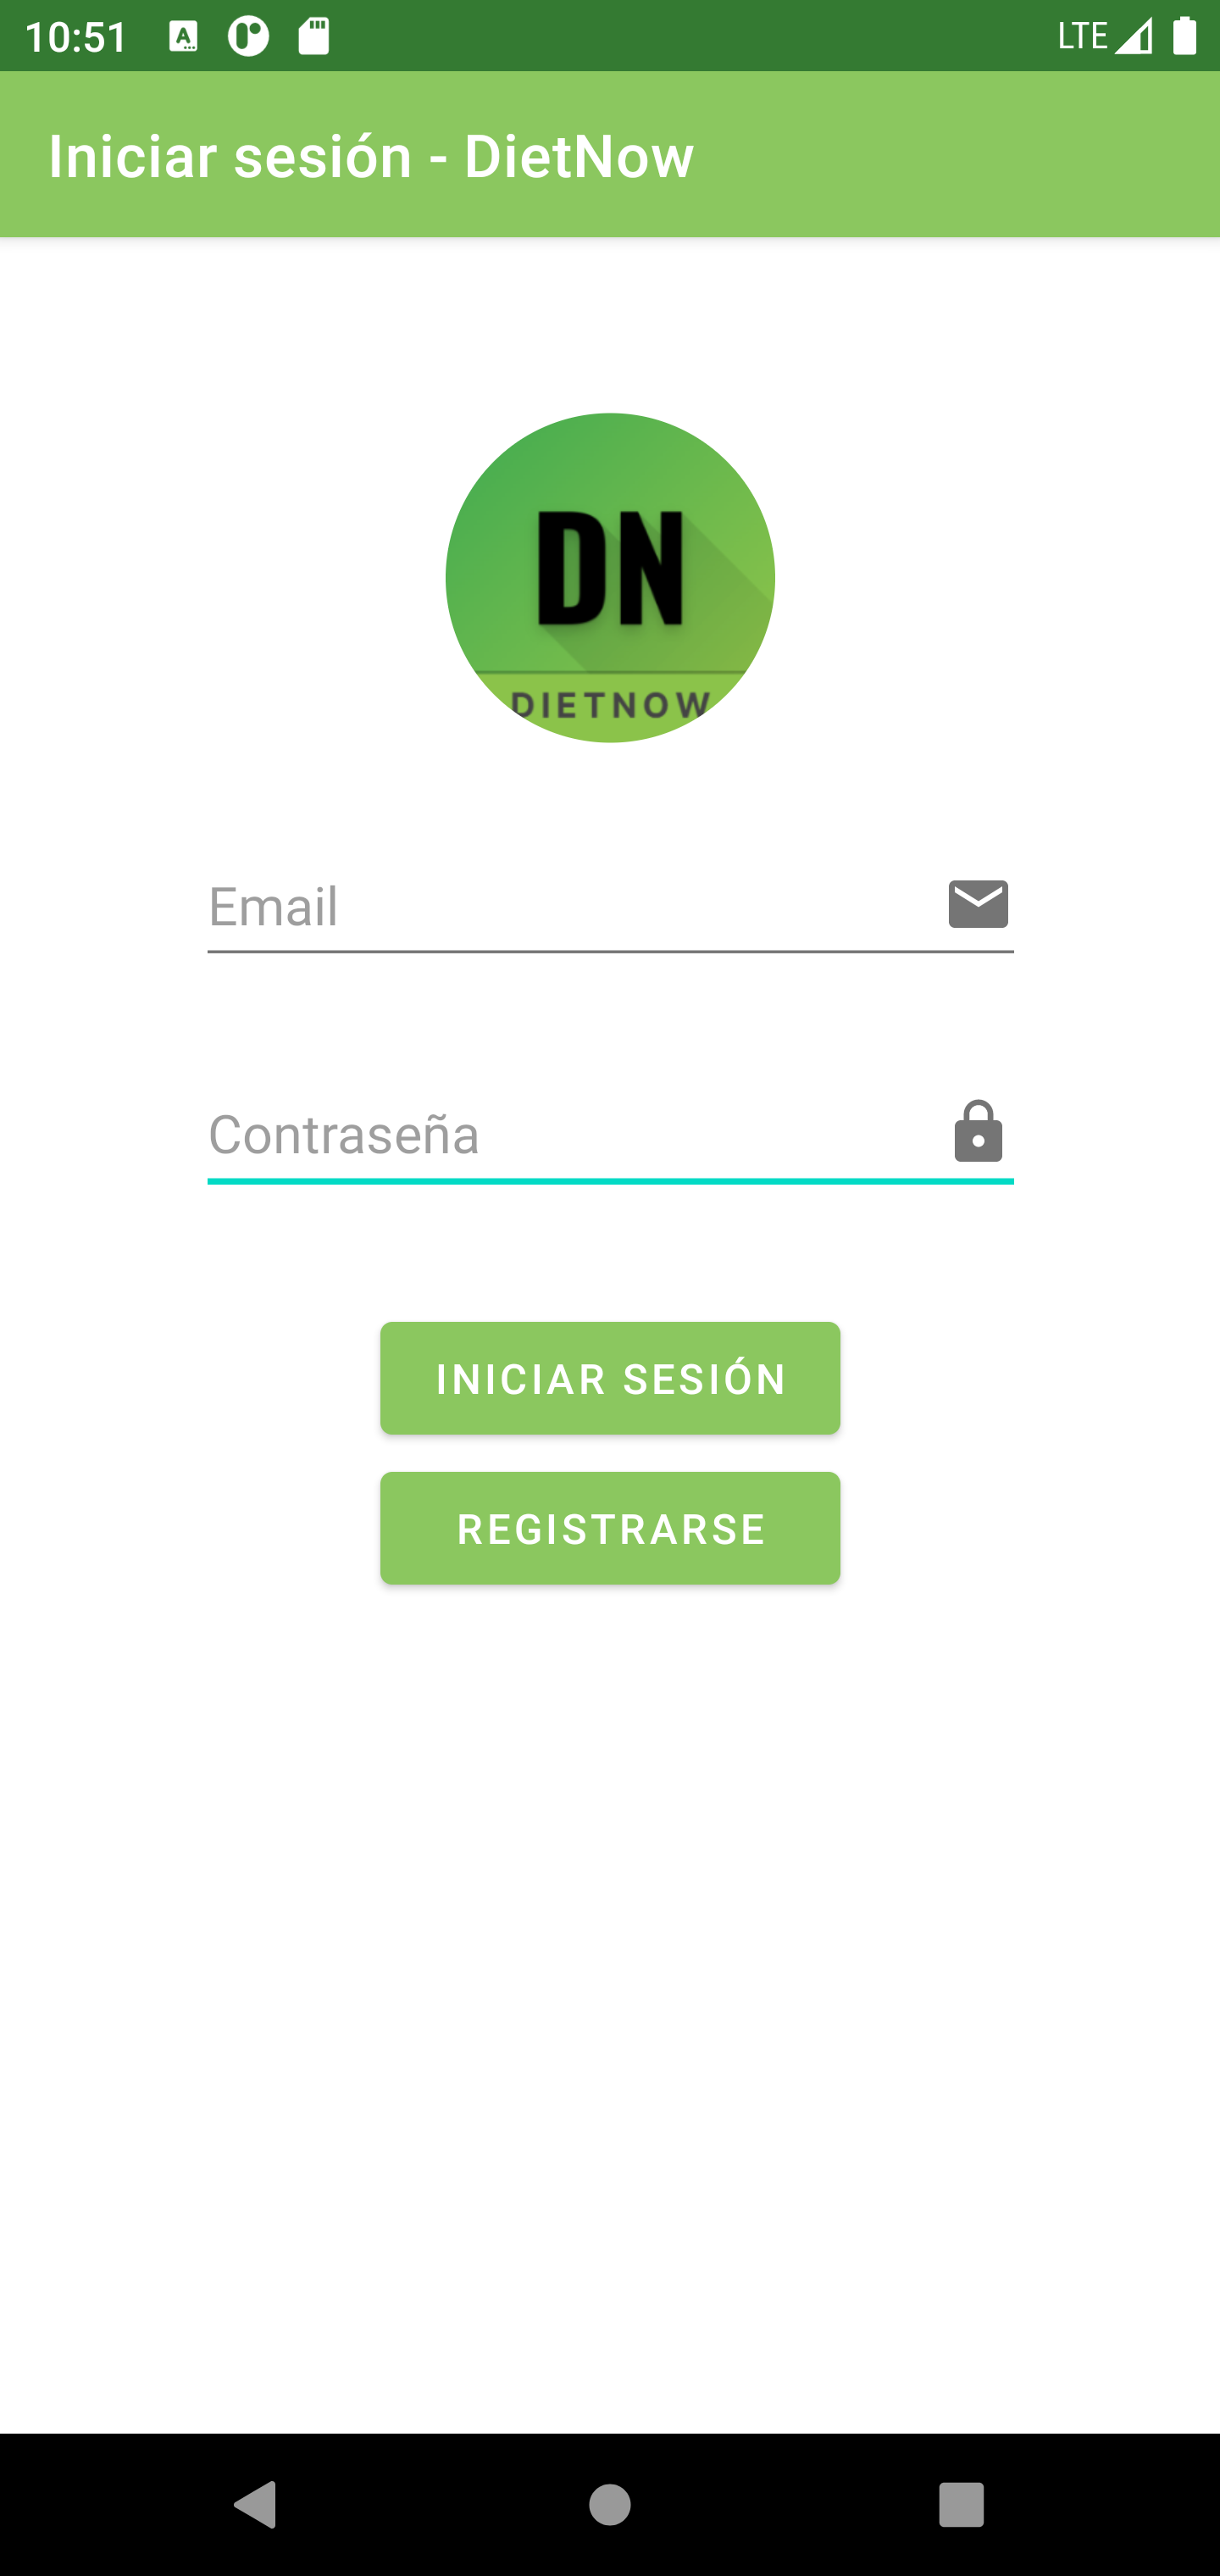
\includegraphics[width=0.4\textwidth]{Images/Annexes/Iniciar_sesion.png}}
    \subfigure[Vista de registro]{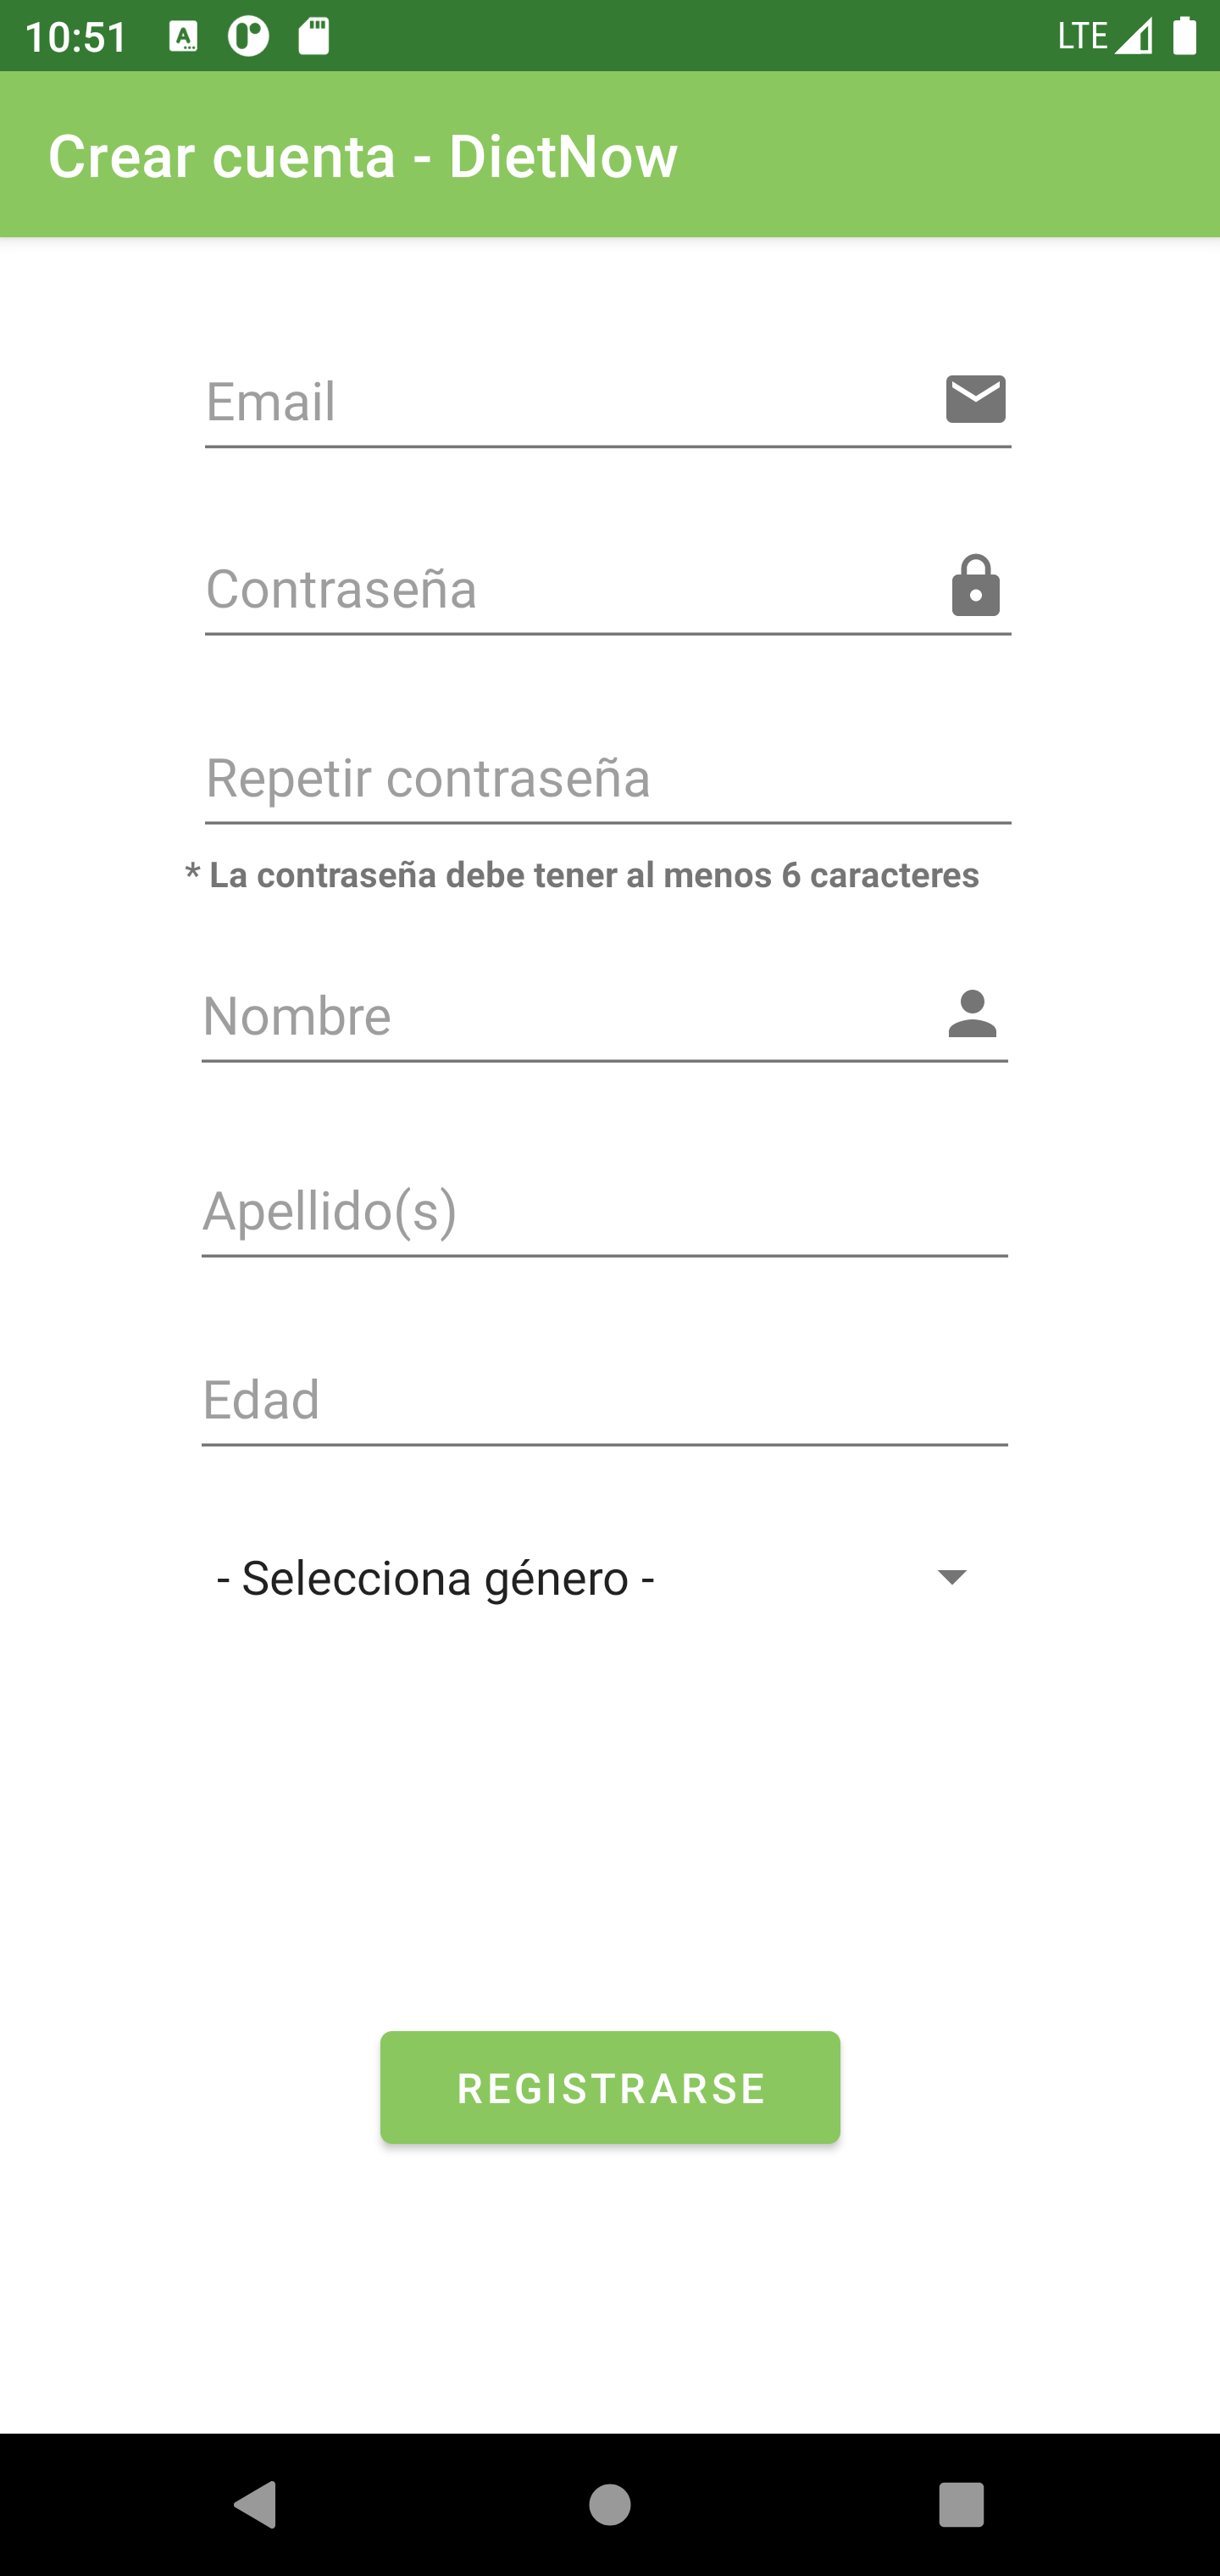
\includegraphics[width=0.4\textwidth]{Images/Annexes/Registrarse.png}}
    \caption{Vistas de la aplicación}
    \label{fig:vista_registrarse}
\end{figure}

Cuando se accede a la aplicación lo primero que aparece es el menú principal \ref{fig:vista_principal}, que en función del rol que tenga el usuario verá más o menos opciones, desde este menú se puede acceder a todas las funcionalidades de la aplicación siempre y cuando se tengan los permisos para ello. Los roles son Usuario y Administrador.

\begin{figure}[H]
    \centering
    \subfigure[Menú principal deportistas]{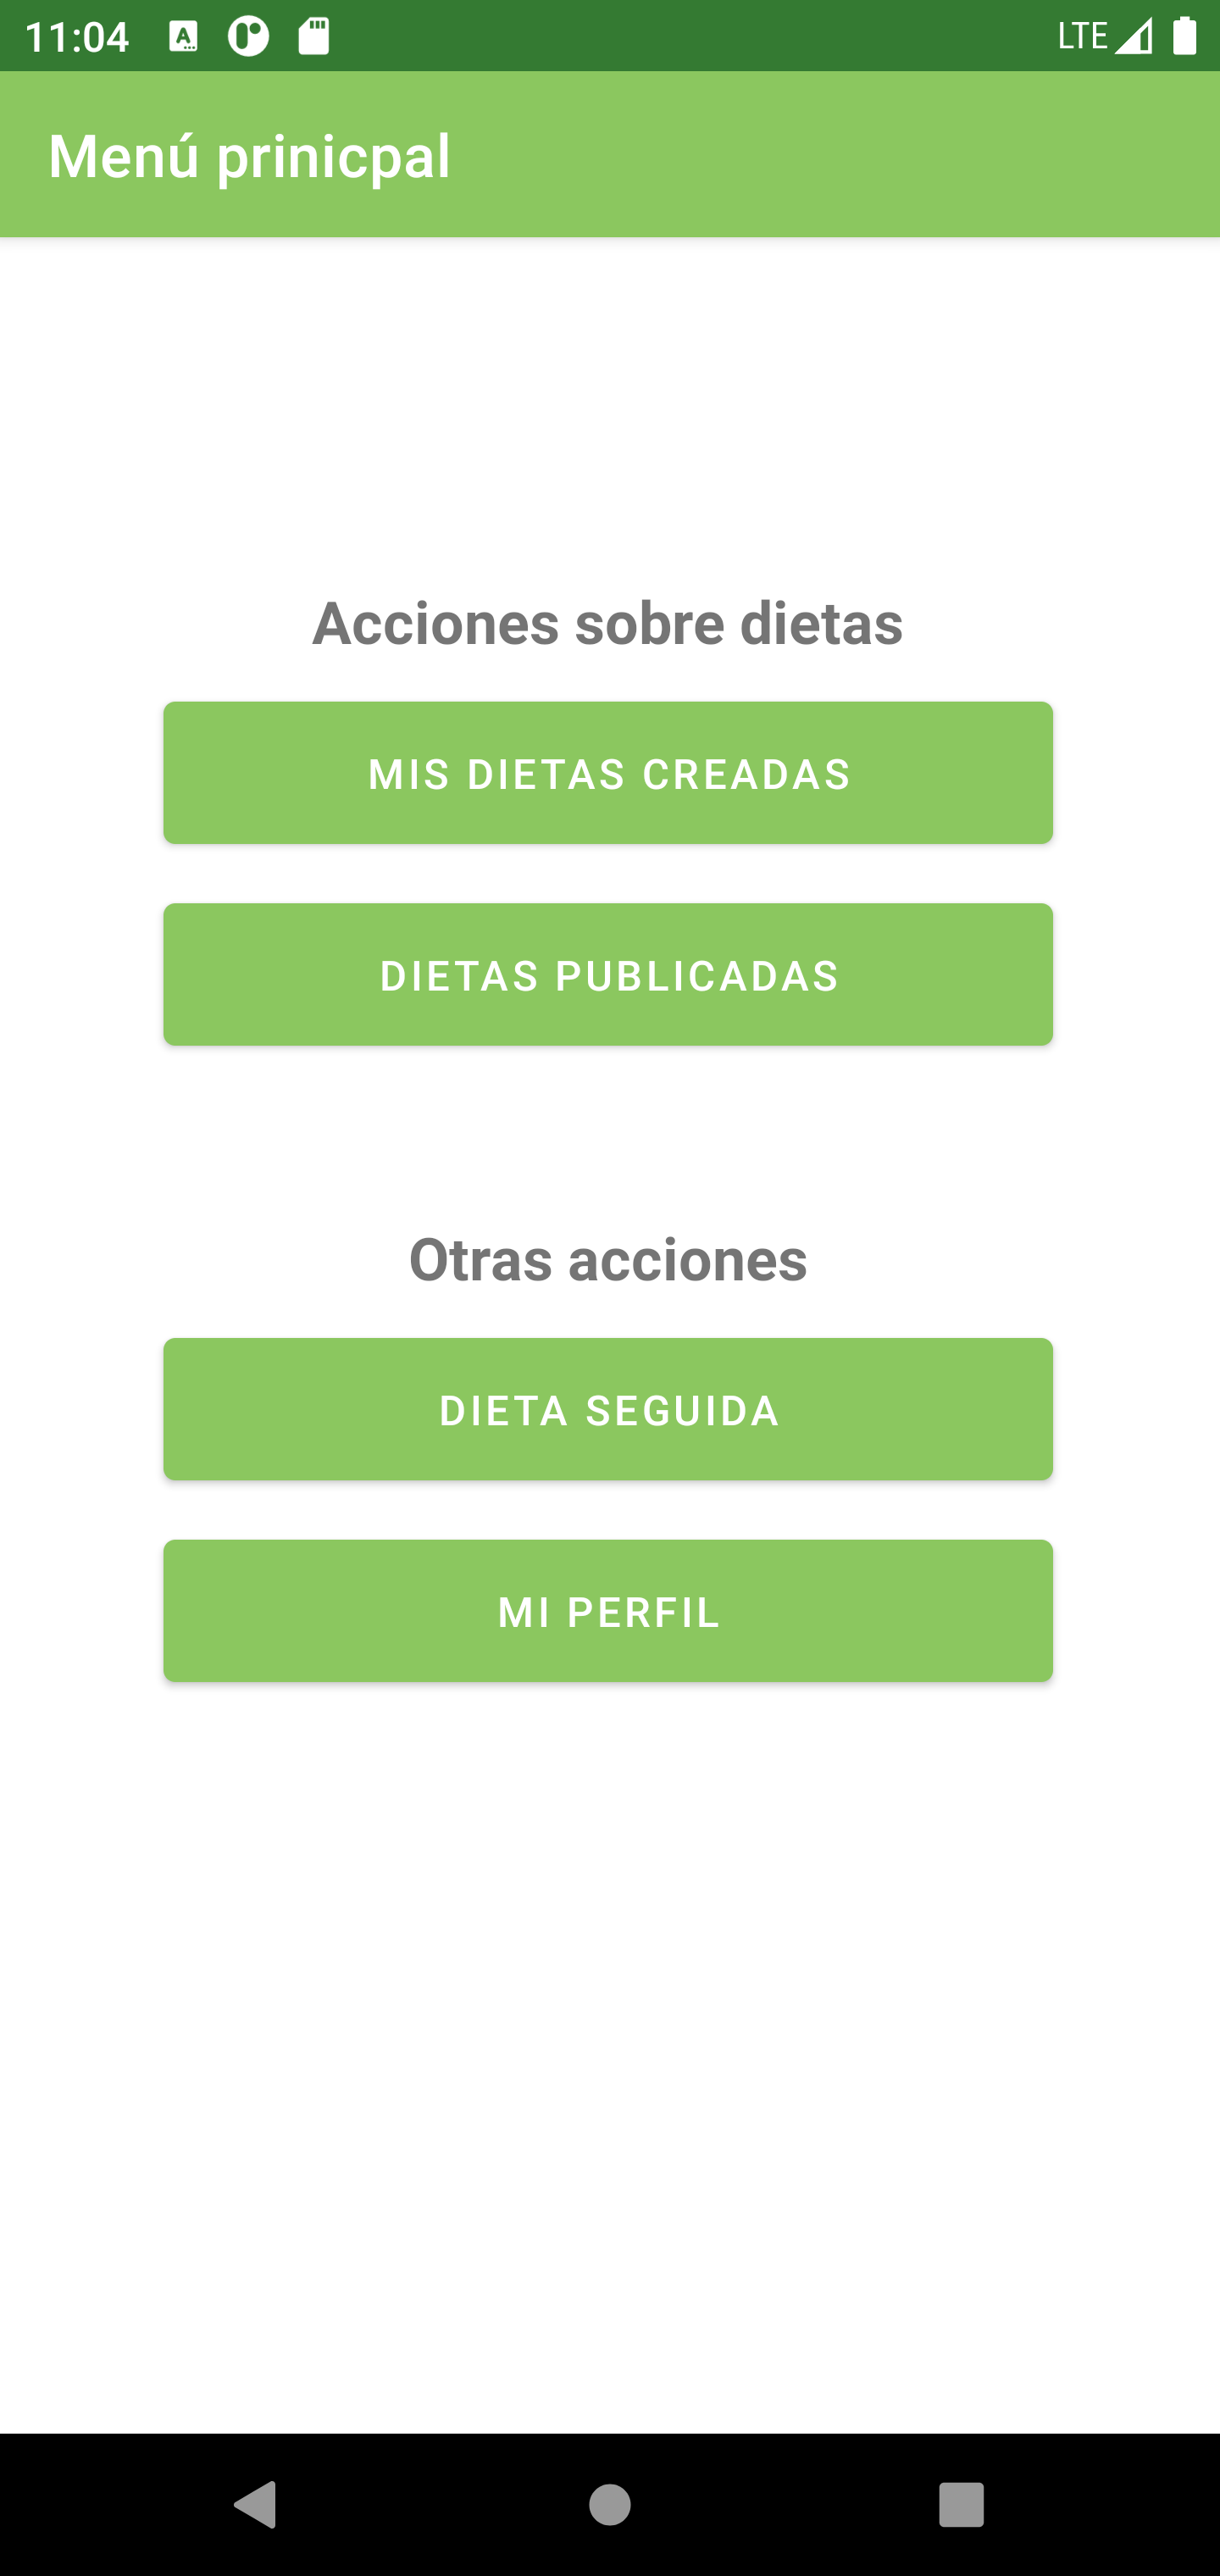
\includegraphics[width=0.4\textwidth]{Images/Annexes/Menu_usuarios.png}}
    \subfigure[Menú principal administradores]{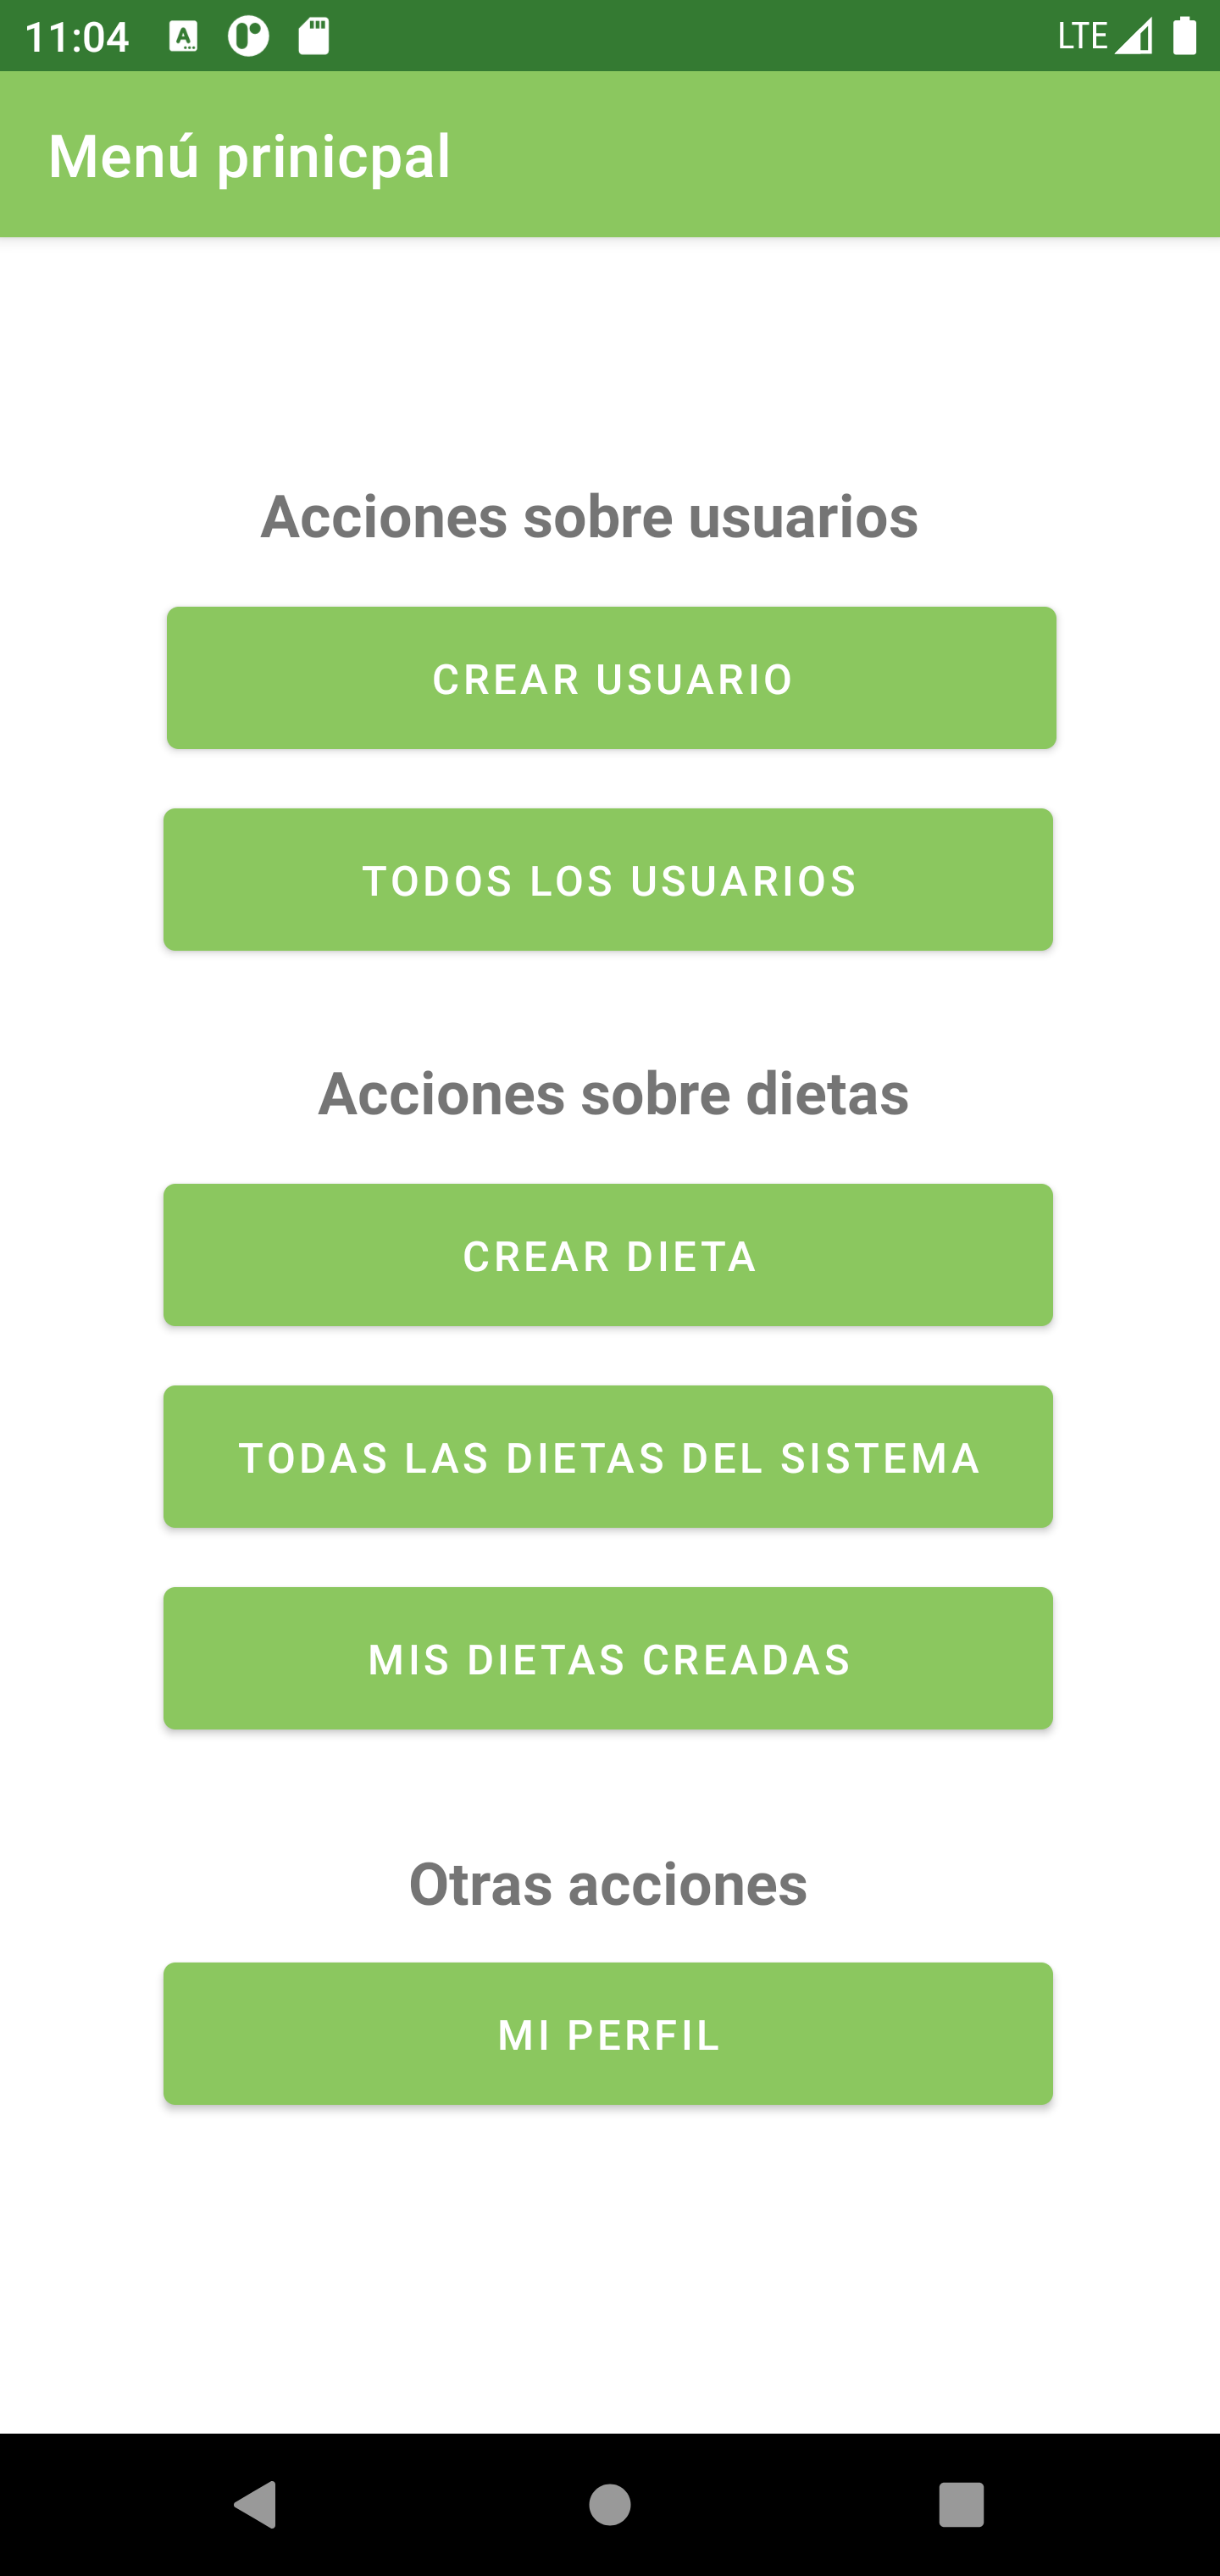
\includegraphics[width=0.4\textwidth]{Images/Annexes/Menu_administradores.png}}
    \caption{Menú principal de la aplicación}
    \label{fig:vista_principal}
\end{figure}


\section{Usuarios}
El grueso de la aplicación tiene este rol, los módulos a los que pueden acceder son todos los de dieta y perfil.
\subsection{Mis dietas creadas} \label{user_my_created_diets}
Si el usuario pulsa mis dietas creadas verá un listado de dietas que ha creado, como se muestra en la figura \ref{fig:mis_dietas}, si no ha creado ninguna o es un nuevo usuario no verá ninguna dieta. En caso de tener dietas el usuario podrá ver el detalle de cada una pulsando en el botón ``Ver dieta``, crear una dieta nueva pulsando el botón con símbolo ``$+$`` ubicado en la esquina inferior derecha o filtrar las dietas con un buscador dinámico que se activa al pulsar la lupa que se encuentra arriba del todo.

\begin{figure}[H]
    \centering
    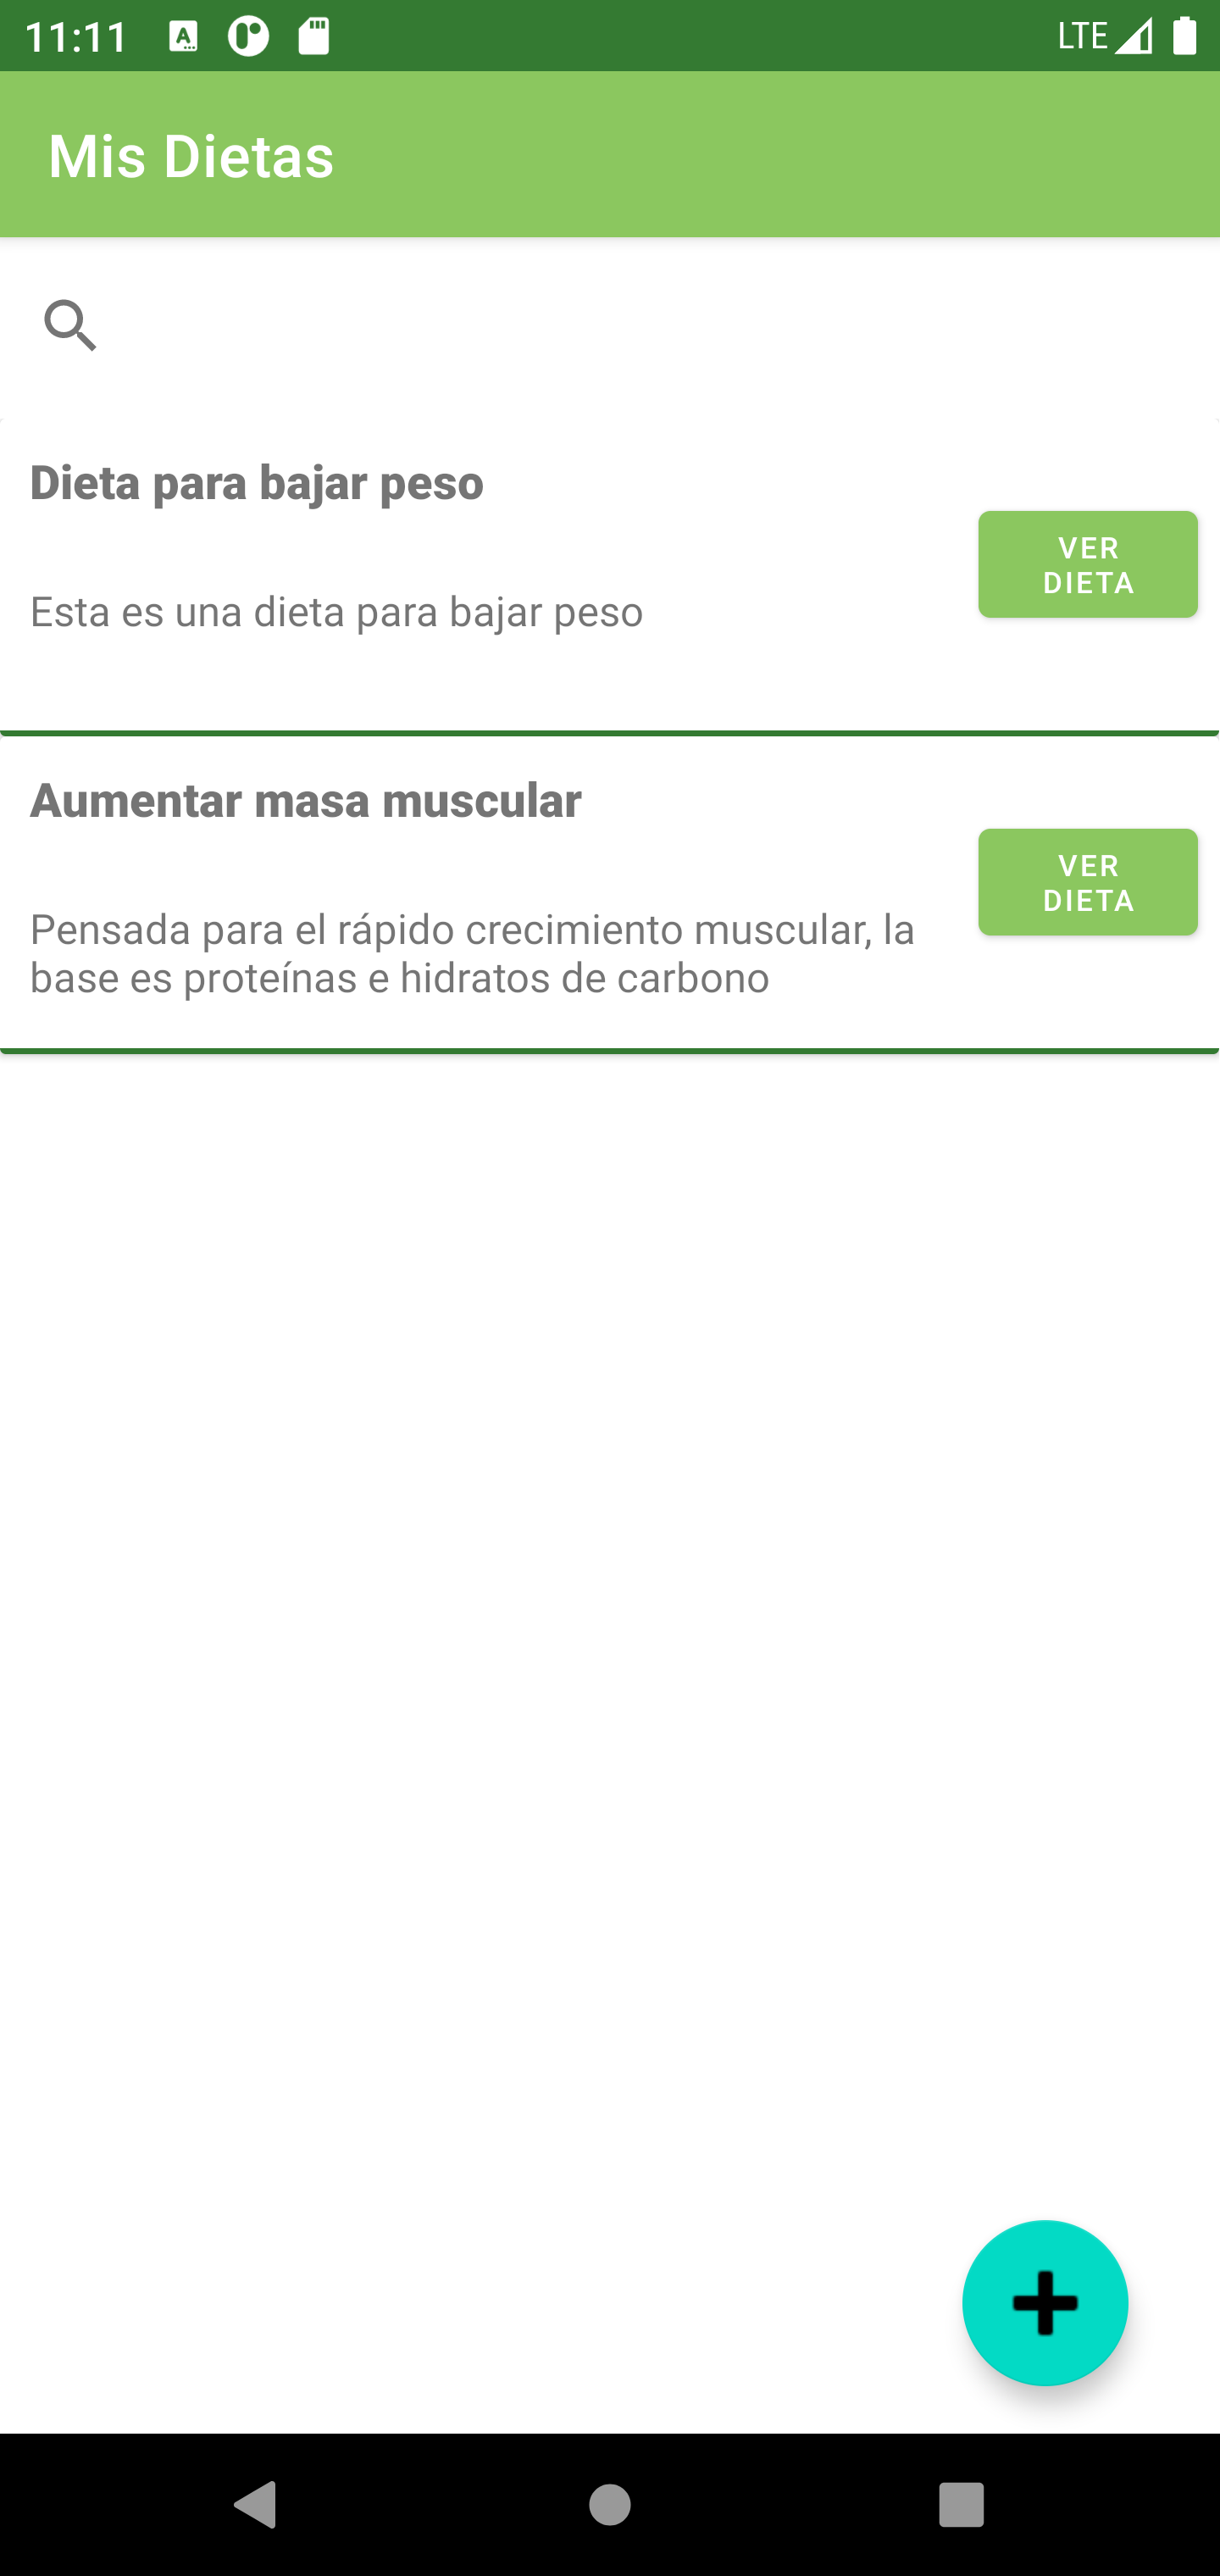
\includegraphics[width=0.5\textwidth]{Images/Annexes/mis_dietas.png}
    \caption{Vista detallada de un documento de una dieta}
    \label{fig:mis_dietas}
\end{figure}

Al presionar “ver dieta” el usuario accede la información detallada de la dieta \ref{fig:mis_dietas_info} y al ser su autor puede editar o eliminar la dieta,  publicarla para el resto de los usuarios o despublicarla si ya estaba publicada. Si la dieta está publicada aparecerá la opción de acceder a los comentarios de la dieta.
\begin{figure}[H]
    \centering
    \subfigure{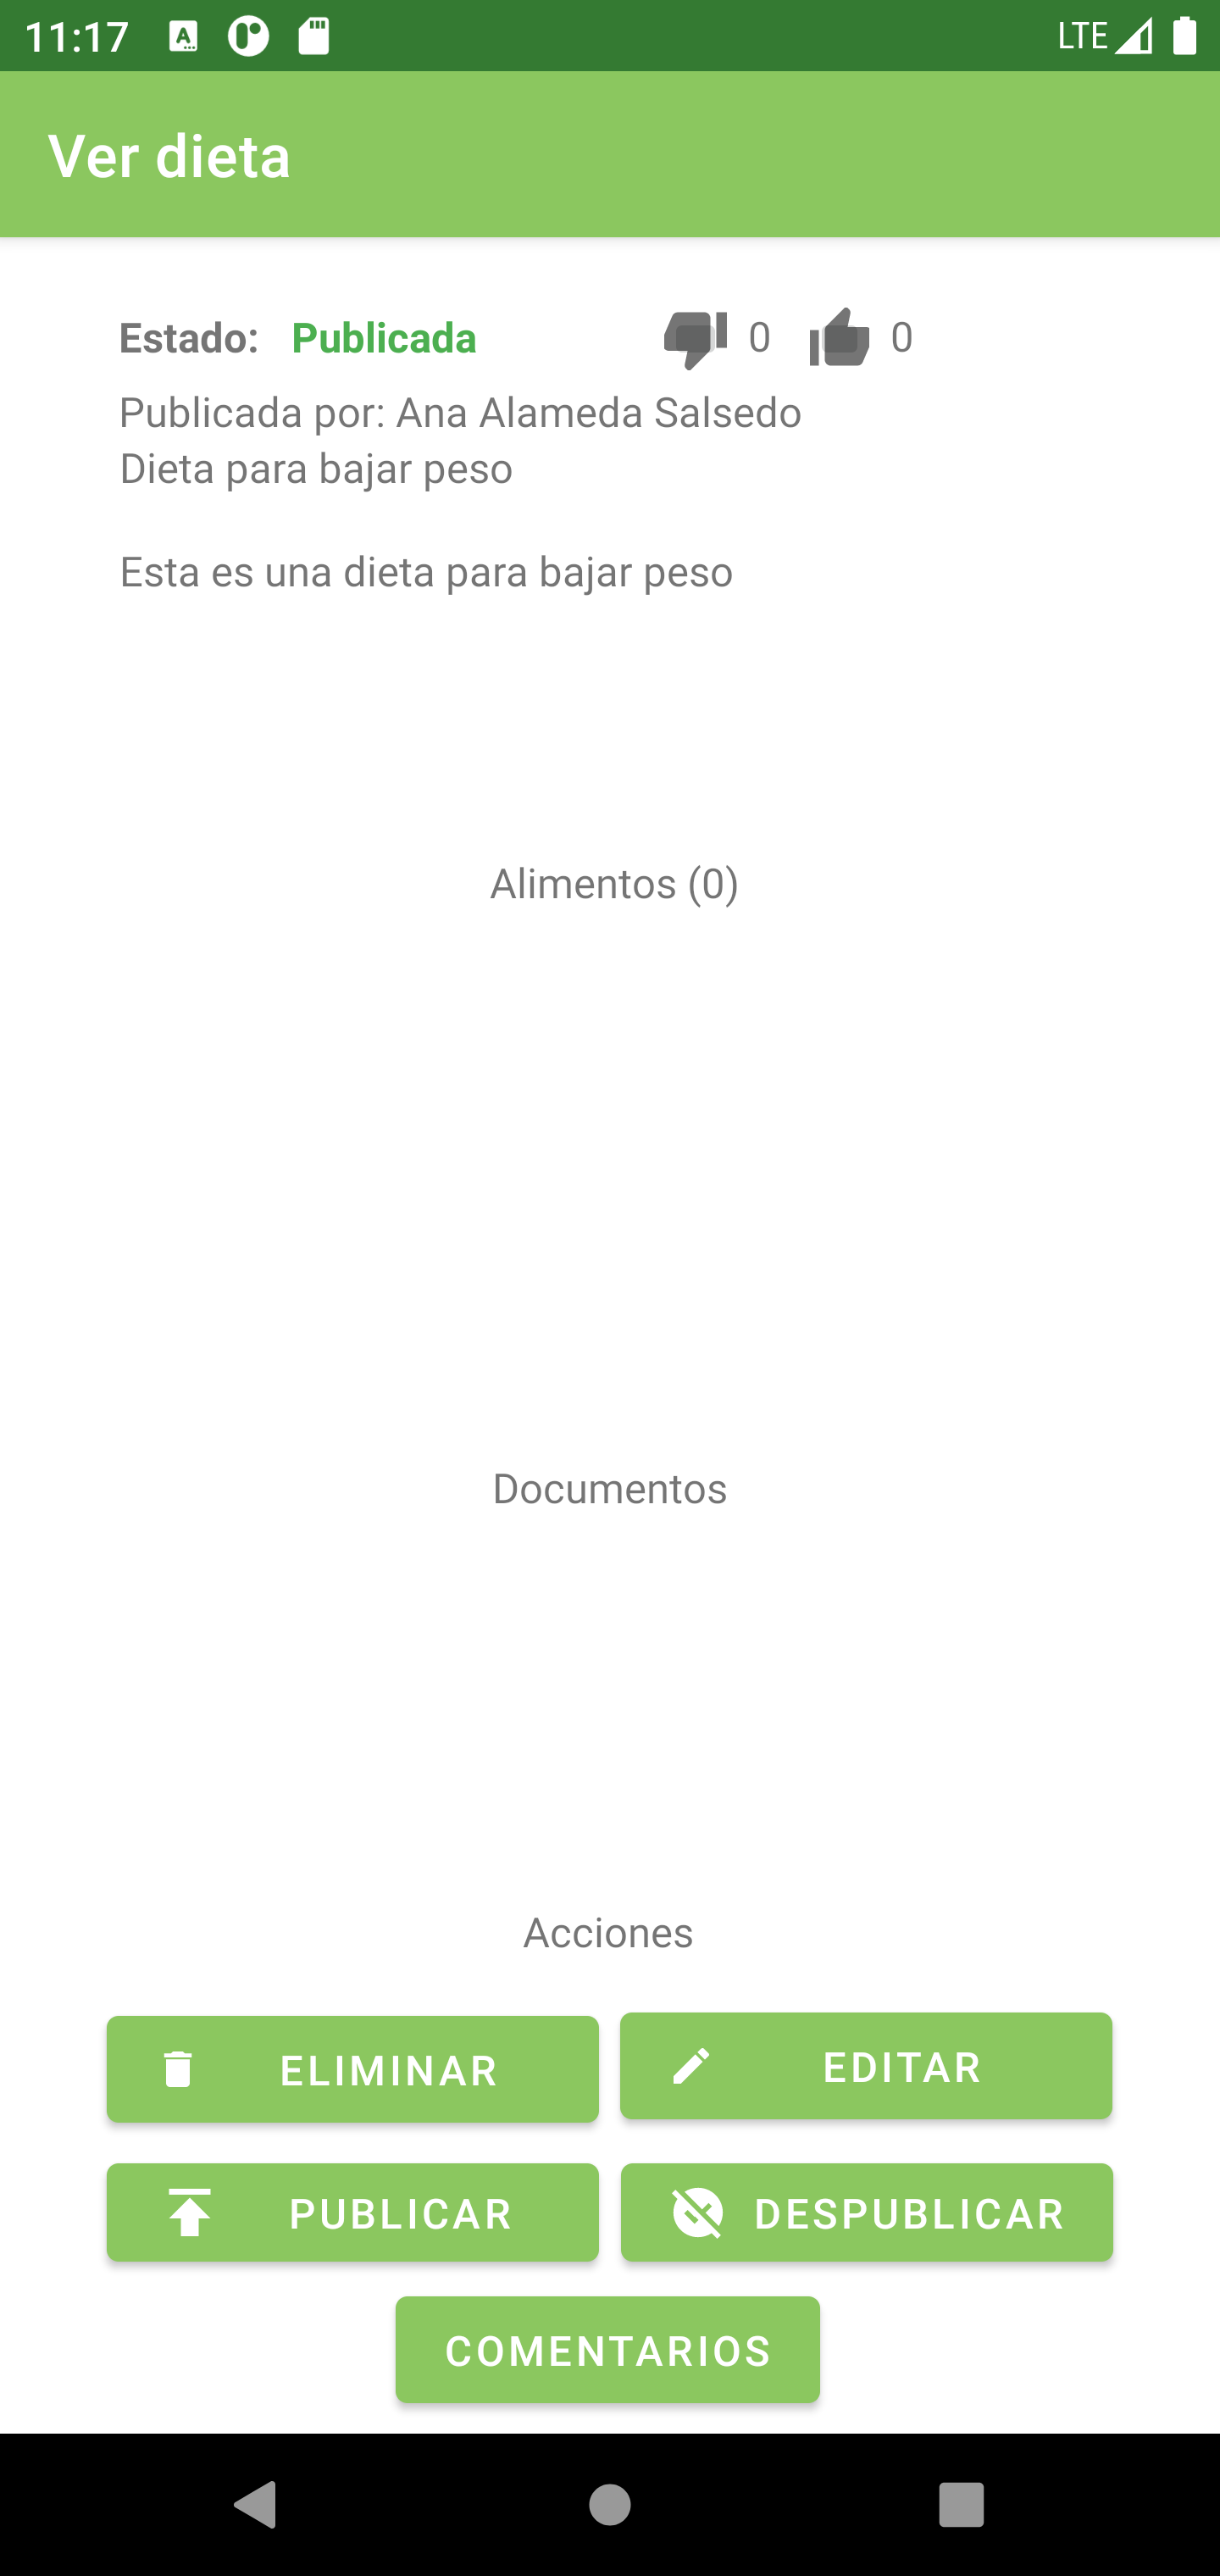
\includegraphics[width=0.4\textwidth]{Images/Annexes/ver_dieta_publicada.png}}
    \subfigure{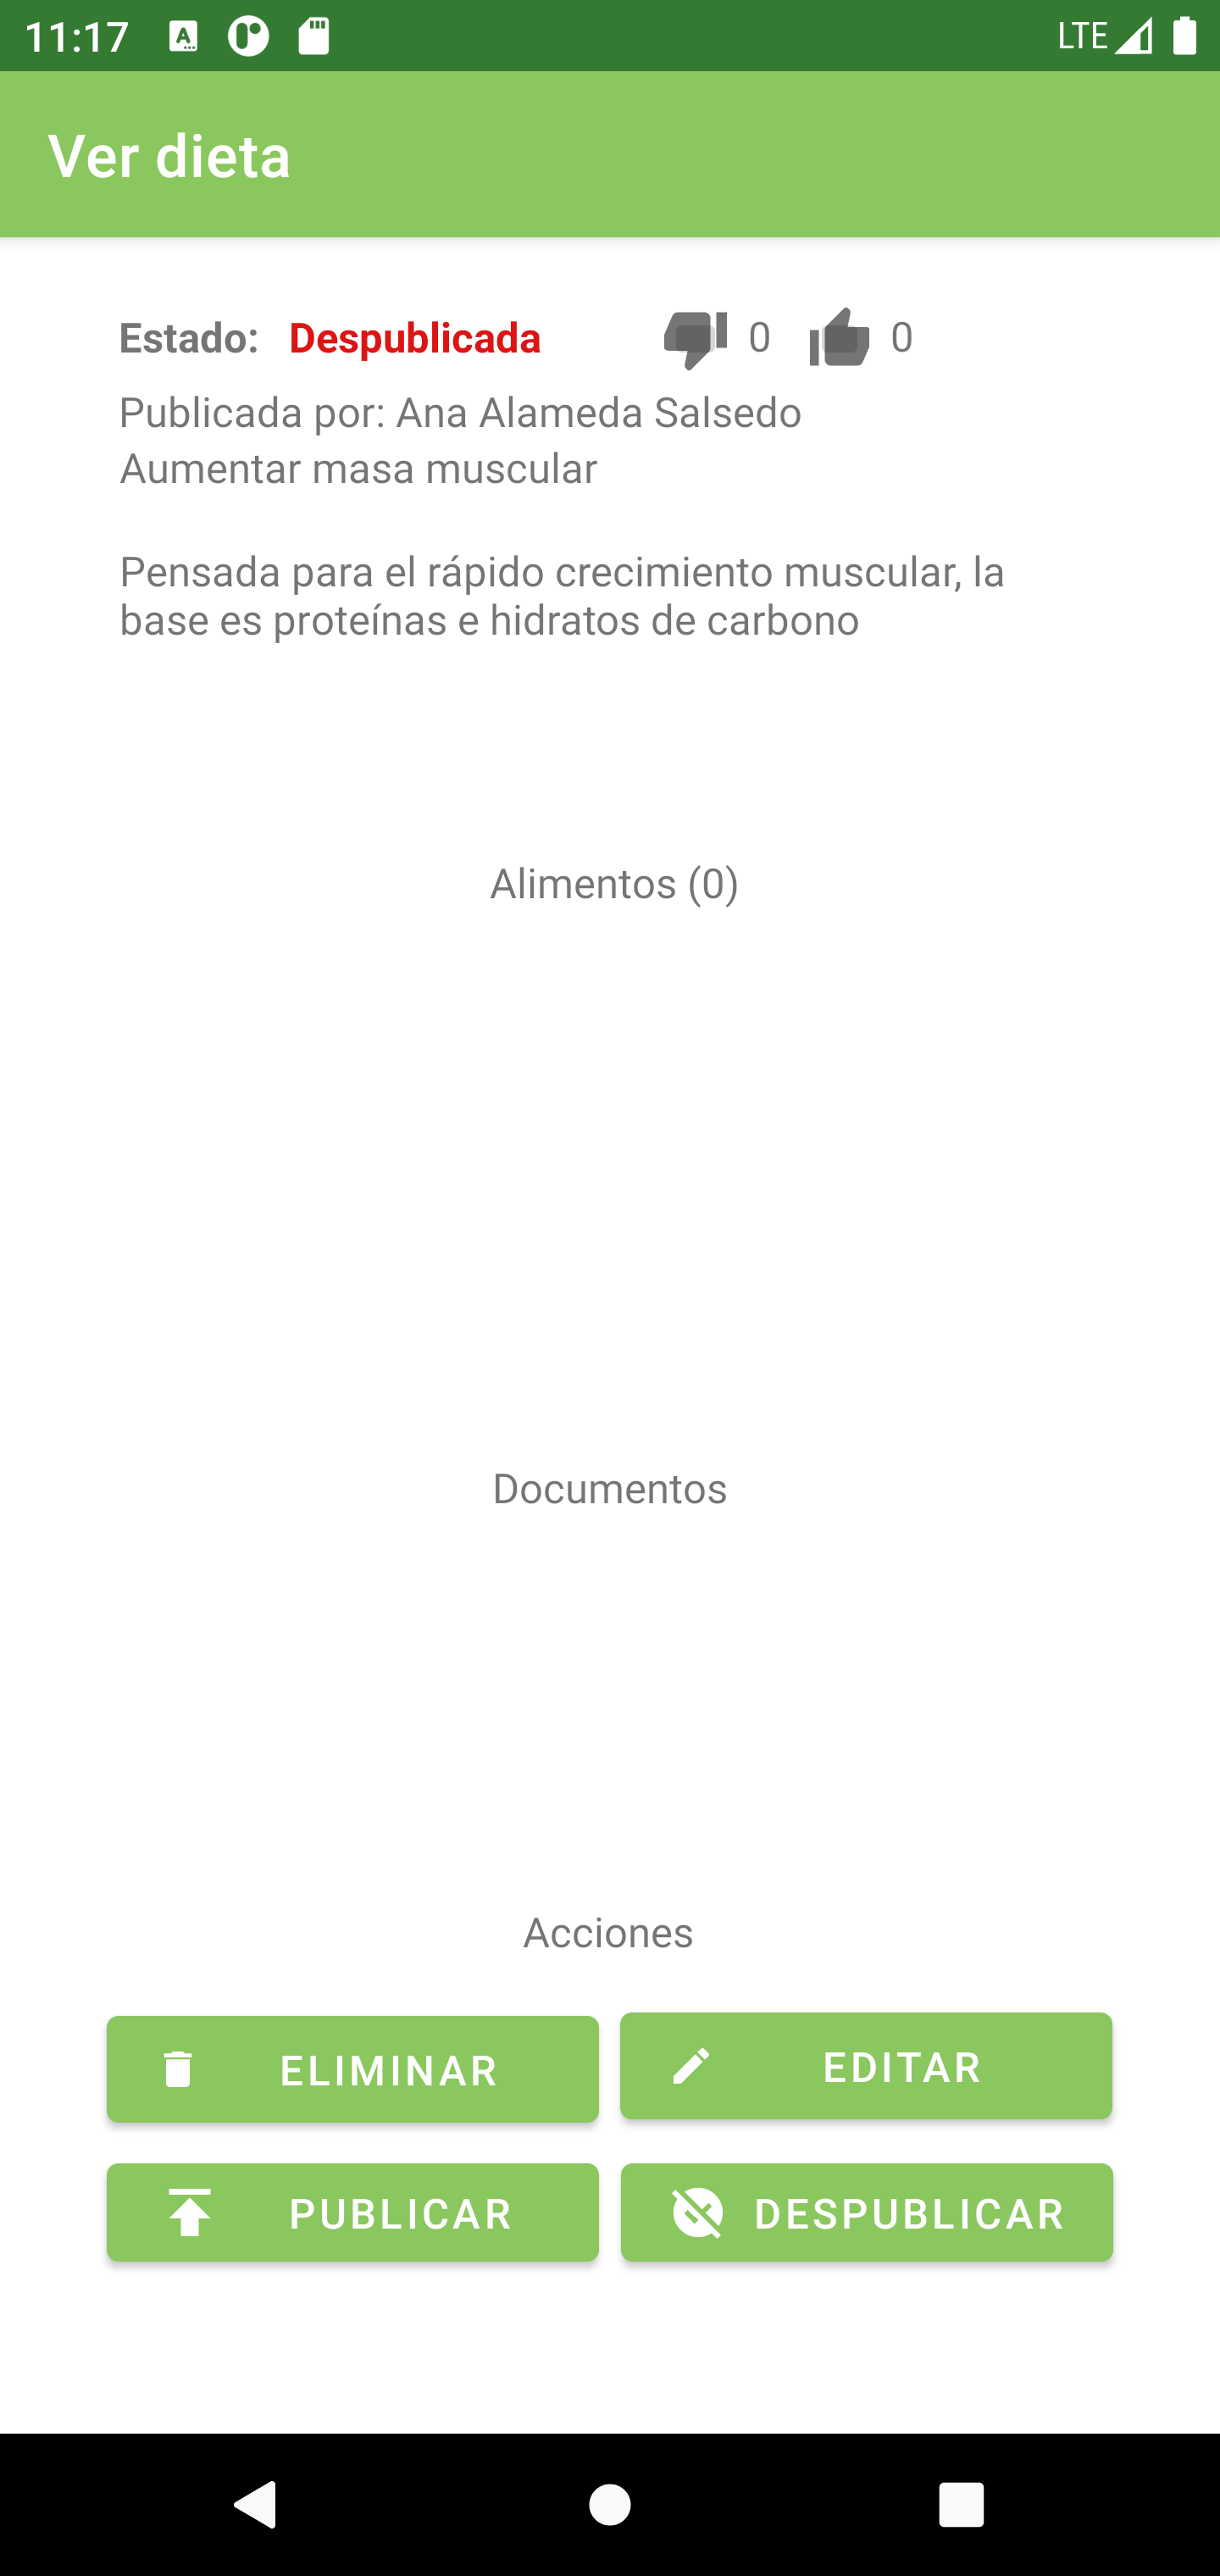
\includegraphics[width=0.4\textwidth]{Images/Annexes/ver_dieta_despublicada.png}}
    \caption{Una dieta publicada y despublicada}
    \label{fig:mis_dietas_info}
\end{figure}

Si el usuario presiona editar podrá añadir alimentos a la dieta y/o subir documentos en formato PDF con información que el usuario considere necesaria para la dieta como por ejemplo aportar estudios que la respalden.

Para añadir un alimento el usuario dispone de varias formas, como se muestra en la figura \ref{fig:añadir_alimentos} , desde la cámara, en cuyo caso deberá escanear el código de barras del alimento o manualmente ya sea escribiendo el código de barras o escribiendo los datos del alimento campo por campo.
\begin{figure}[H]
    \centering
    \subfigure[Añadir manualmente]{\includegraphics[width=0.4\textwidth]{Images/Annexes/añadir_alimentos.png}}
    \subfigure[Añadir con cámara]{\includegraphics[width=0.4\textwidth]{Images/Annexes/añadir_alimentos_camara.jpg}}
    \caption{Vista de añadir alimentos a una dieta}
    \label{fig:añadir_alimentos}
\end{figure}


\subsection{Dietas publicadas}
Cuando el usuario accede a las dietas publicadas \ref{fig:dietas_publicadas} podrá visualizar todas las dietas que los usuarios de DietNow han creado y publicado para que estén al alcance de todos, el usuario dispondrá de un buscador dinámico en la parte de arriba para poder filtrar rápidamente las dietas por palabras clave. 

Para cada dieta publicada podrá visualizar el número de ``Me gusta`` que tiene y el número de visualizaciones y al presionar el botón ``ver dieta`` podrá visualizar el contenido de la dieta además de empezar a seguirla presionando el botón con forma de estrella o abrir la sección de comentarios para leer los comentarios y/o dejar el suyo propio.
\begin{figure}[H]
    \centering
    \subfigure[Todas las dietas publicadas]{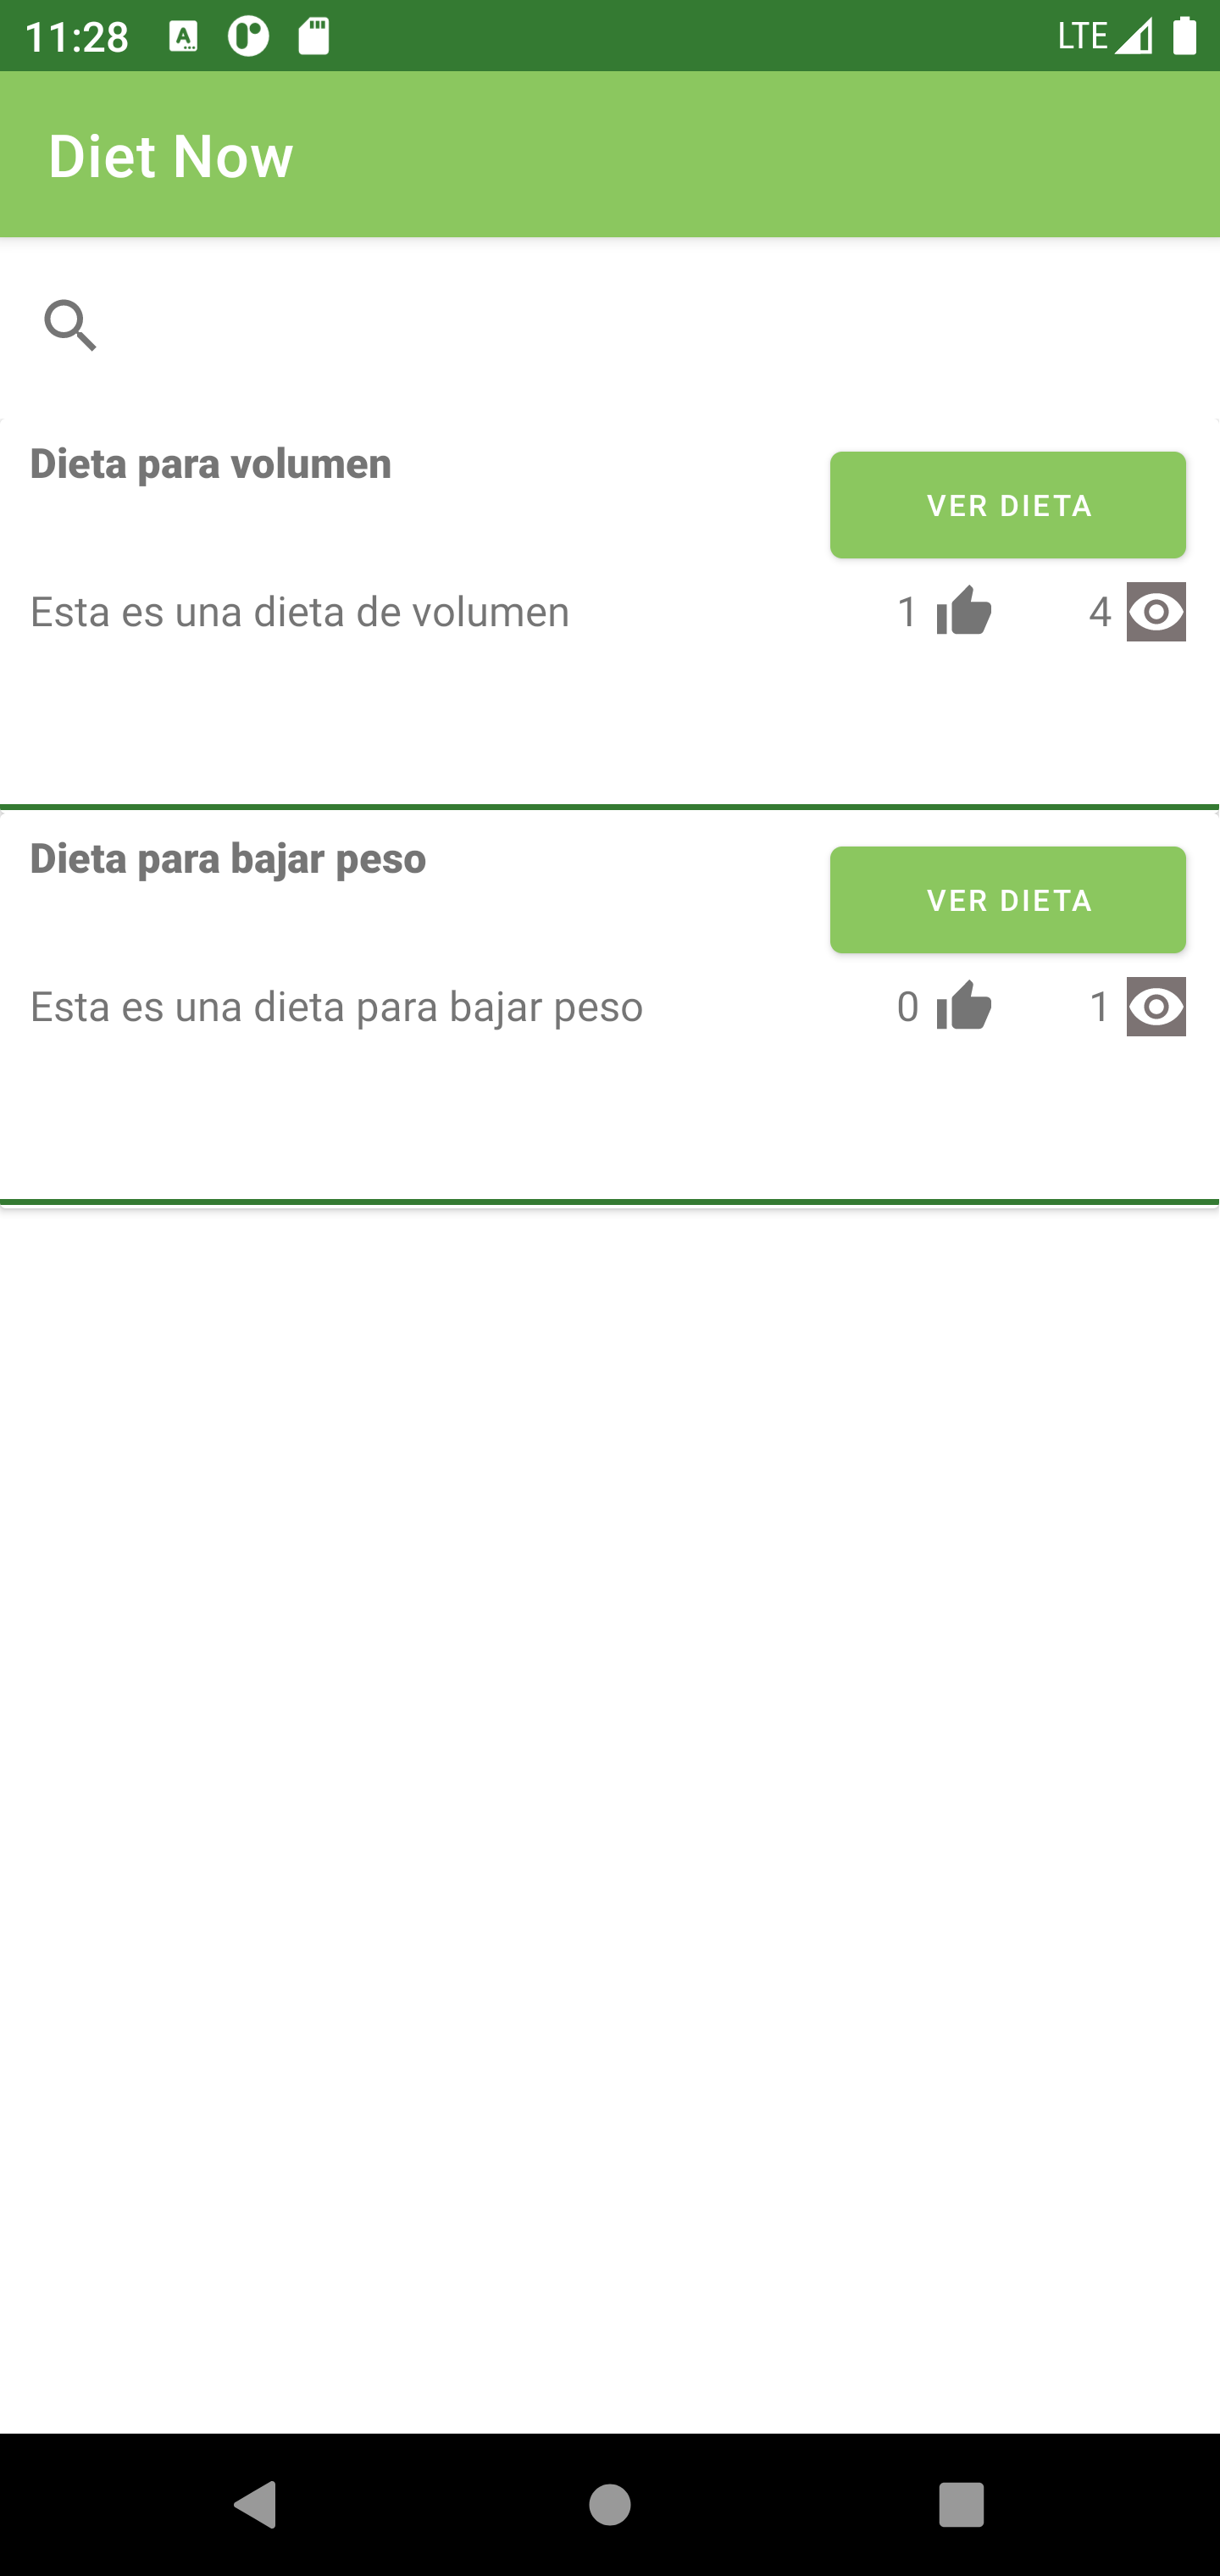
\includegraphics[width=0.4\textwidth]{Images/Annexes/vista_dietas_publicadas.png}}
    \subfigure[Vista detallada de dieta]{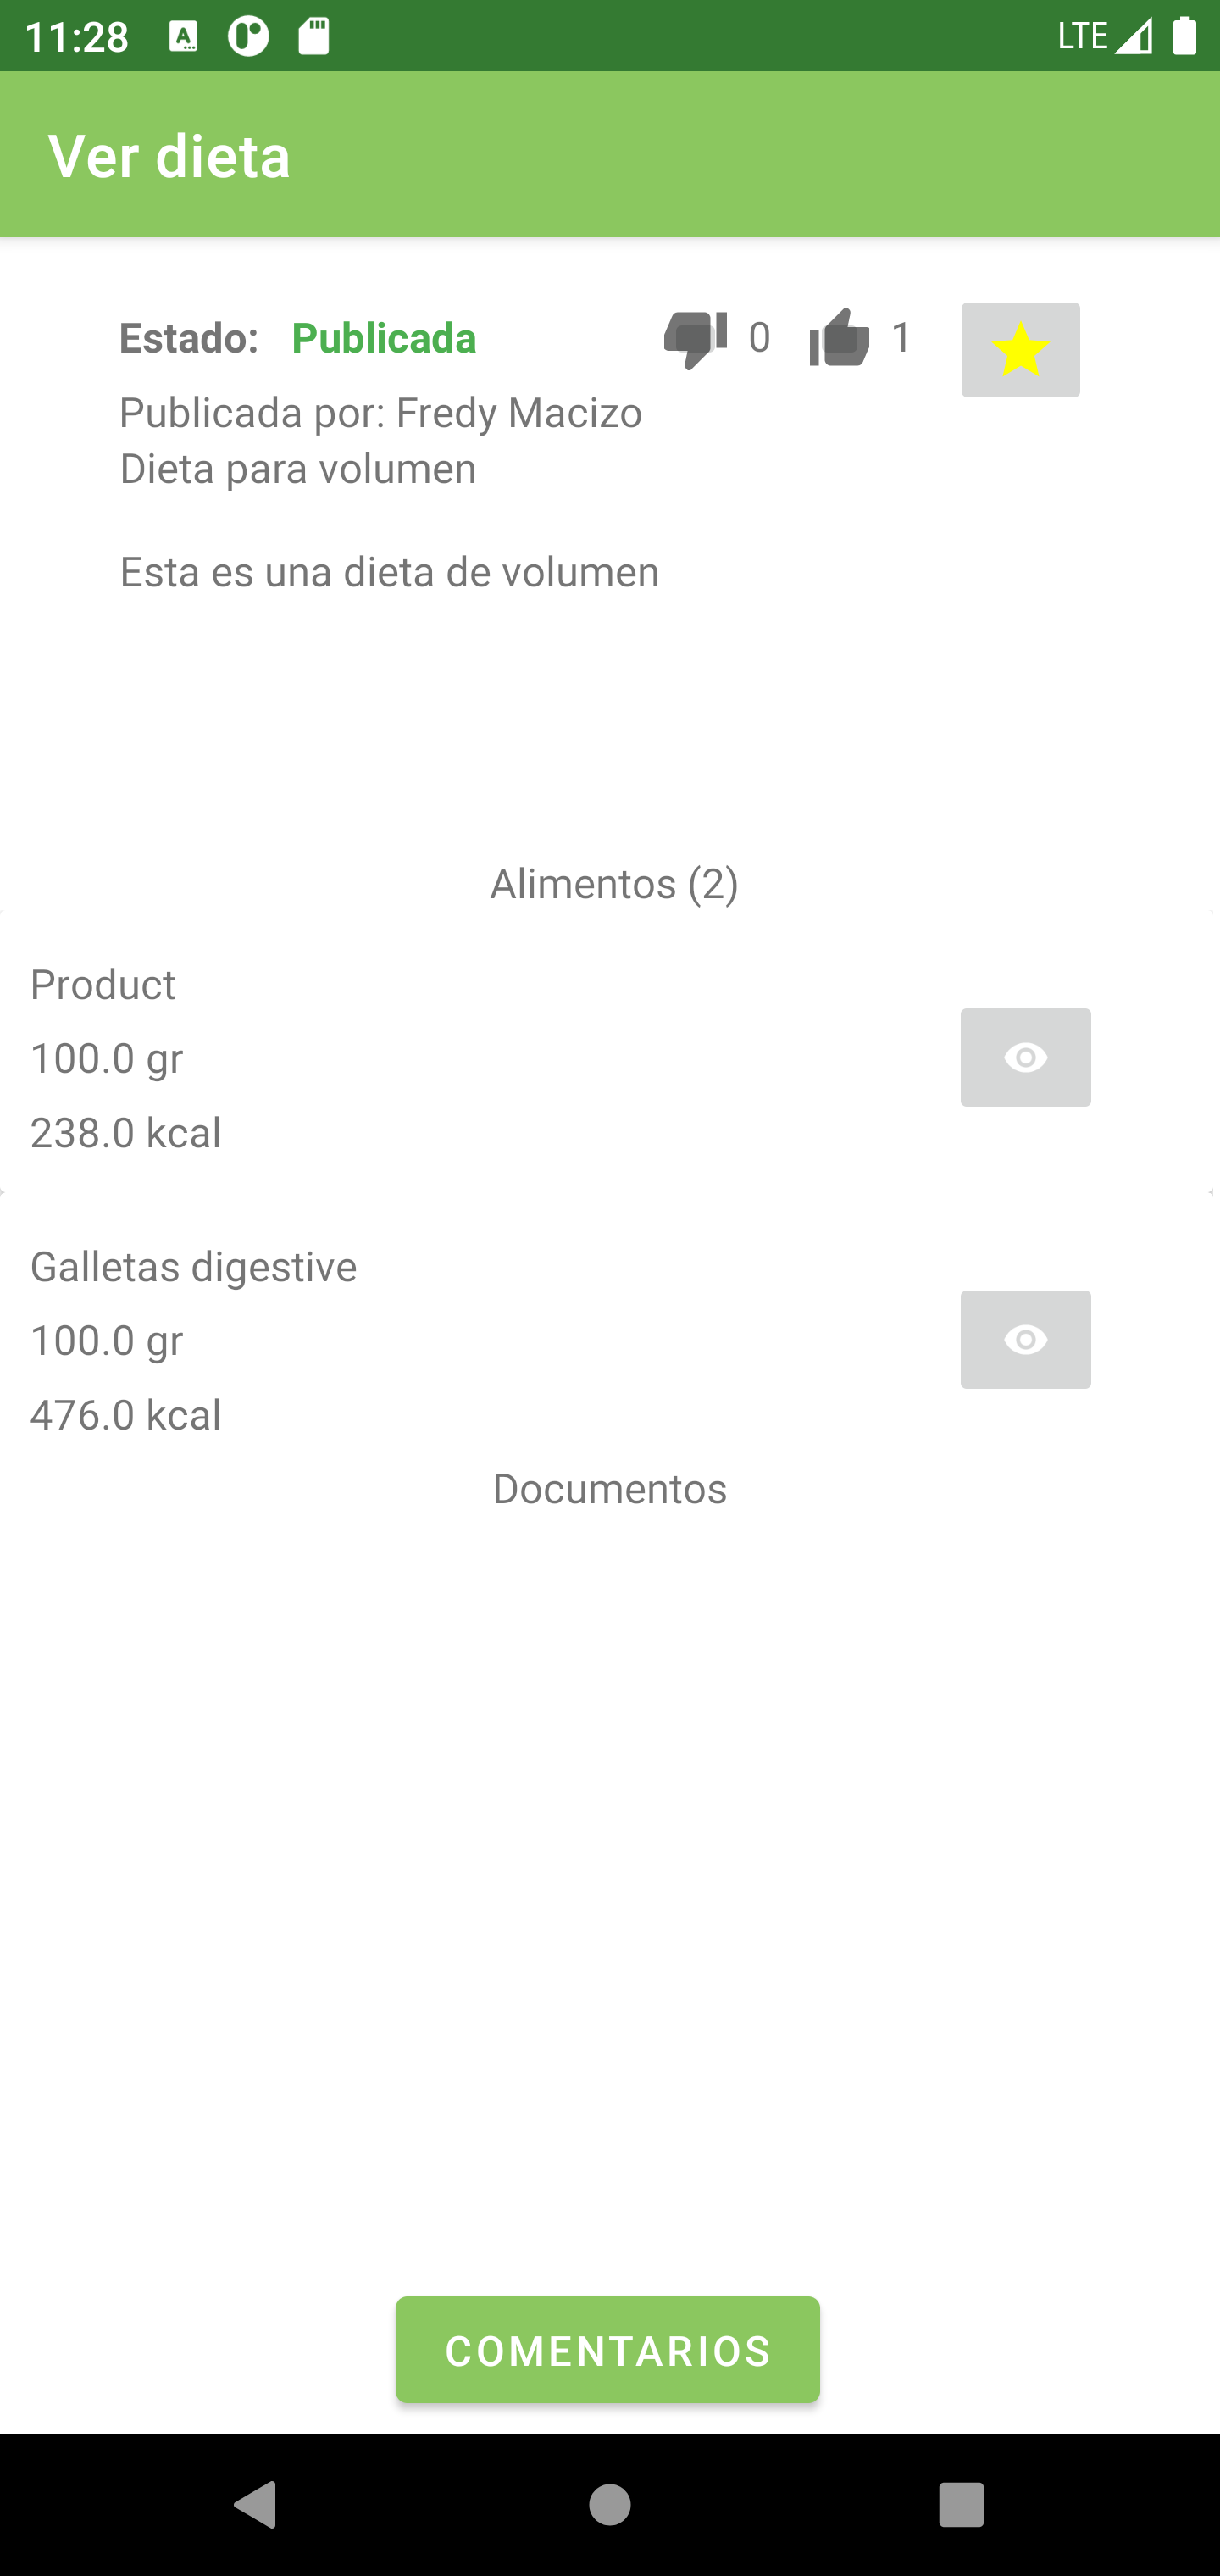
\includegraphics[width=0.4\textwidth]{Images/Annexes/vista_dieta_publicada_seguida.png}}
    % \subfigure[Vista de los comentarios de la dietas seguida]{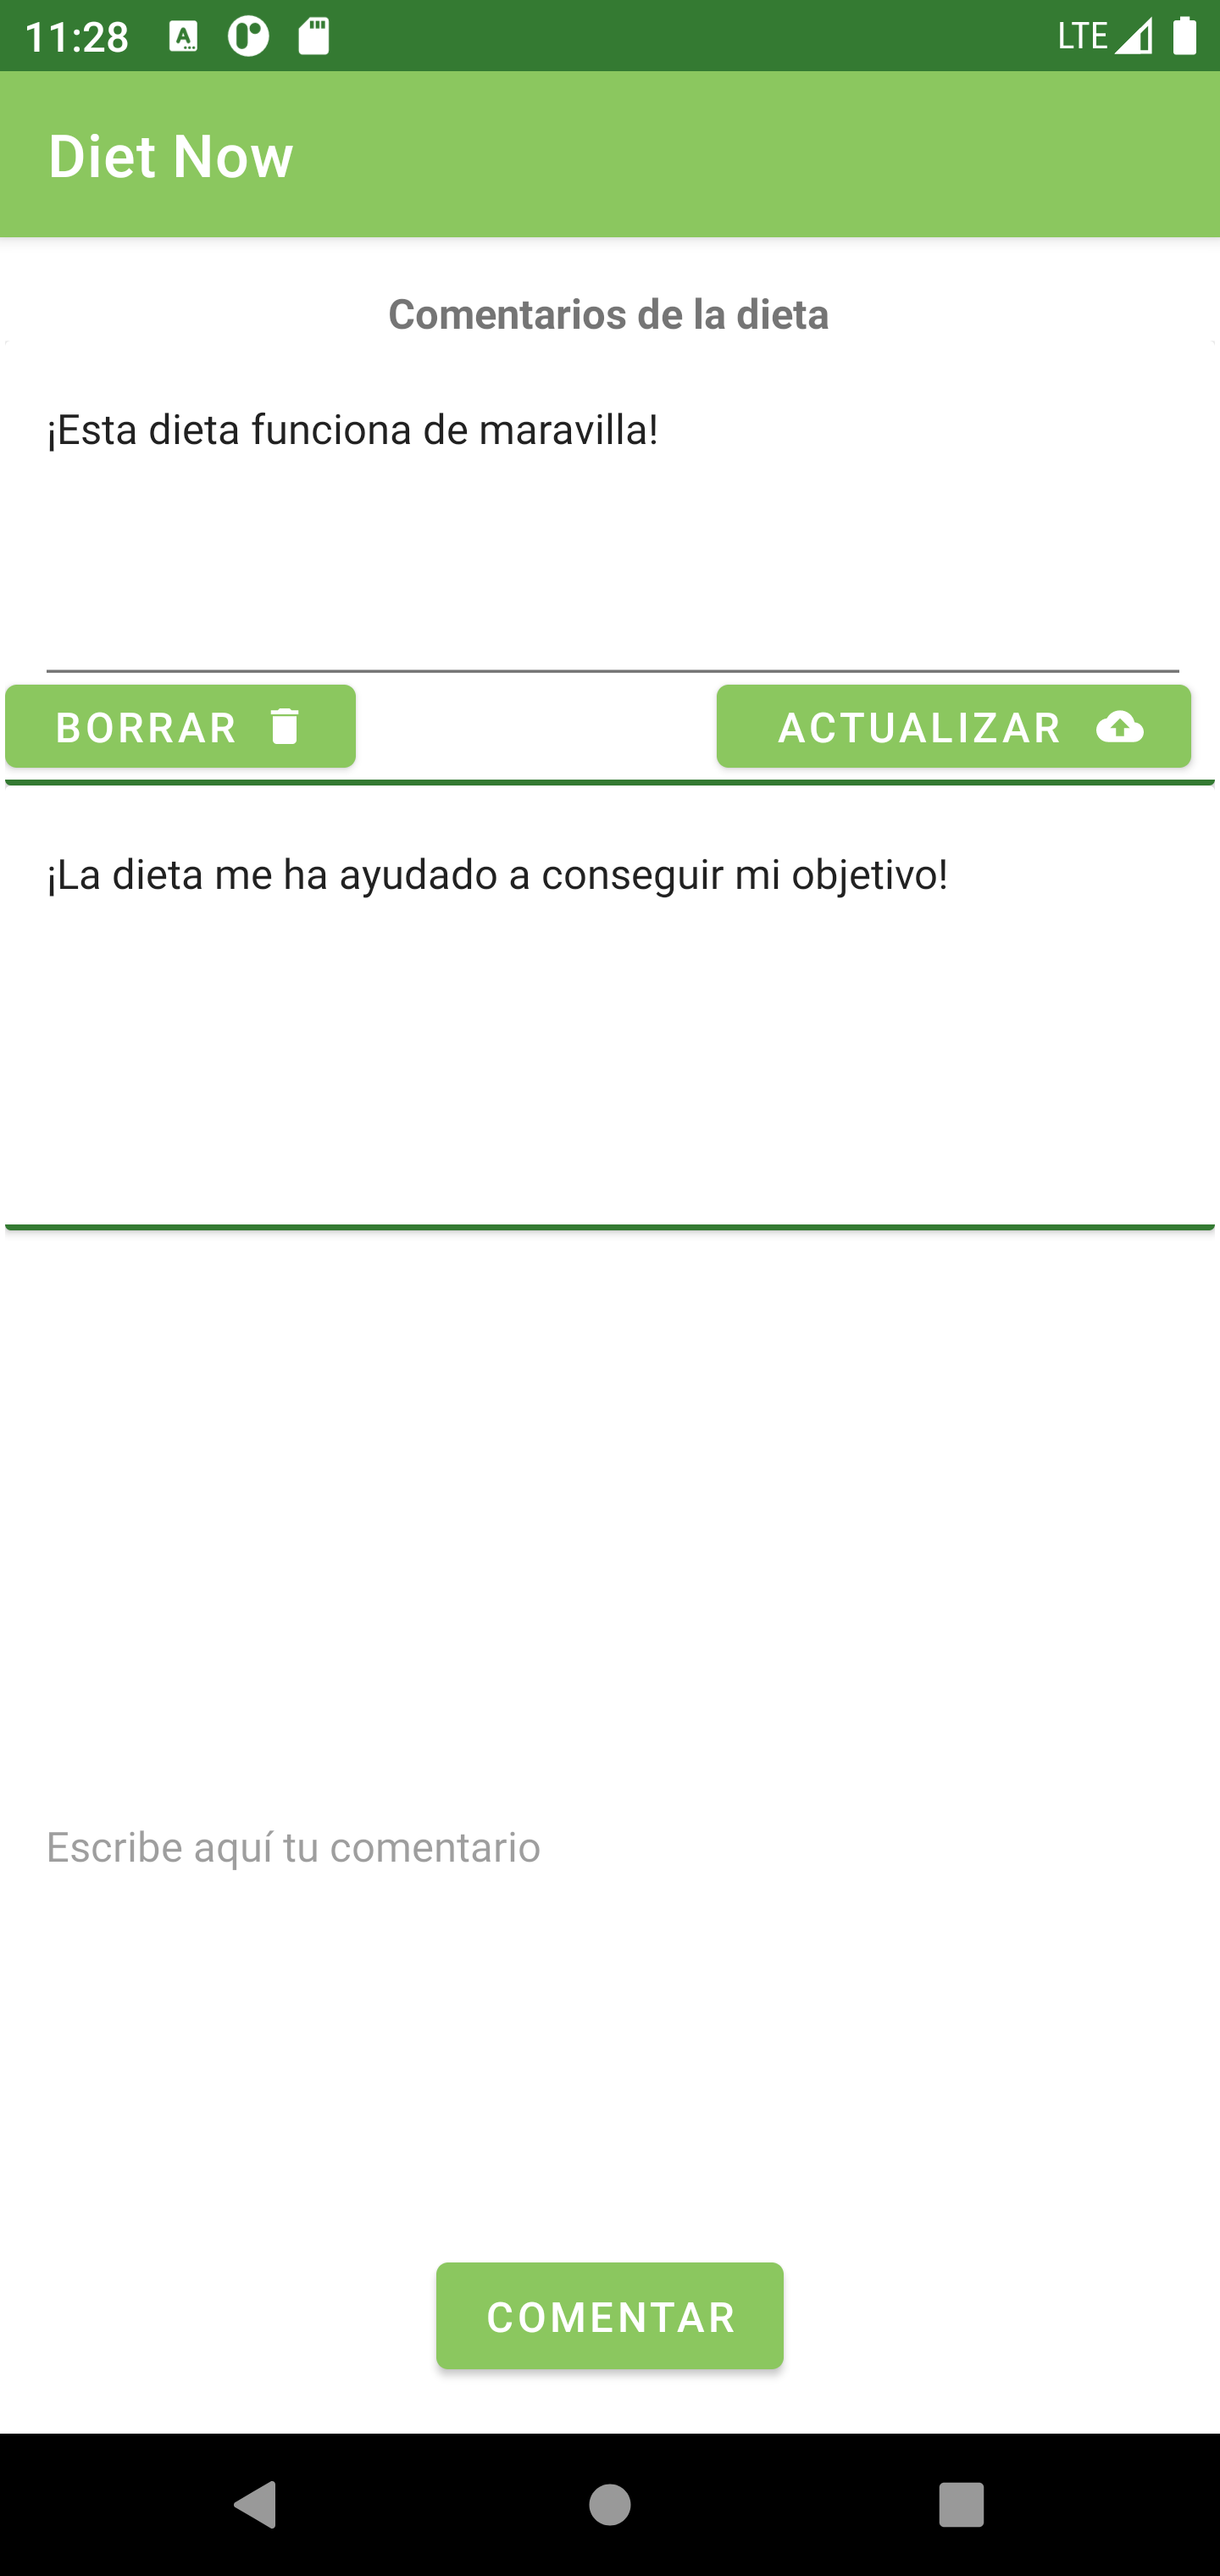
\includegraphics[width=0.3\textwidth]{Images/Annexes/vista_comentarios_dieta_seguida.png}}
    \caption{Vista dietas publicadas}
    \label{fig:dietas_publicadas}
\end{figure}


\subsection{Dieta seguida}
Si el usuario pulsa esta opción verá la dieta que está siguiendo, como se muestra en la figura \ref{fig:dieta_seguida}, y podrá registrar los alimentos y la cantidad que ha comido en el día actual, podrá ver lo que ingirió a lo largo de la semana y dejar su feedback sobre la dieta ya sea dejando un me gusta, un no me gusta o un comentario, también podrá dejar de seguir la dieta.

\begin{figure}[H]
    \centering
    \subfigure{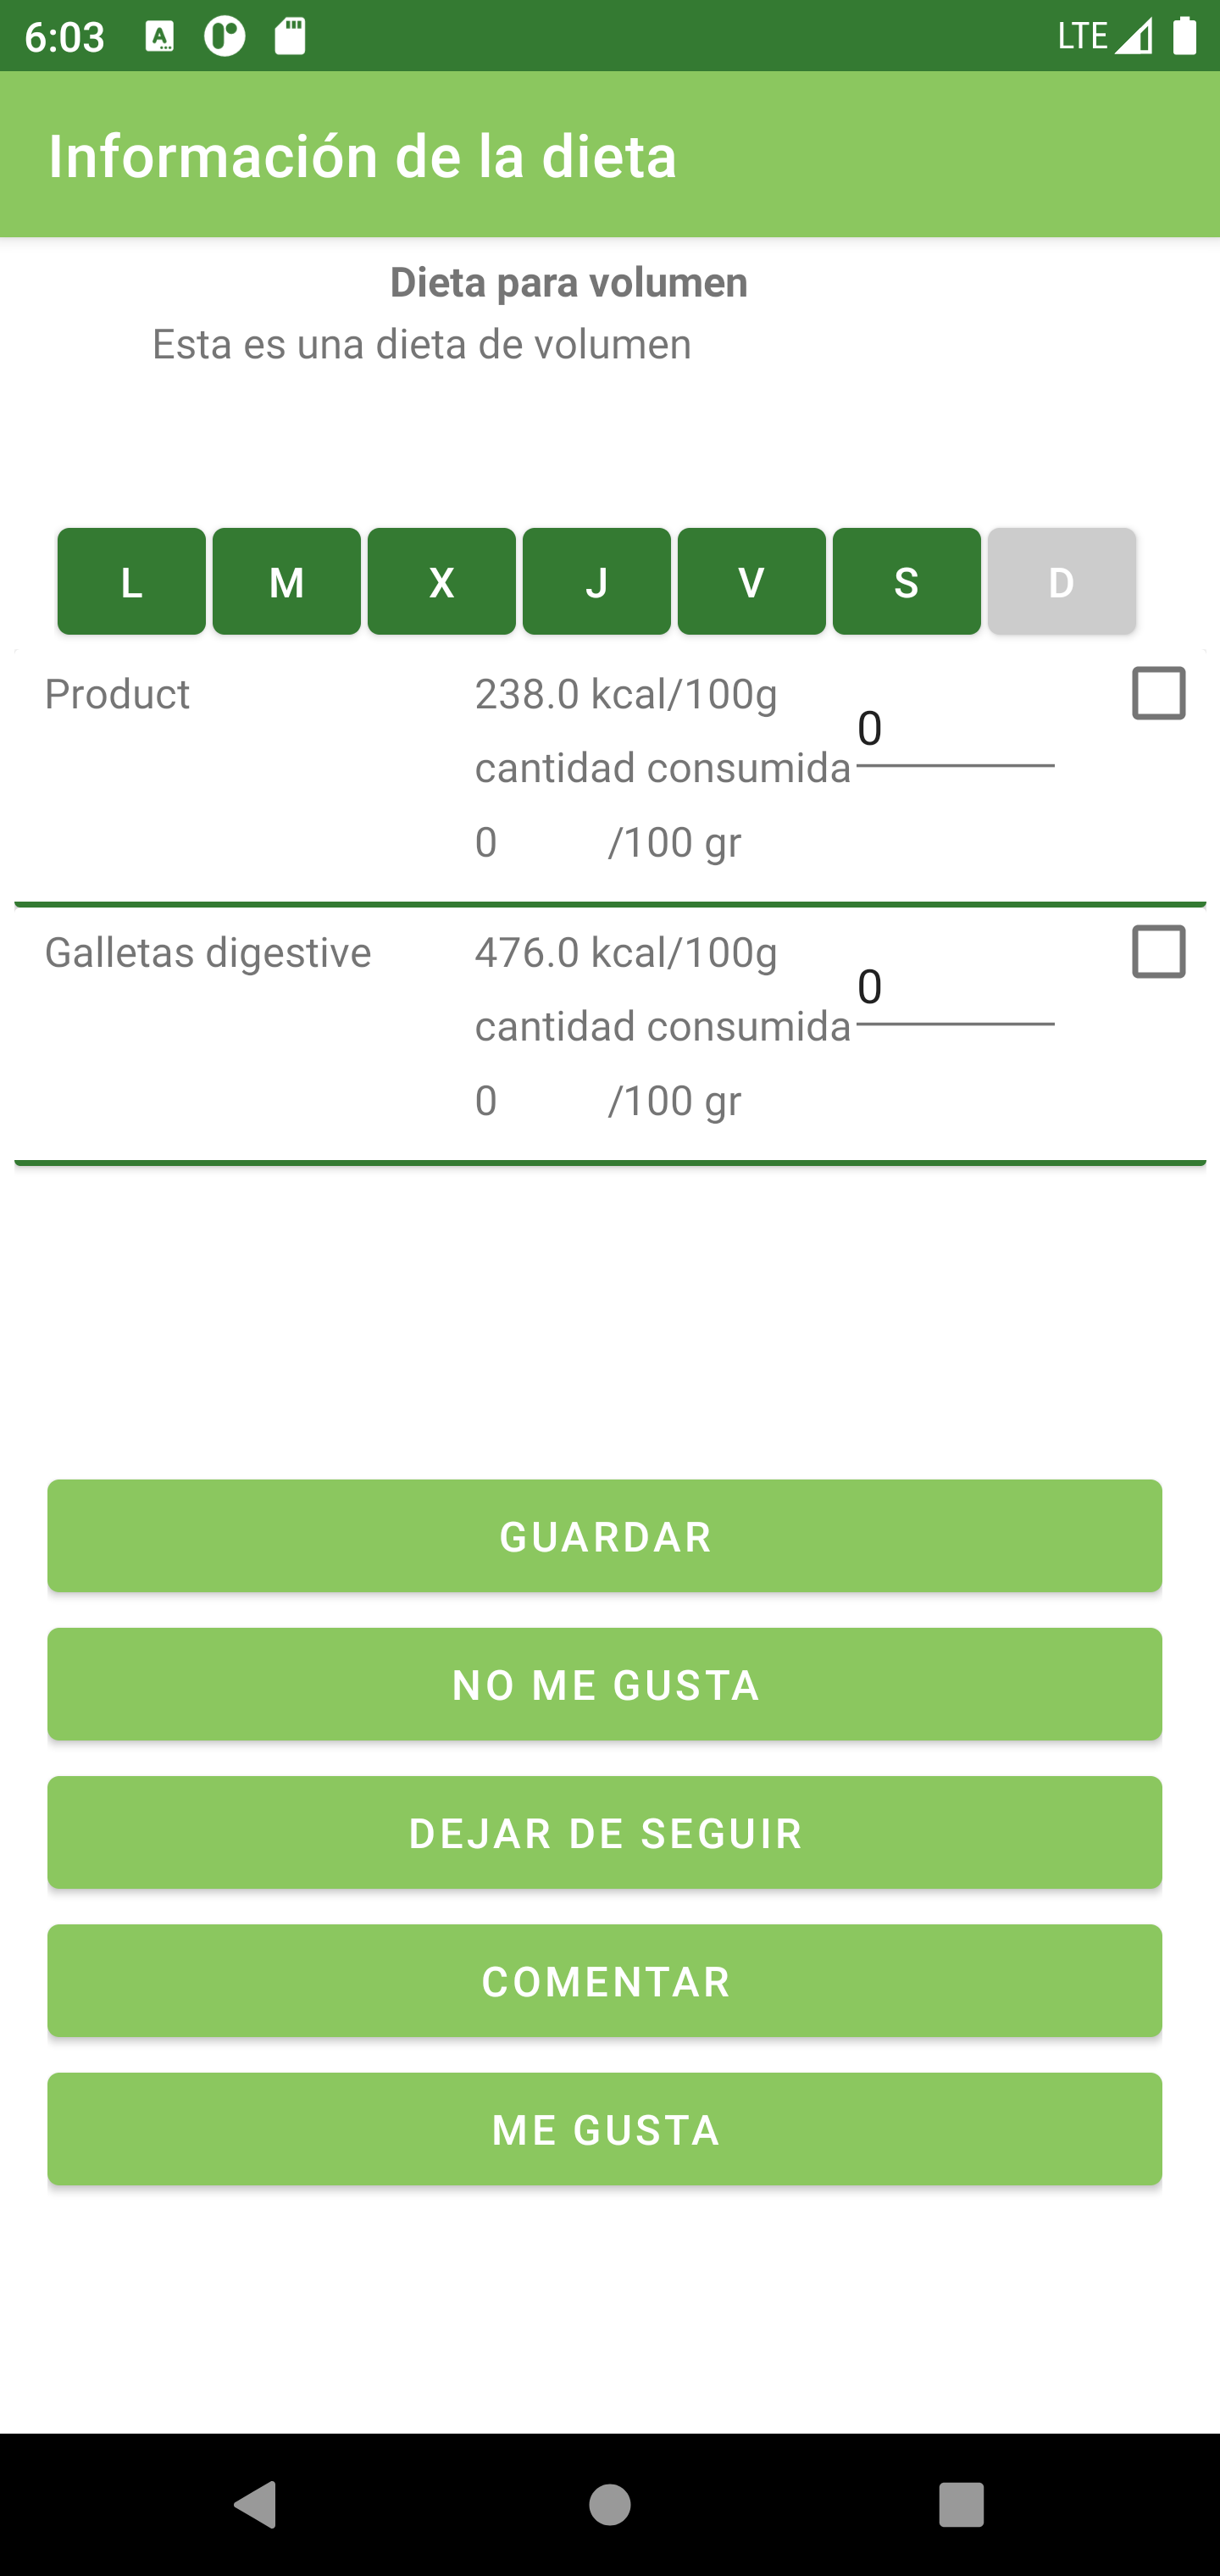
\includegraphics[width=0.4\textwidth]{Images/Annexes/dieta_seguida1.png}}
    \subfigure{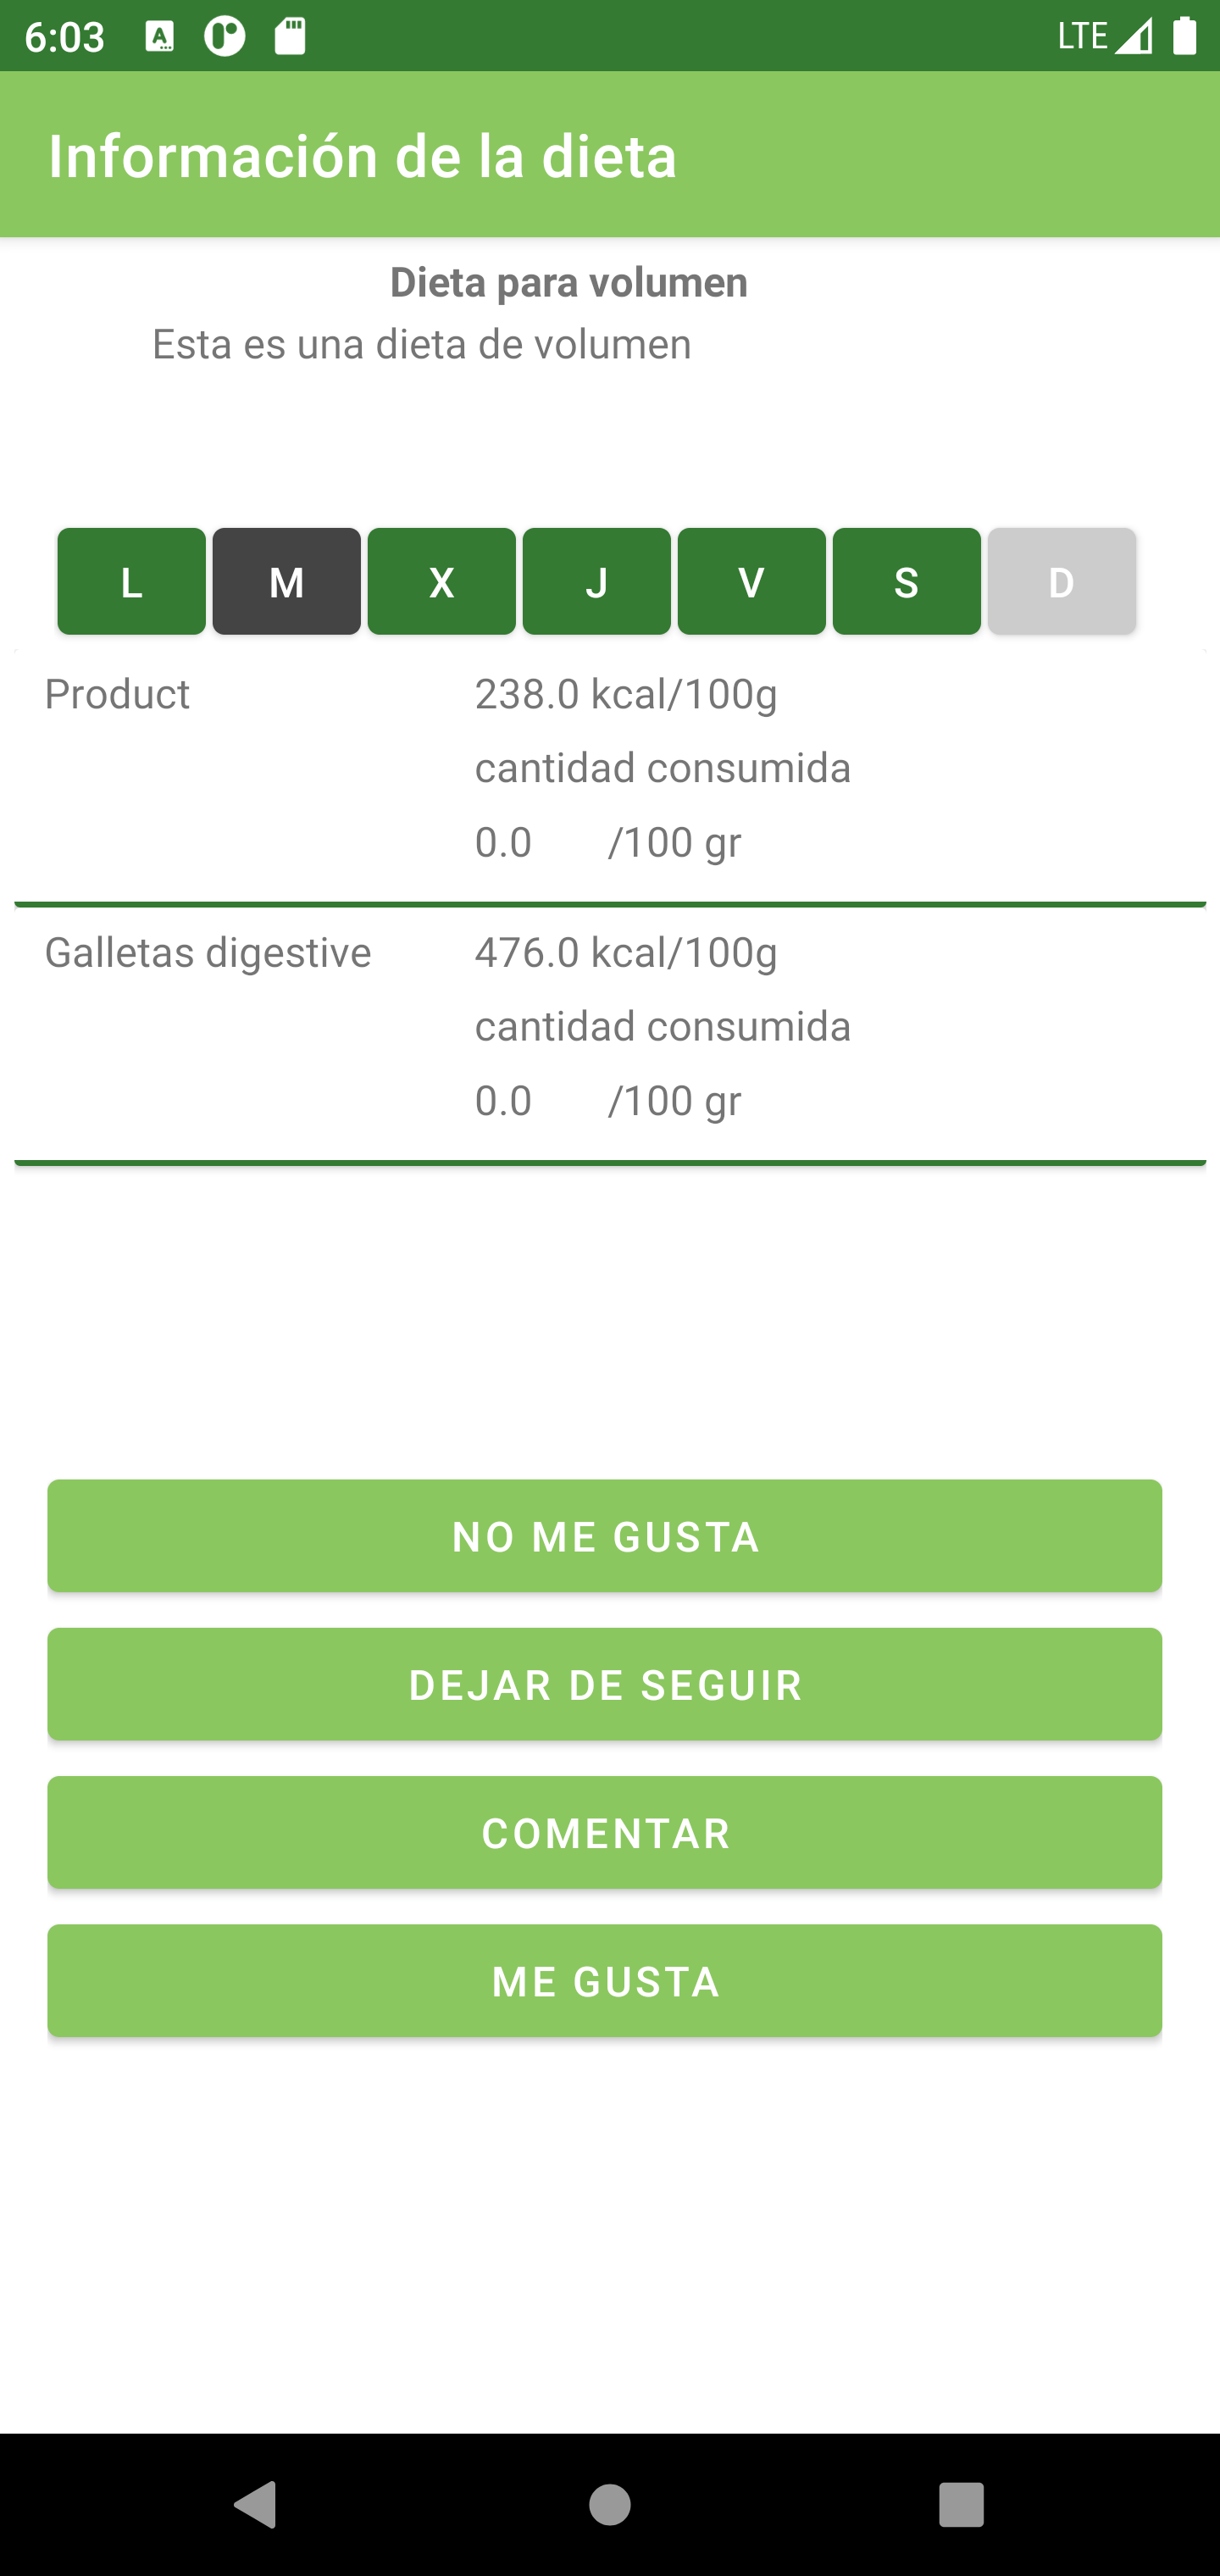
\includegraphics[width=0.4\textwidth]{Images/Annexes/dieta_seguida2.png}}
    \caption{Vista de dieta seguida}
    \label{fig:dieta_seguida}
\end{figure}

\subsection{Ver perfil}
Si se selecciona esta opción, el usuario será redirigido a una ventana que mostrará su información personal y las gráficas asociadas a él, como se puede apreciar en la Figura \ref{fig:user_profile}. Las acciones que puede realizar en esta vista son registrar pasos y/o peso del día actual, ver el historial de dietas seguidas, actualizar sus datos personales, cambiar la imagen de perfil, eliminar el perfil y cerrar sesión.

\begin{figure}[H]
    \centering
    \subfigure{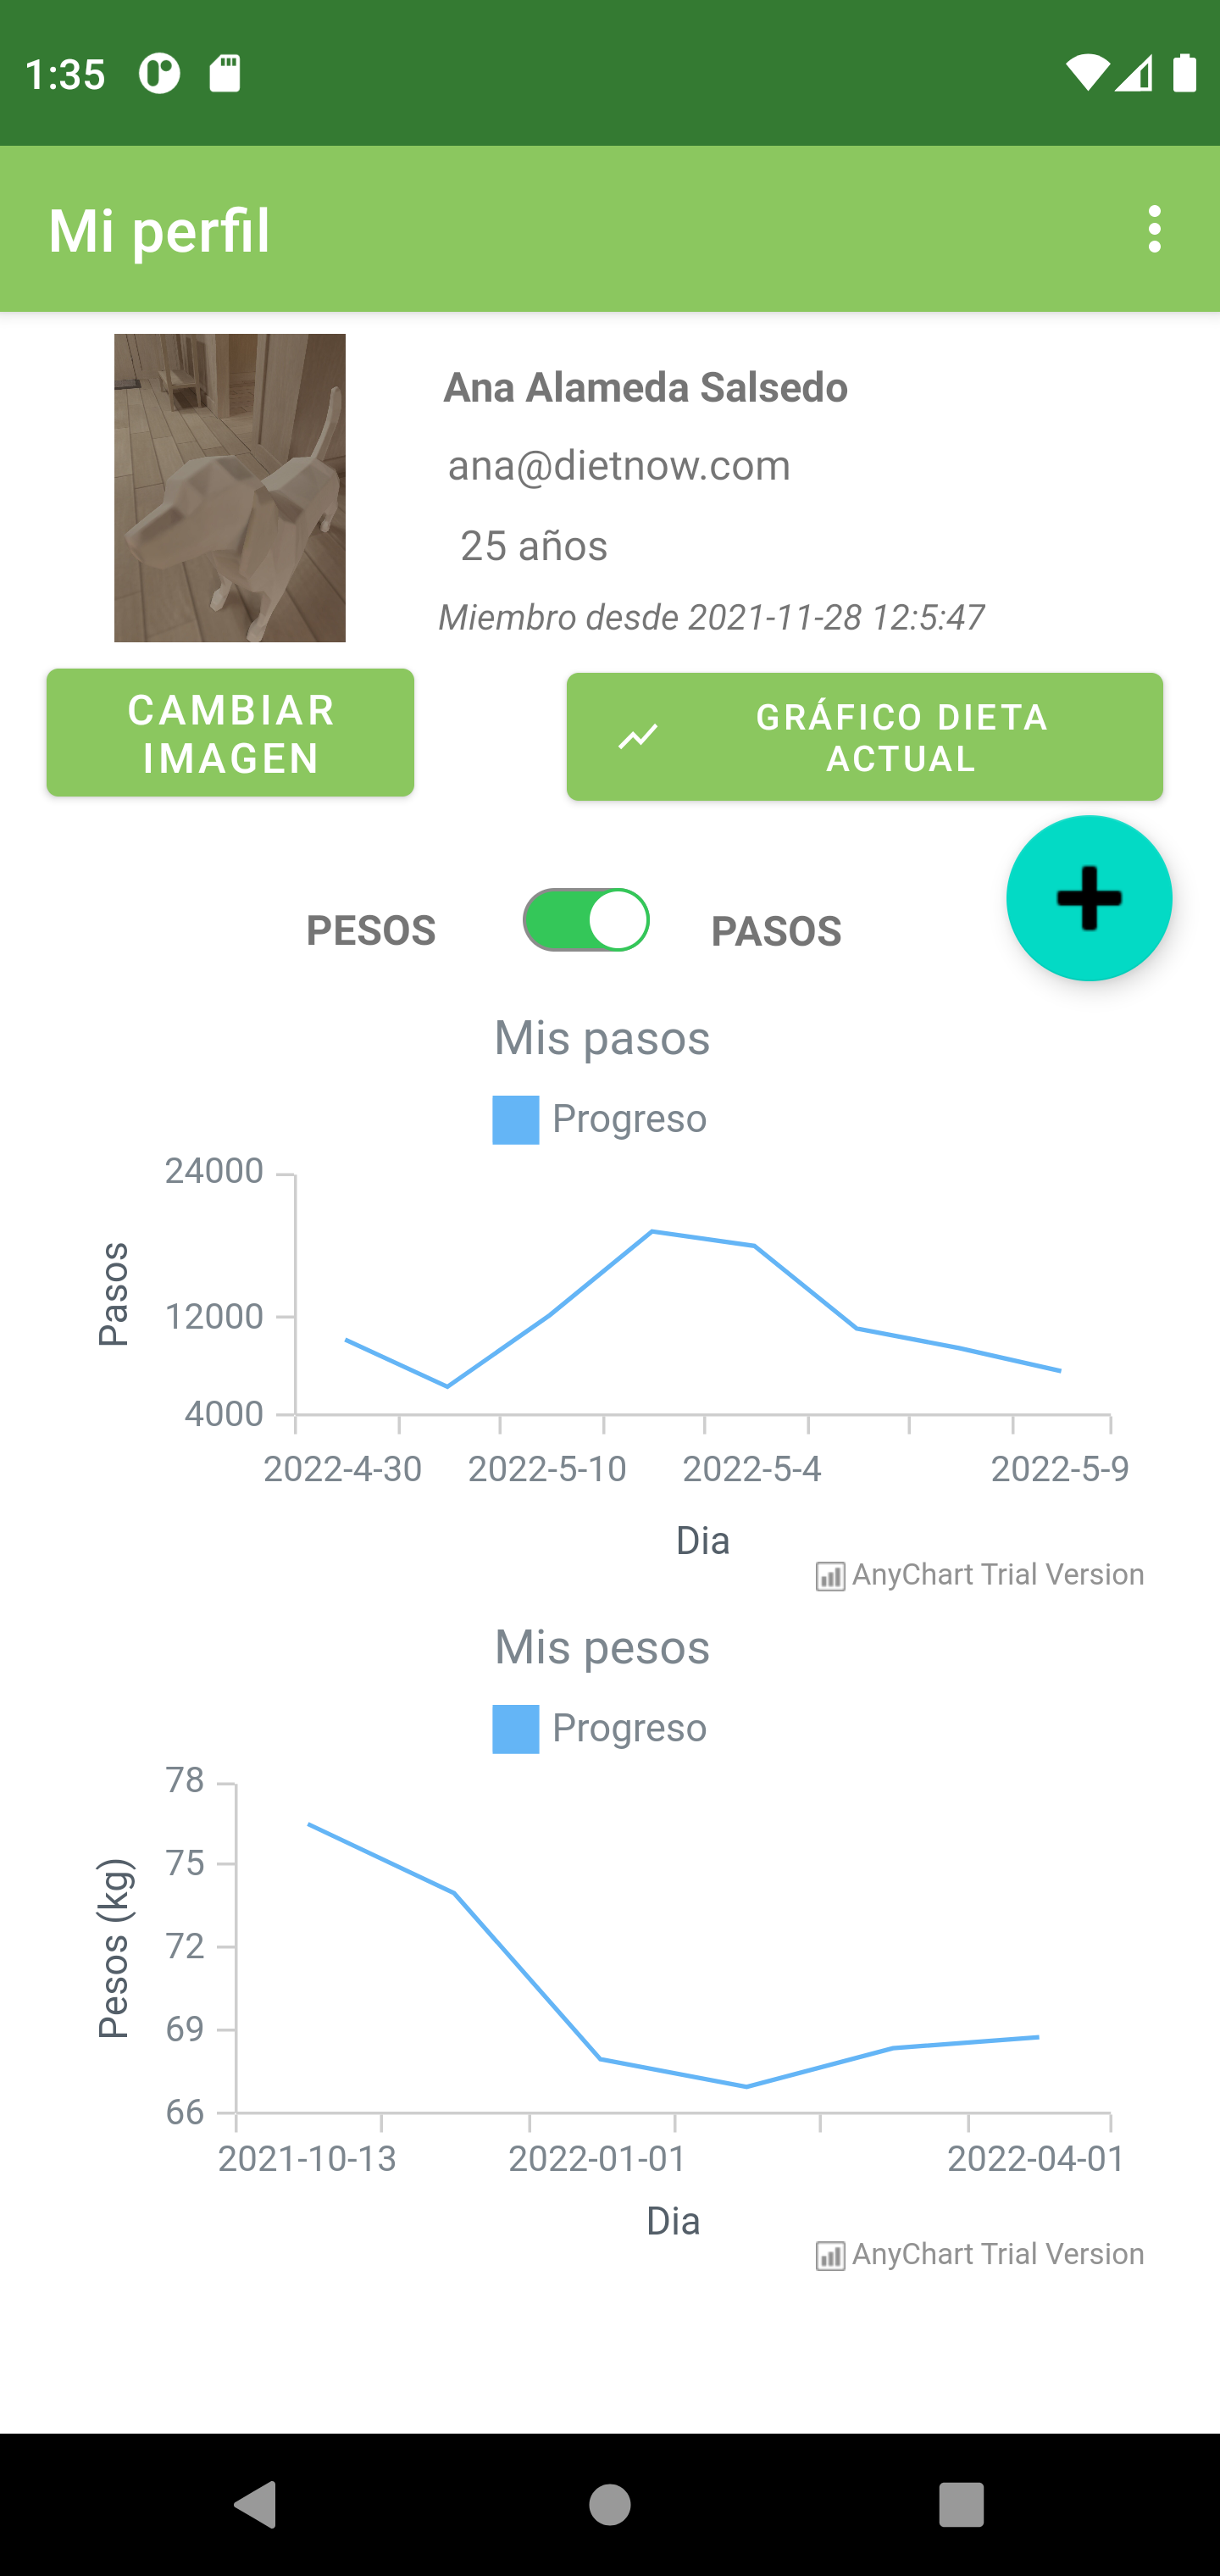
\includegraphics[width=0.4\textwidth]{Images/Annexes/userProfile.png}}
    \subfigure{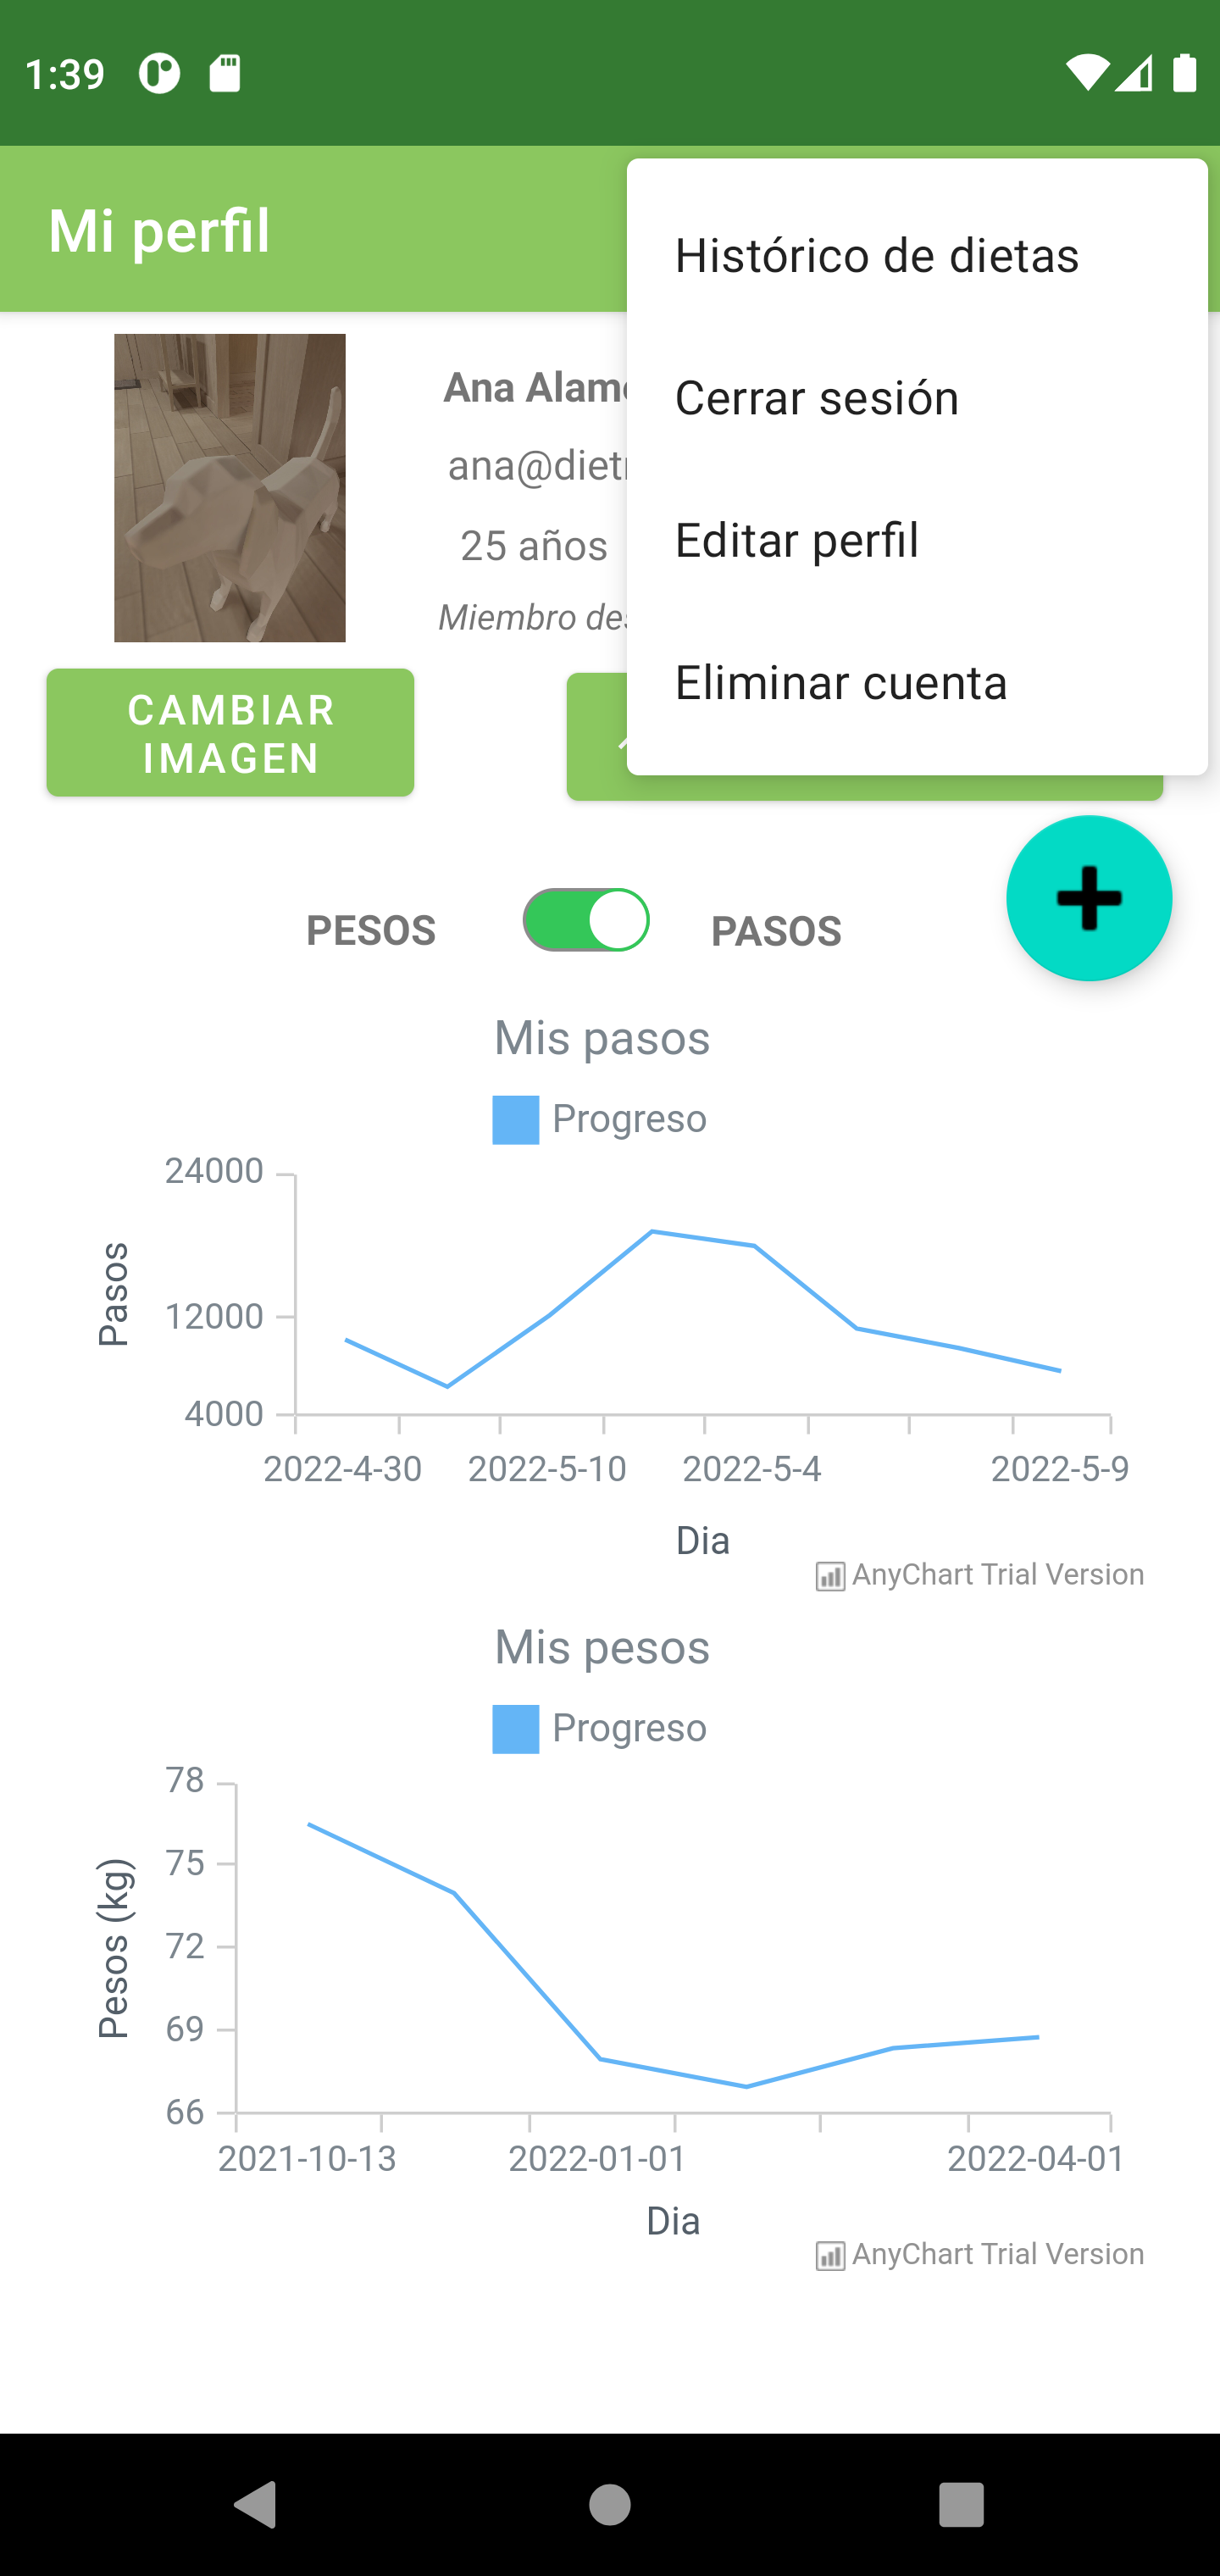
\includegraphics[width=0.4\textwidth]{Images/Annexes/userProfile2.png}}
    \caption{Vista del perfil de usuario}
    \label{fig:user_profile}
\end{figure}

%%%%%%%%%%%%%%%%%%%%%%%%%%%%%%%%%%%%%%%%%%%%%%%%%%%%%%%%%%%%

\section{Administradores}
Rol pensado para asegurar el correcto funcionamiento de la aplicación, algunas de las funciones de este rol son la gestión de usuarios, creación de dietas predeterminadas y control de contenido.

\subsection{Crear usuario}
Mediante esta opción se accede a un formulario similar al de registro de usuario, como se muestra en la figura \ref{fig:crear_usuario_admin}, donde el administrador puede crear una cuenta, la diferencia respecto al formulario de registro es que mientras que en el formulario de registro la cuenta creada siempre tendrá rol usuario, en crear cuenta el administrador puede decidir el rol de la cuenta que está creando.

\begin{figure}[H]
    \centering
    \subfigure{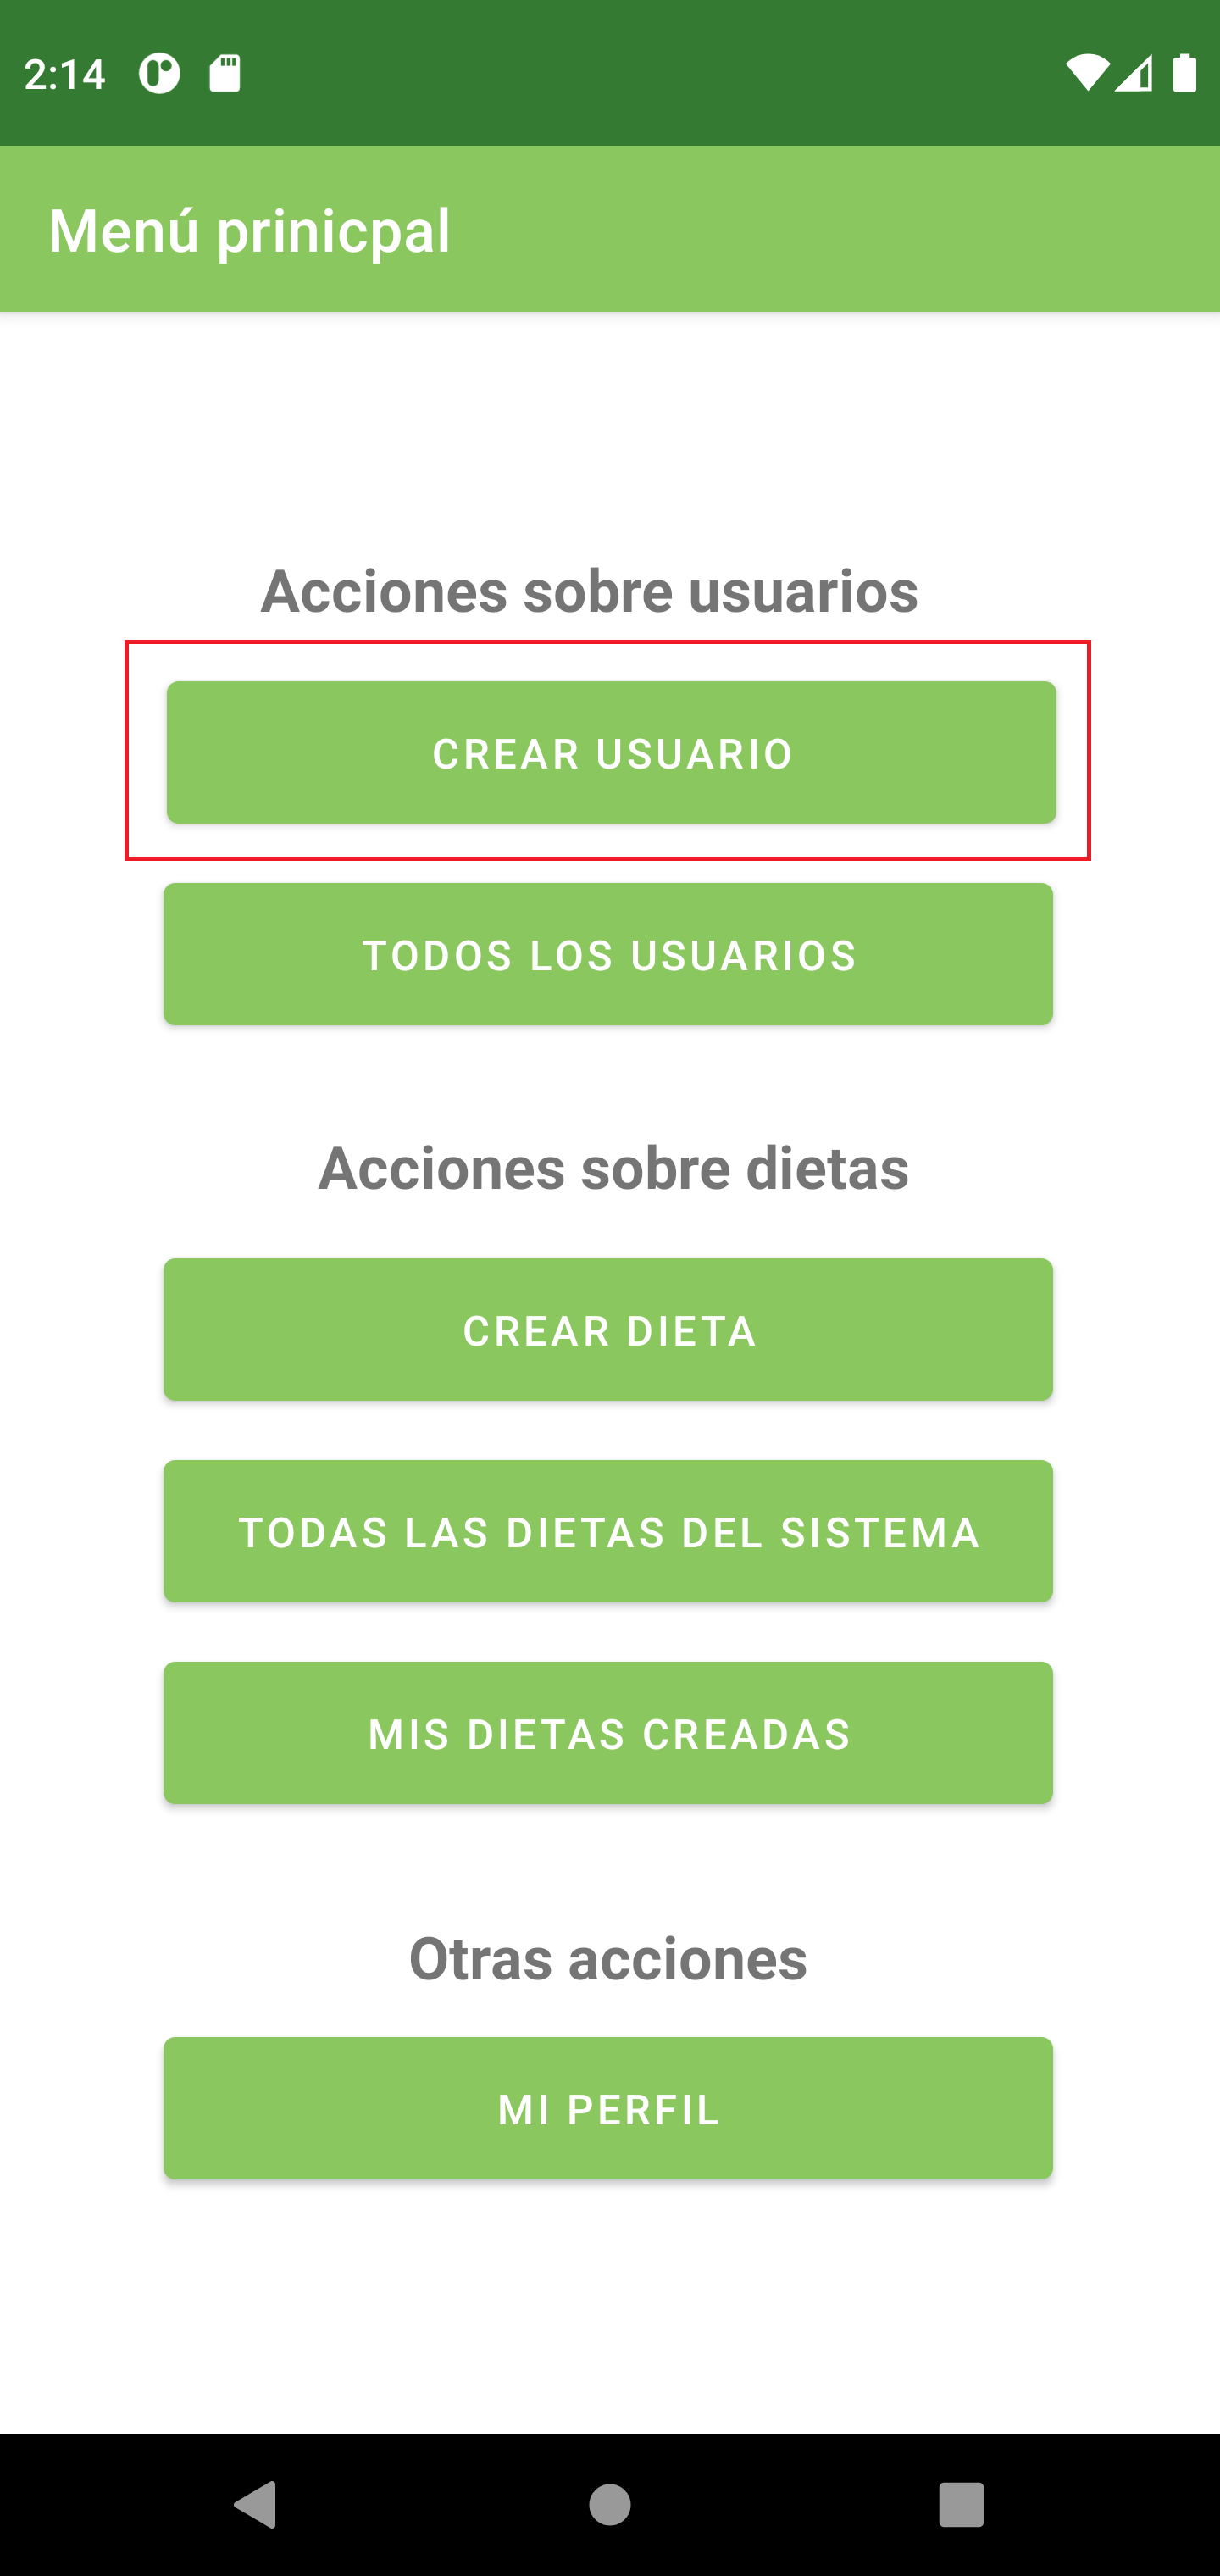
\includegraphics[width=0.4\textwidth]{Images/Annexes/createUsers.png}}
    \subfigure{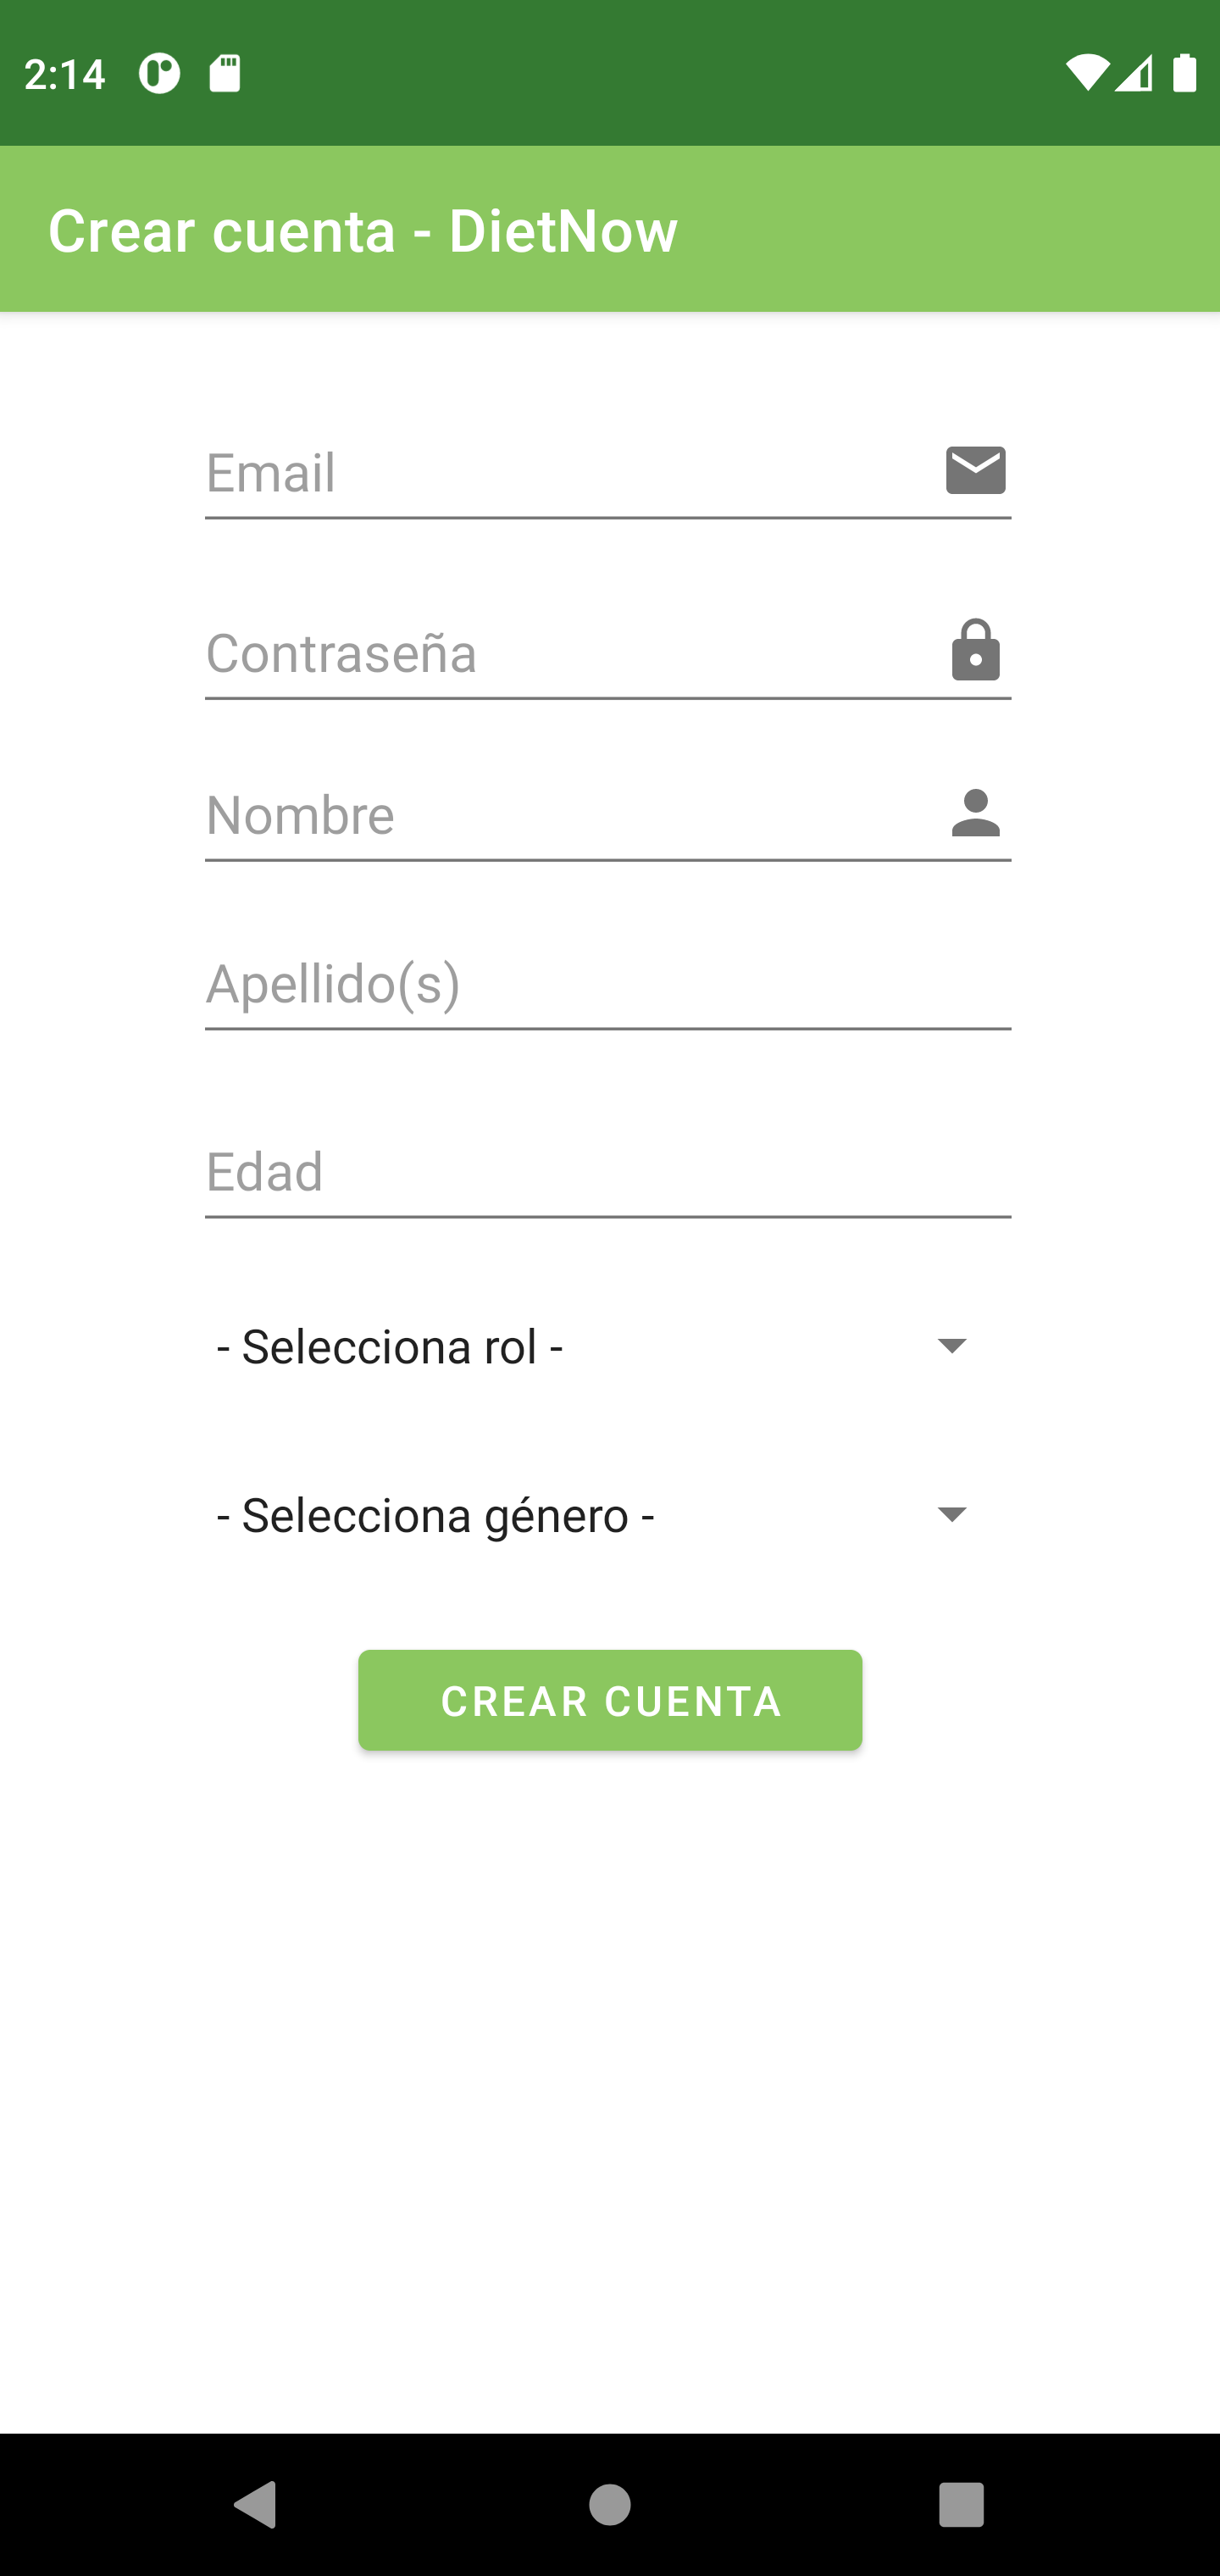
\includegraphics[width=0.4\textwidth]{Images/Annexes/createUsers2.png}}
    \caption{Creación de un usuario en la aplicación}
    \label{fig:crear_usuario_admin}
\end{figure}


\subsection{Todos los usuarios}
Si el administrador selecciona esta opción se abrirá en una nueva ventana un listado con todos los usuarios que están dados de alta en la aplicación, como se muestra en la figura \ref{fig:todos_usuarios}. En esta pantalla se puede filtrar dinámicamente a los usuarios mediante la lupa de la parte superior y se puede editar o eliminar a los diferentes usuarios de la aplicación.

\begin{figure}[H]
    \centering
    \subfigure{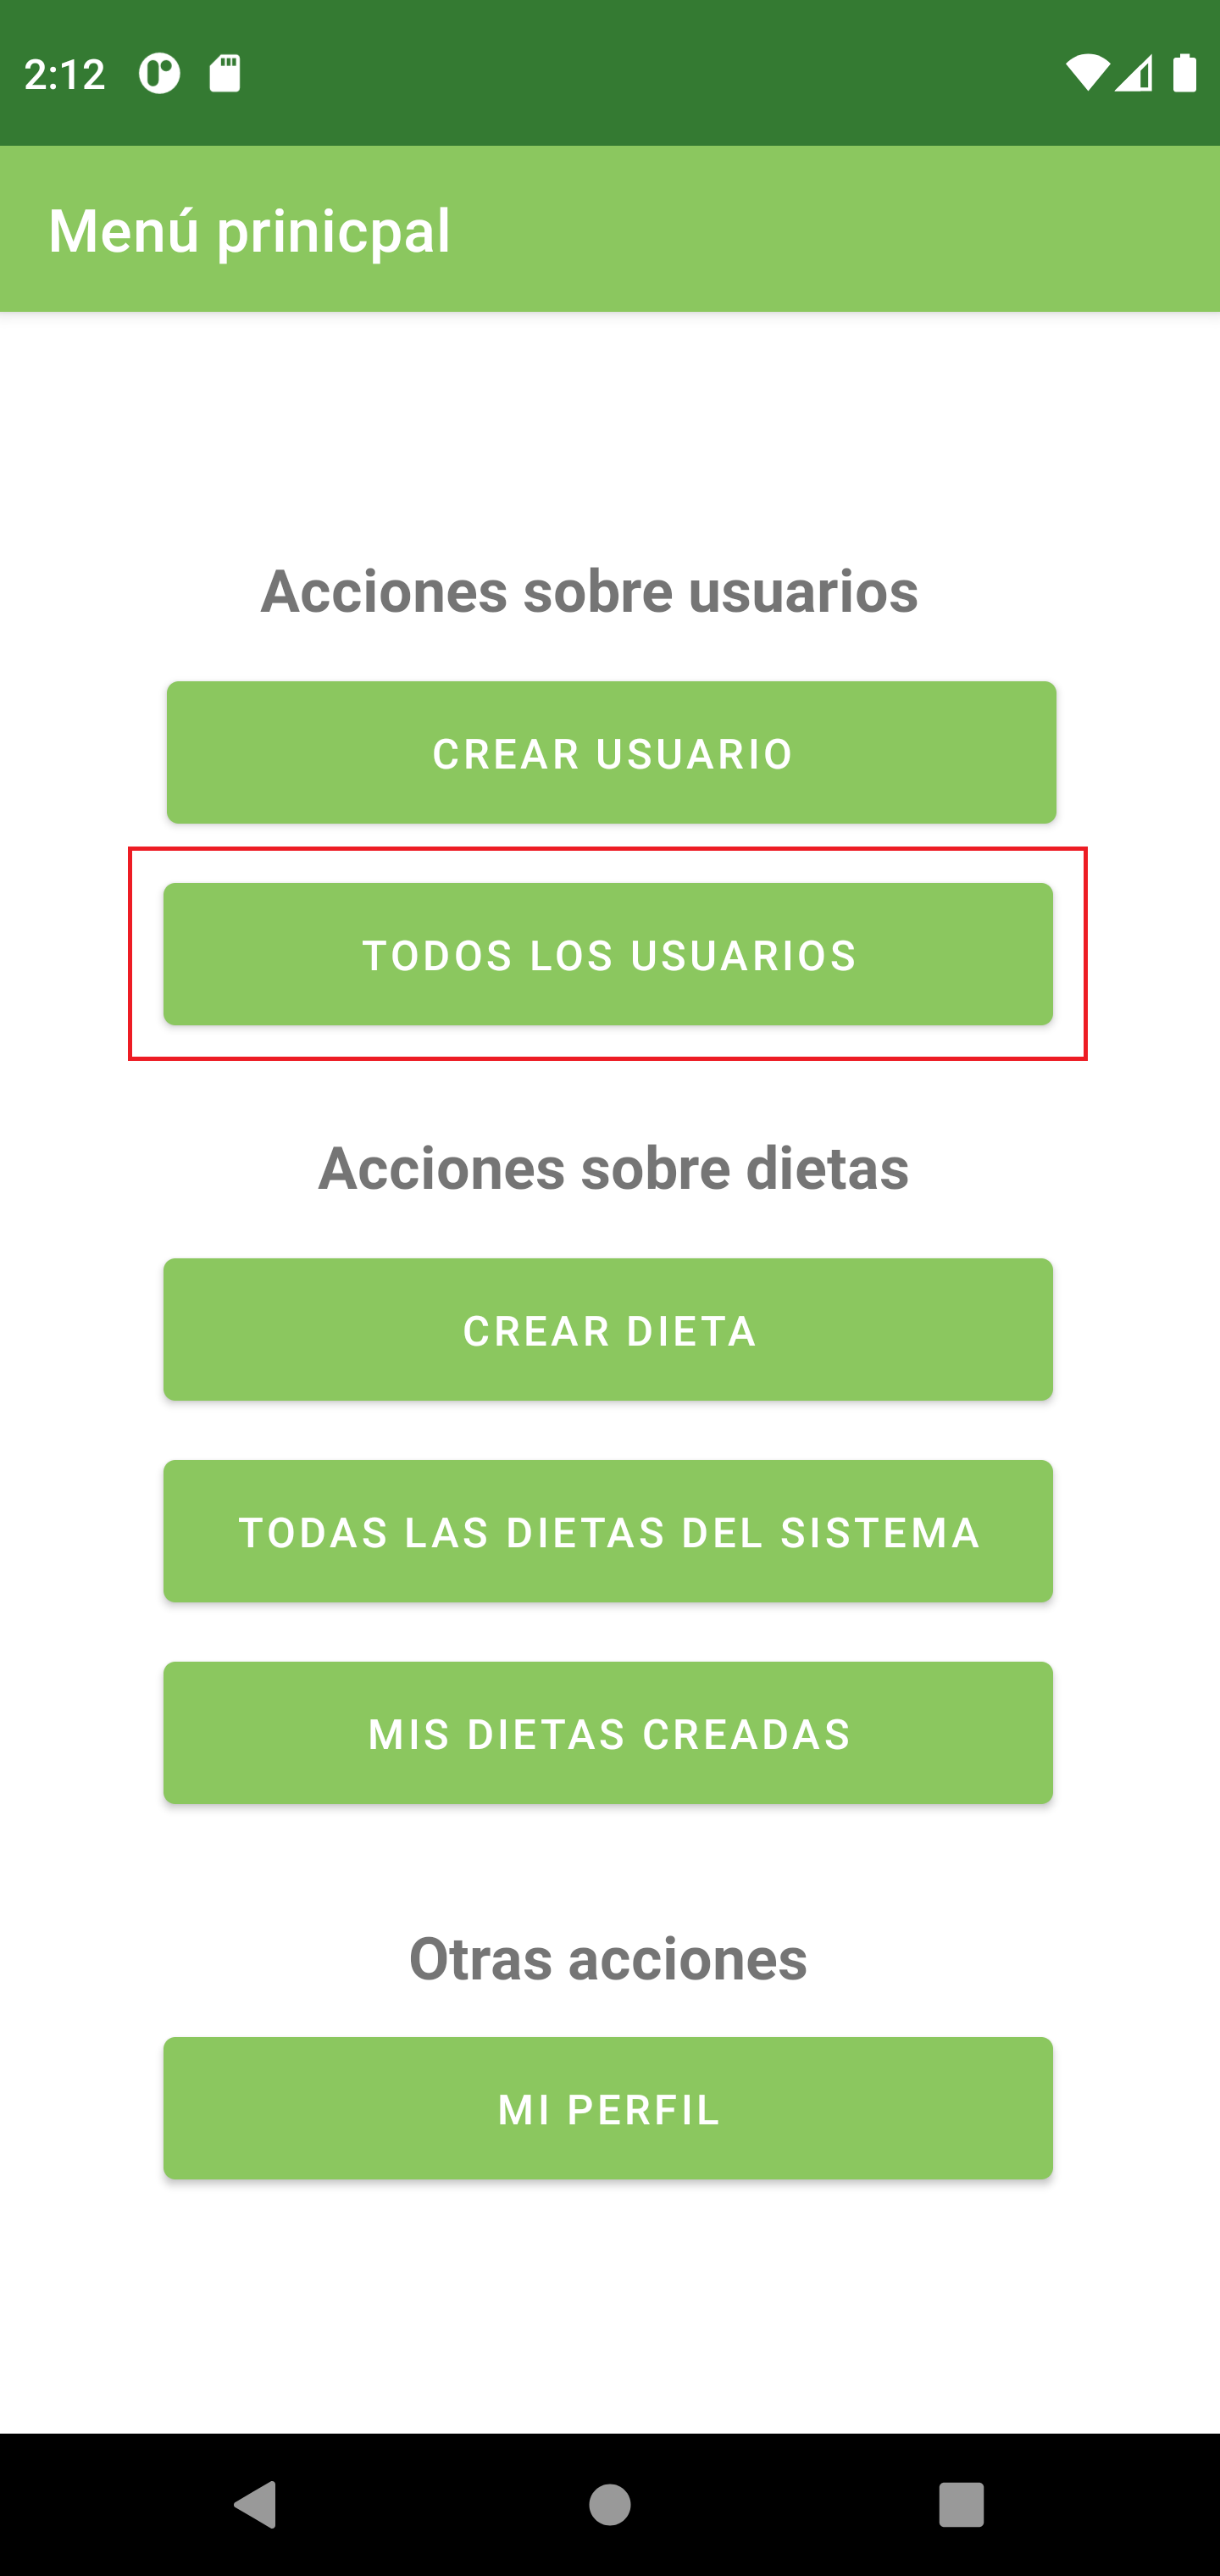
\includegraphics[width=0.4\textwidth]{Images/Annexes/allUsersAdmin.png}}
    \subfigure{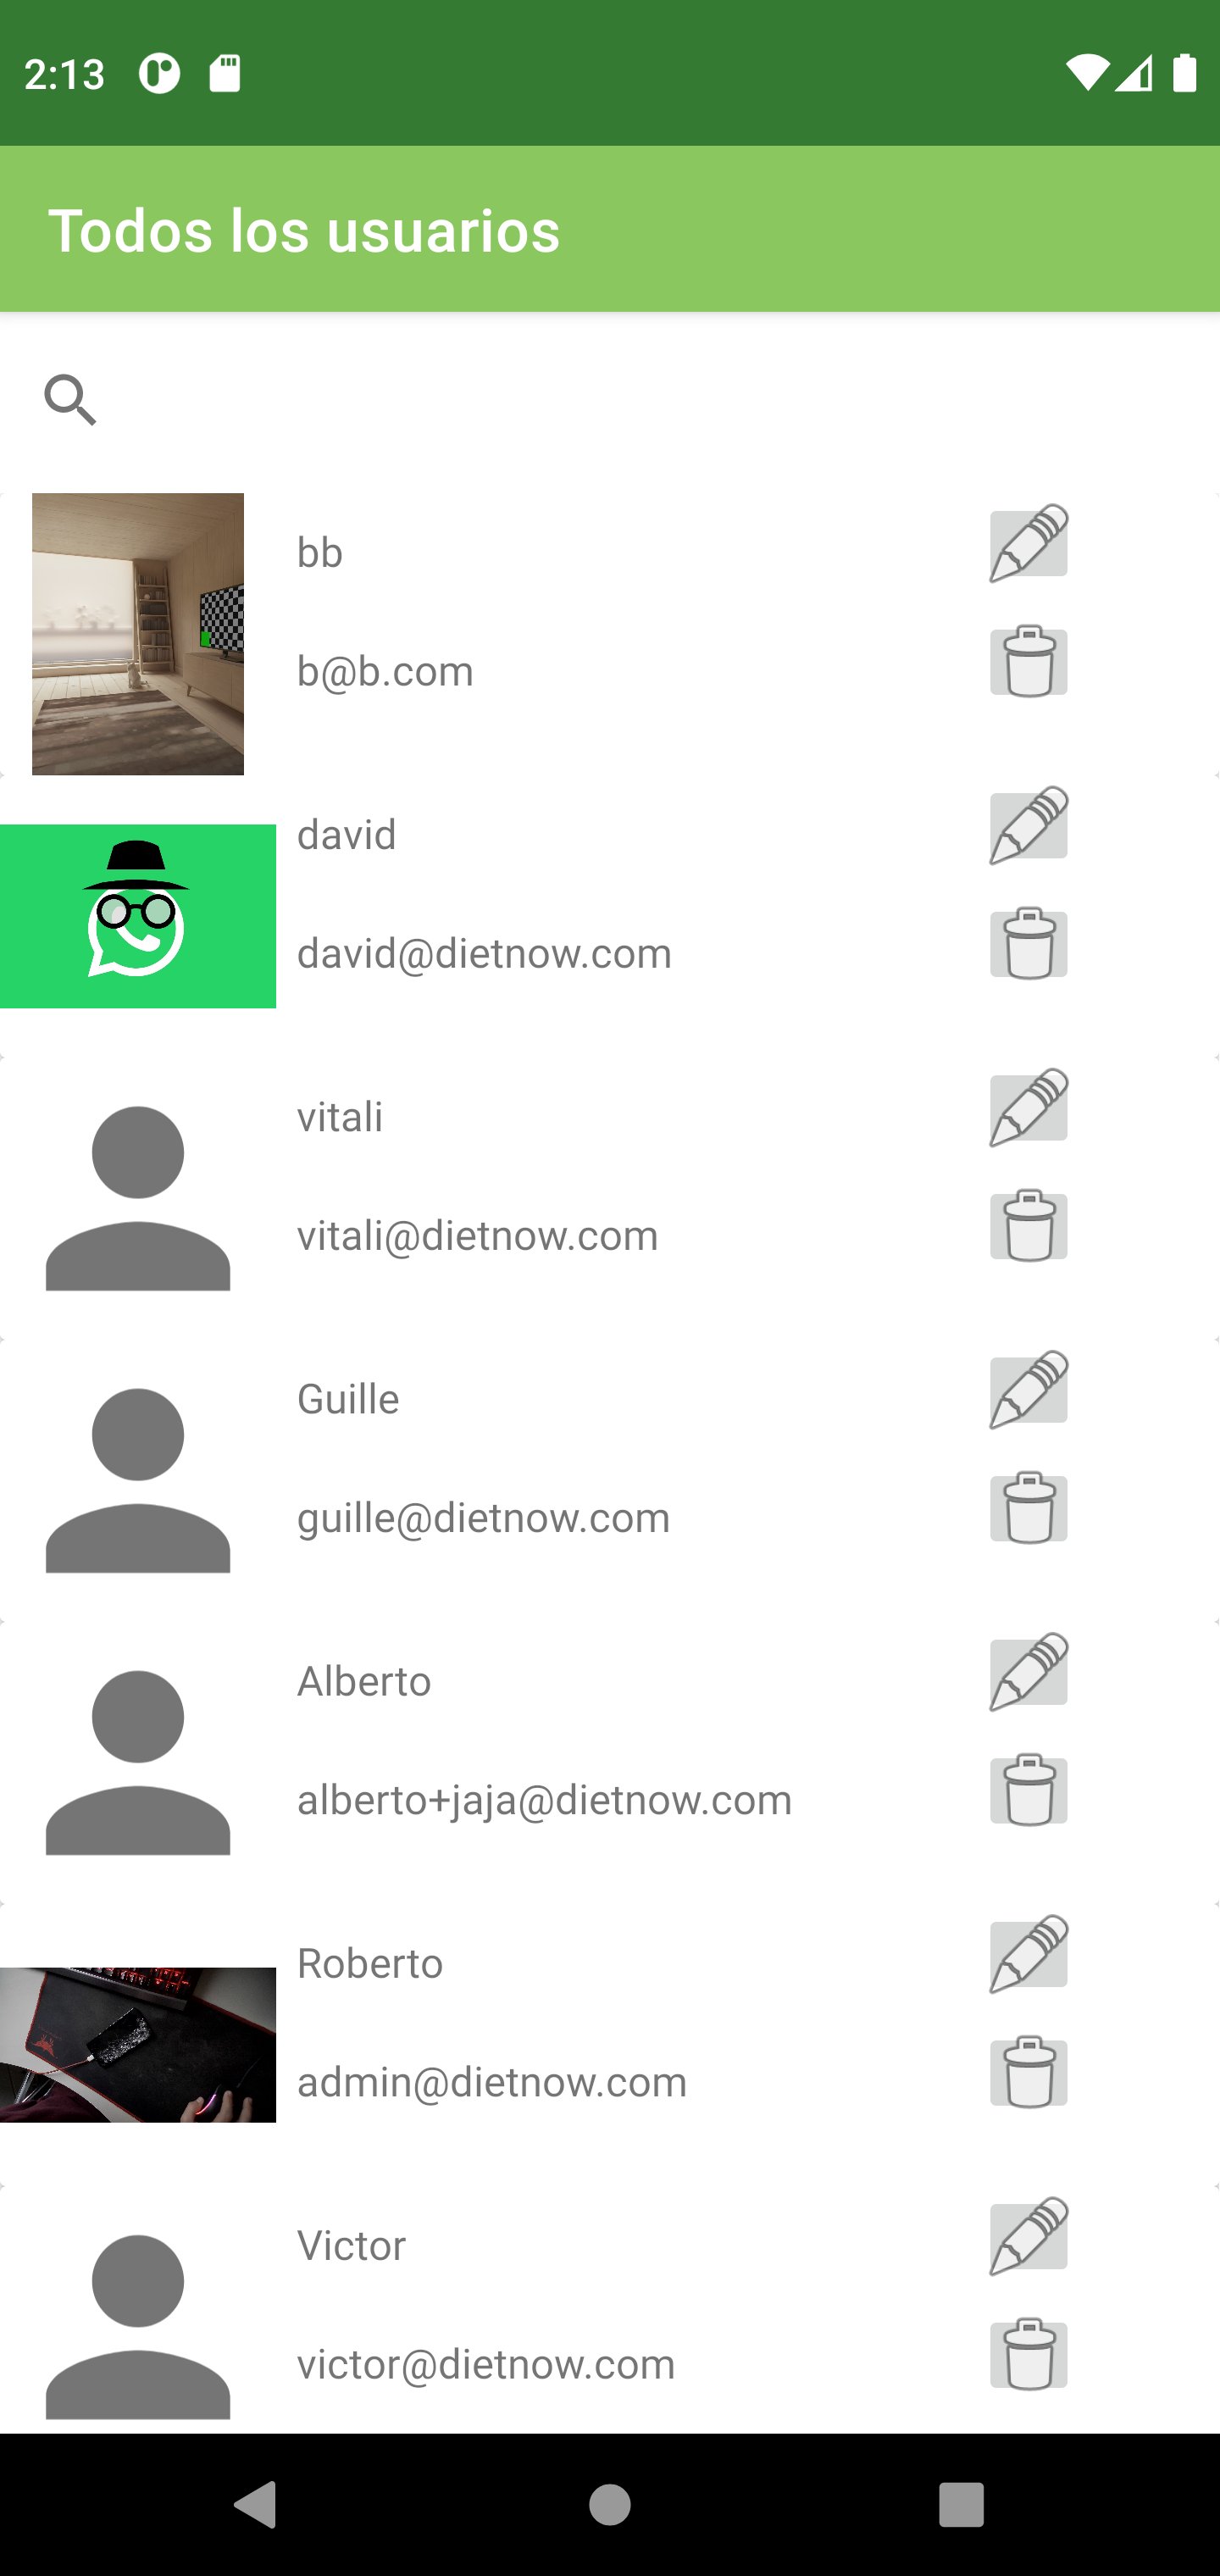
\includegraphics[width=0.4\textwidth]{Images/Annexes/allUsersAdmin2.png}}
    \caption{Vista de todos los usuarios}
    \label{fig:todos_usuarios}
\end{figure}


\subsection{Crear dieta}
Esta opción abre el formulario de creación de dieta, como se muestra en la figura \ref{fig:crear_dieta}, idéntico a cuando en el módulo ``Mis dietas creadas`` un usuario pulsa el botón circular con el símbolo ``$+$``.

\begin{figure}[H]
    \centering
    \subfigure{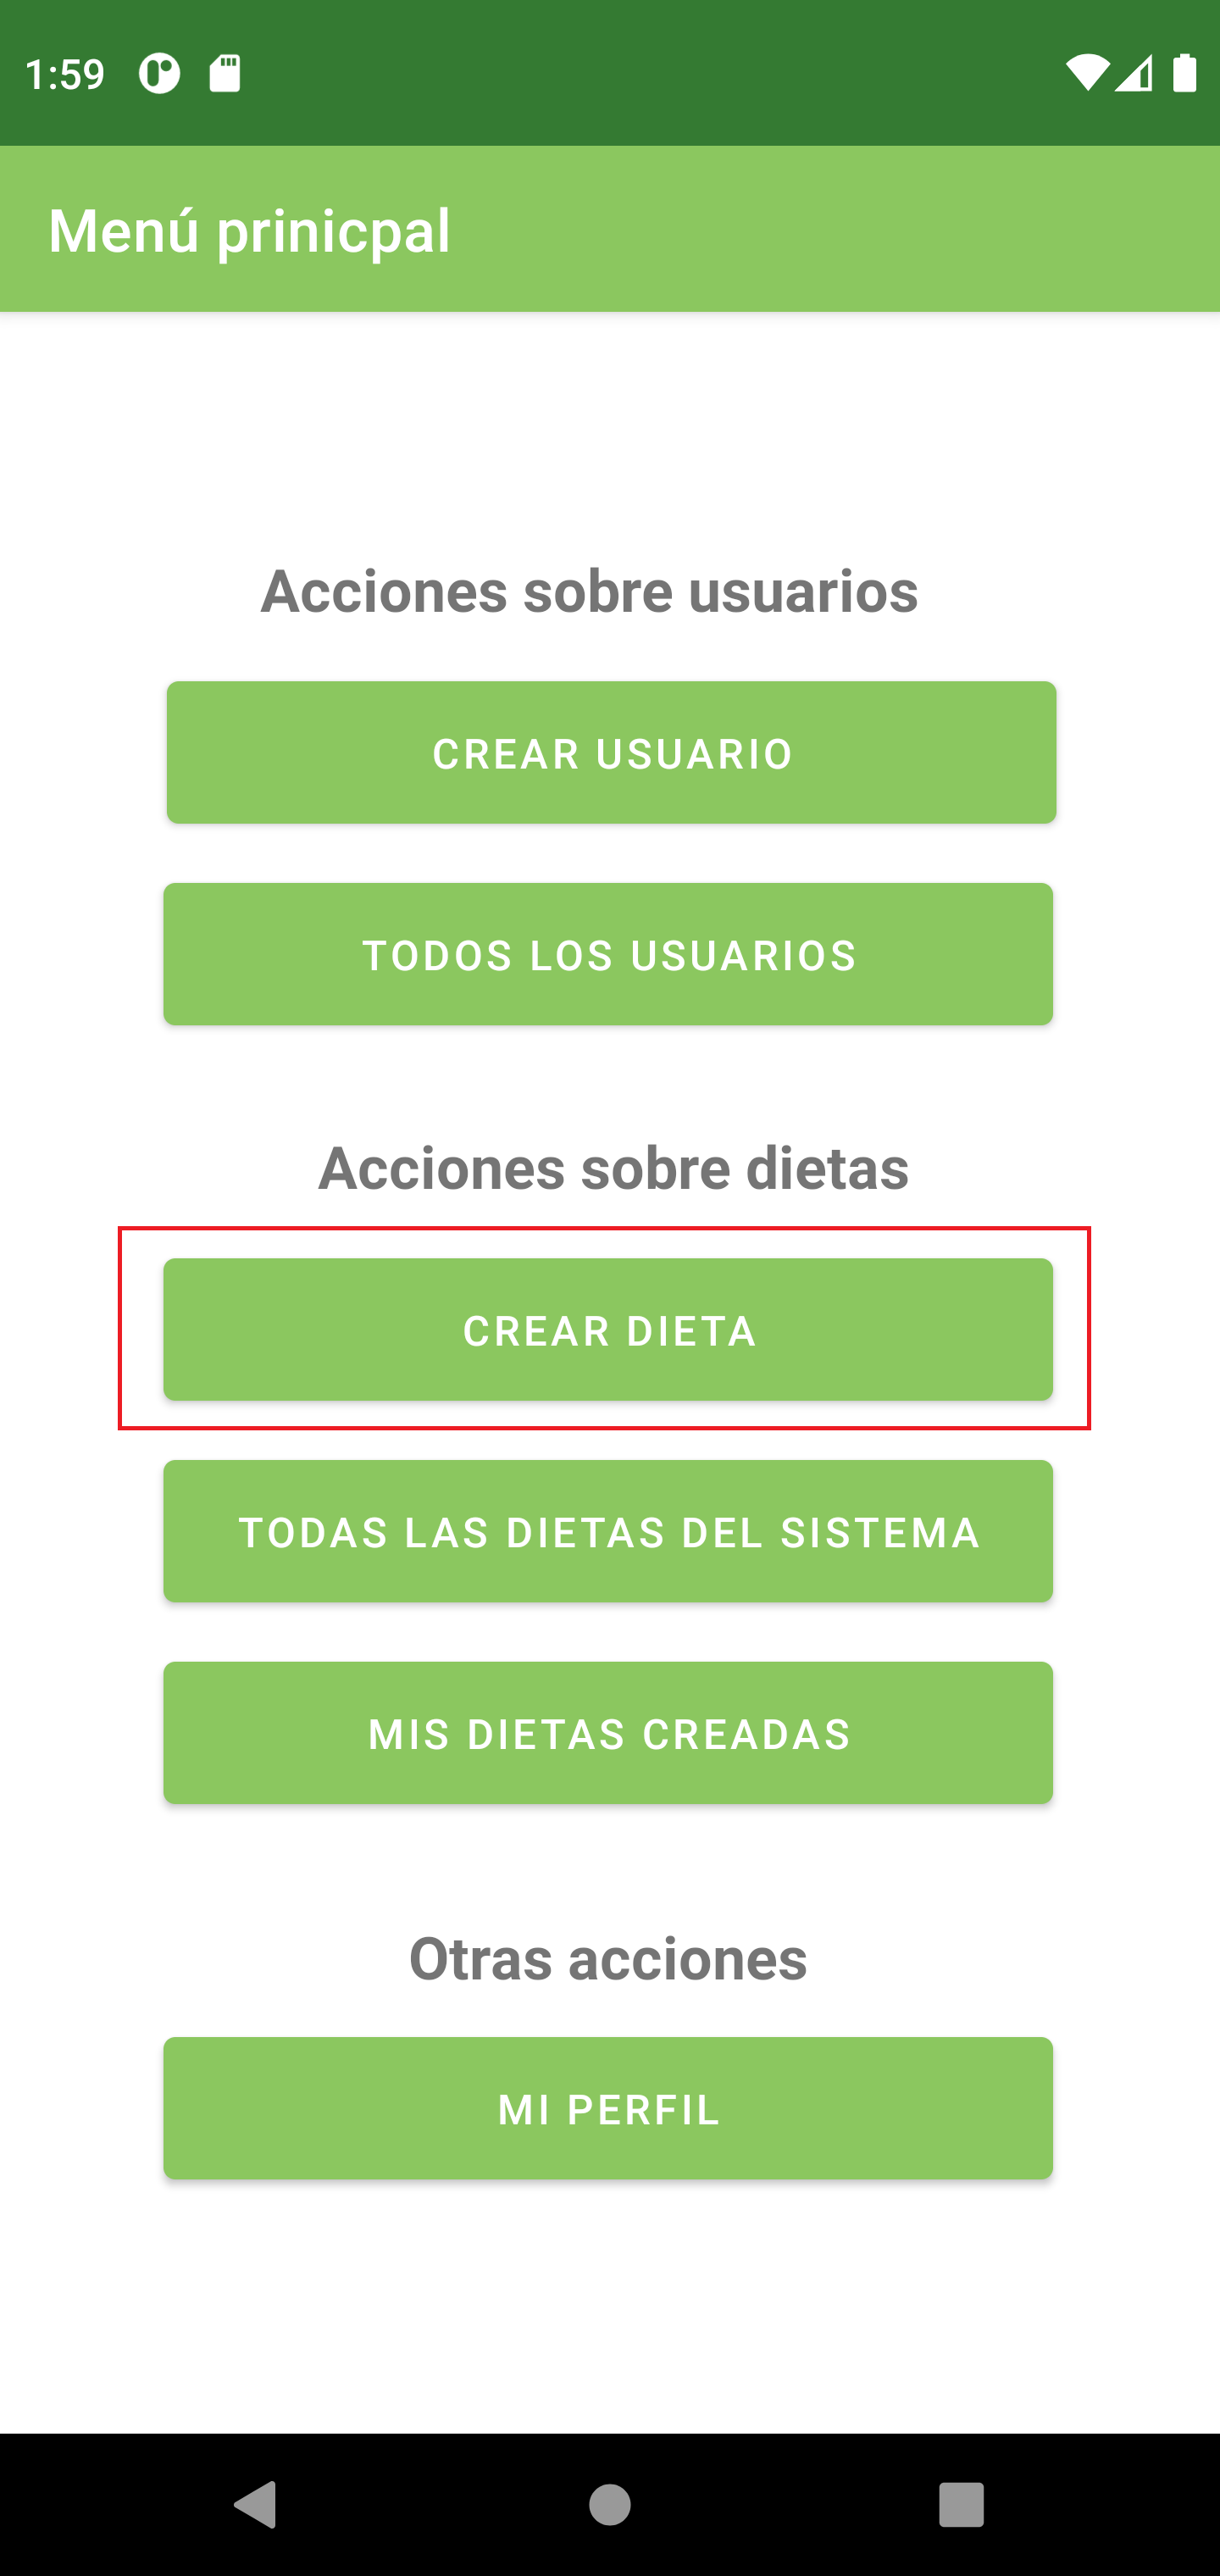
\includegraphics[width=0.4\textwidth]{Images/Annexes/adminCreateDiet.png}}
    \subfigure{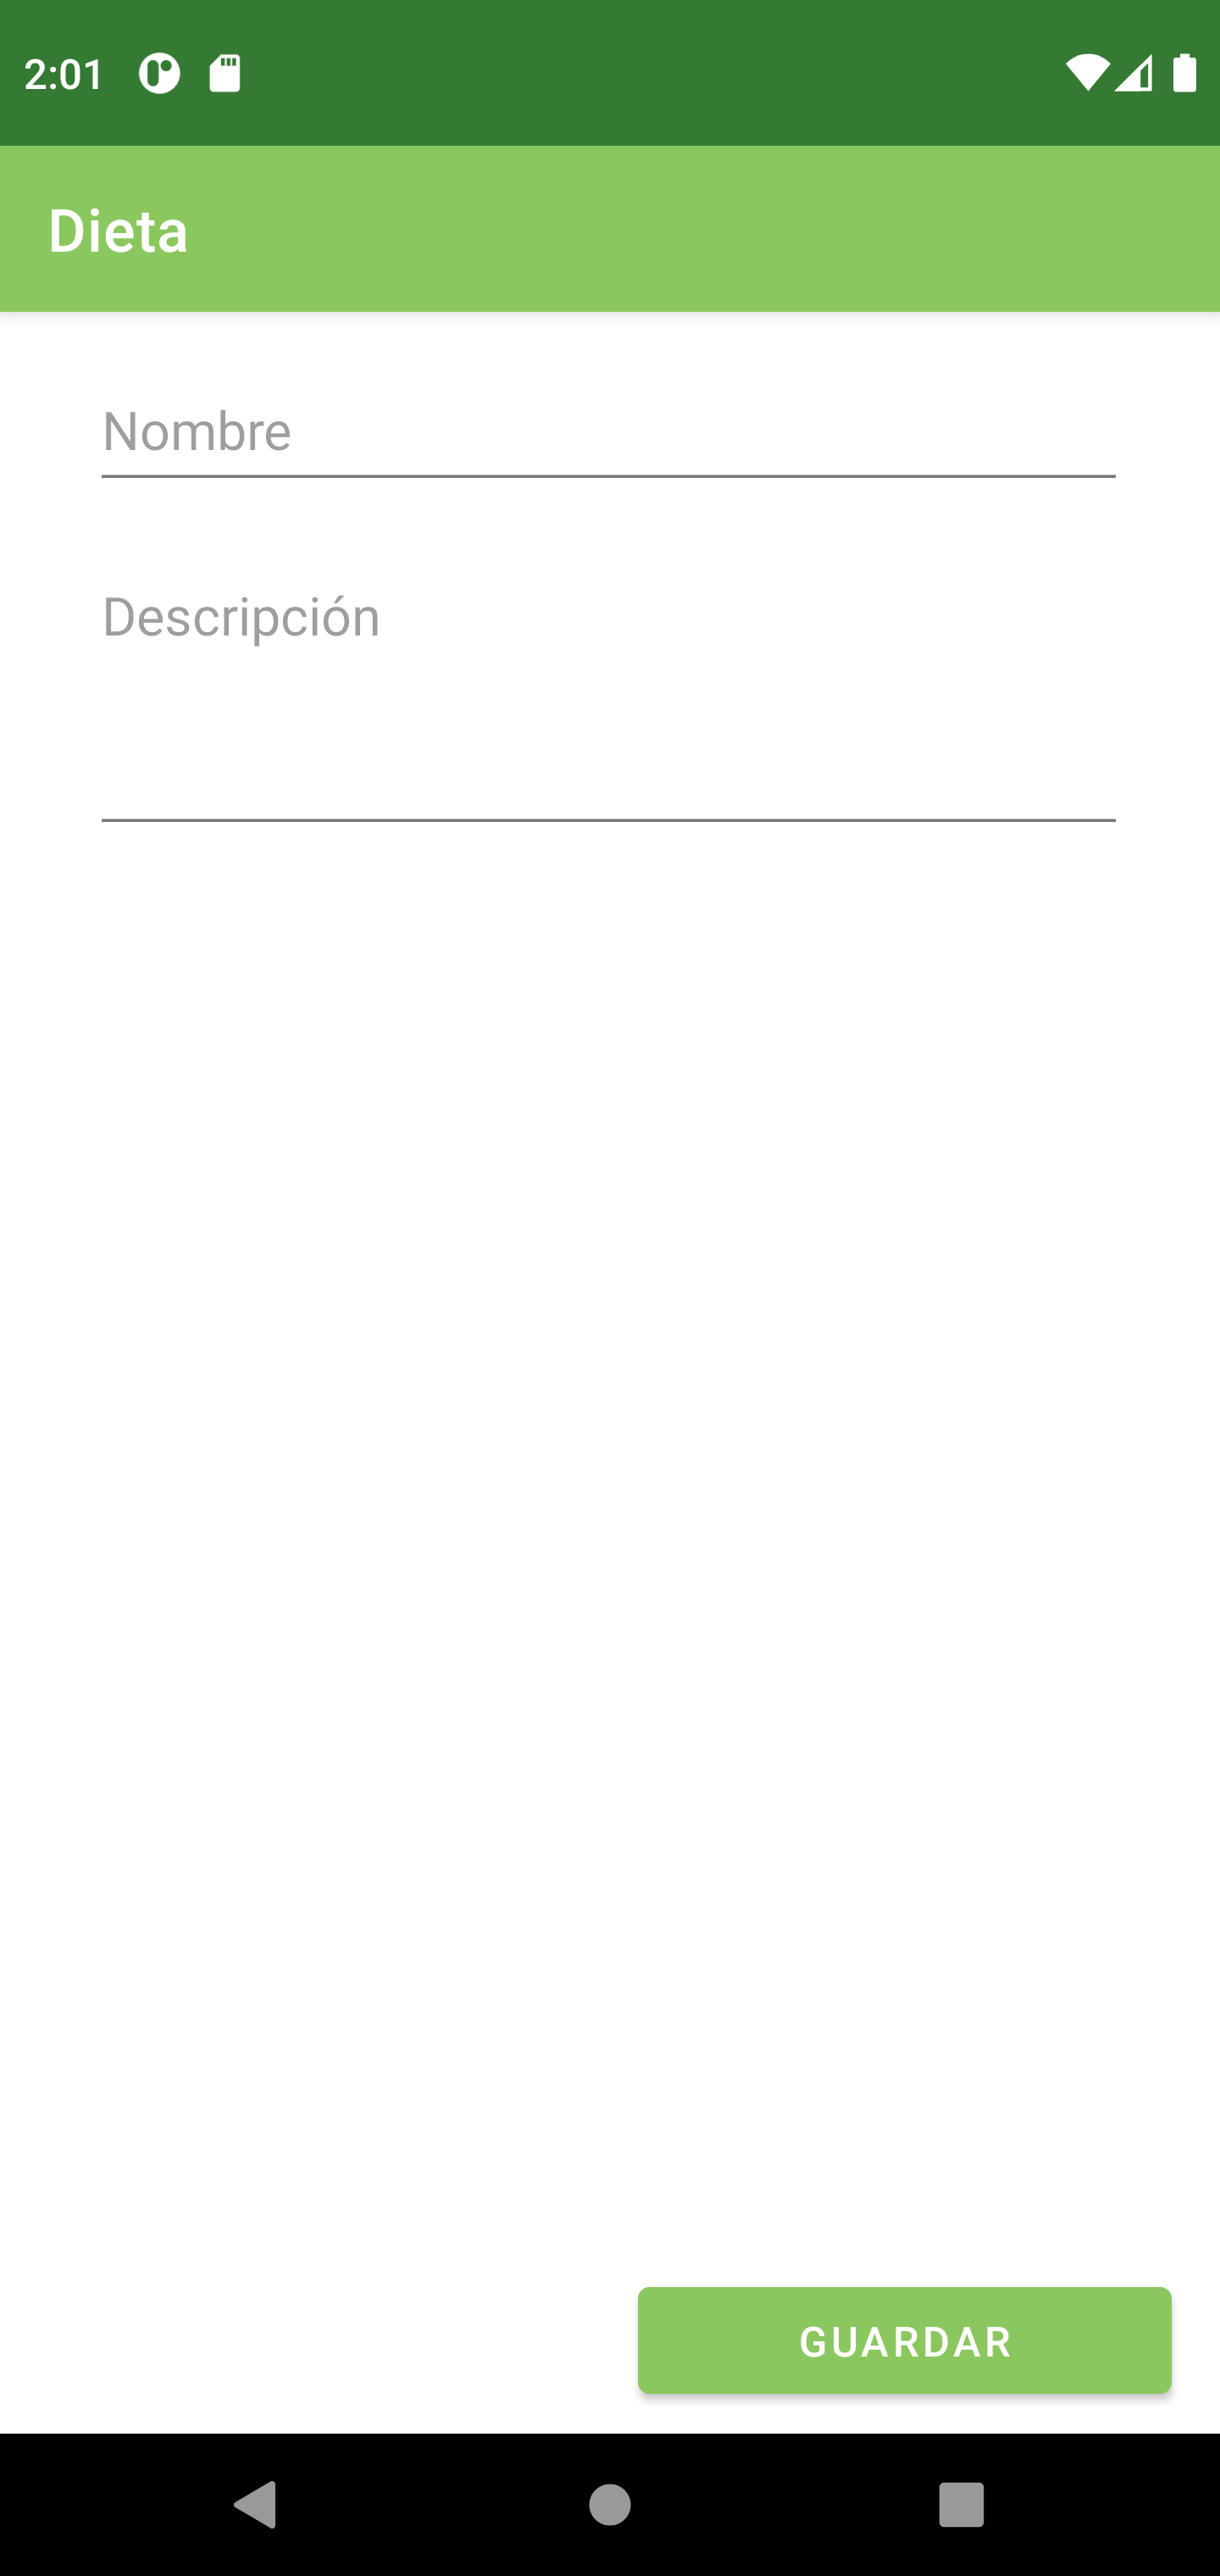
\includegraphics[width=0.4\textwidth]{Images/Annexes/adminCreateDiet2.png}}
    \caption{Crear una dieta}
    \label{fig:crear_dieta}
\end{figure}


\subsection{Todas las dietas del sistema}
Mediante esta opción el administrador puede ver todas las dietas de la aplicación \ref{fig:todas_dietas}, tanto las publicadas como las privadas, al seleccionar la opción se le mostrará un listado con todas las dietas, el número de me gustas y vistos de cada dieta y su estado, es decir si esta publicada o no, también dispondrá de un filtro dinámico en la parte superior de la vista para filtrar las dietas.

El administrador podrá acceder al detalle de cada dieta pulsando ``Ver detalle`` y podrá modificar y/o eliminar la dieta así como cambiar su estado de publicación.

\begin{figure}[H]
    \centering
    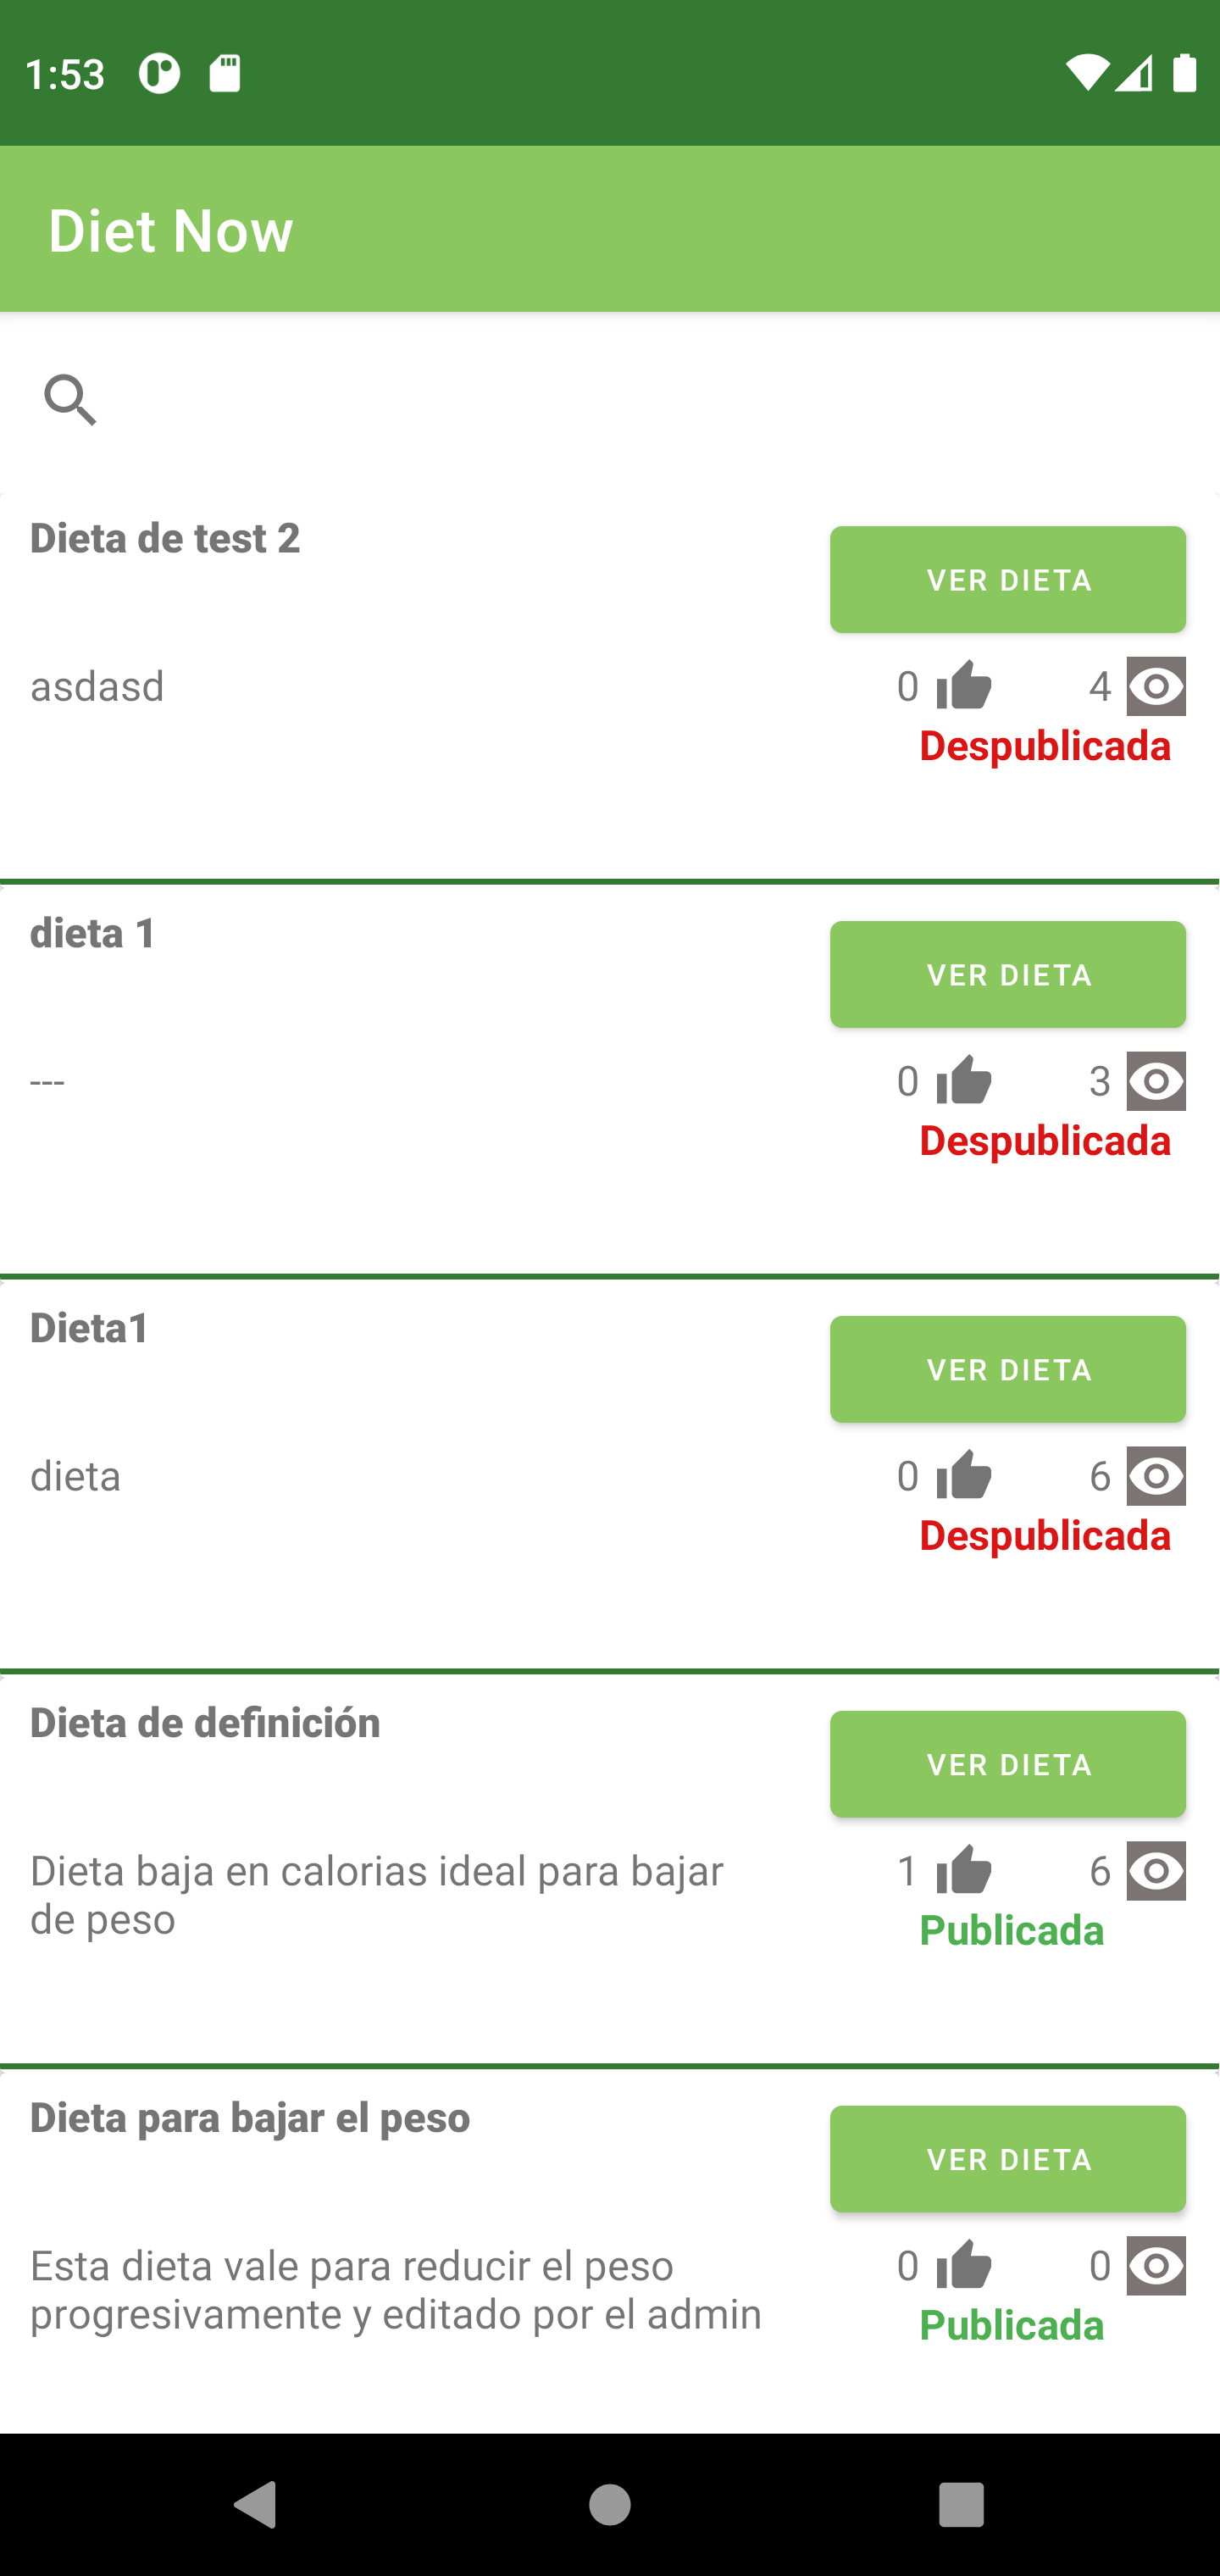
\includegraphics[width=0.4\textwidth]{Images/Annexes/allSysDiets.png}
    \caption{Vista de todas las dietas del sistema}
    \label{fig:todas_dietas}
\end{figure}


\subsection{Mis dietas creadas}
El administrador puede desarrollar está acción de la misma manera que lo haría un deportista, como se aprecia en el apartado \ref{user_my_created_diets}.

\subsection{Ver perfil}
Con esta opción, un administrador accede a su perfil donde se mostrará su información personal y la información del sistema, en esta vista podrá cambiar su imagen de perfil, editar su perfil, cerrar sesión y eliminar cuenta.\ref{fig:admin_profile}

\begin{figure}[H]
    \centering
    \subfigure{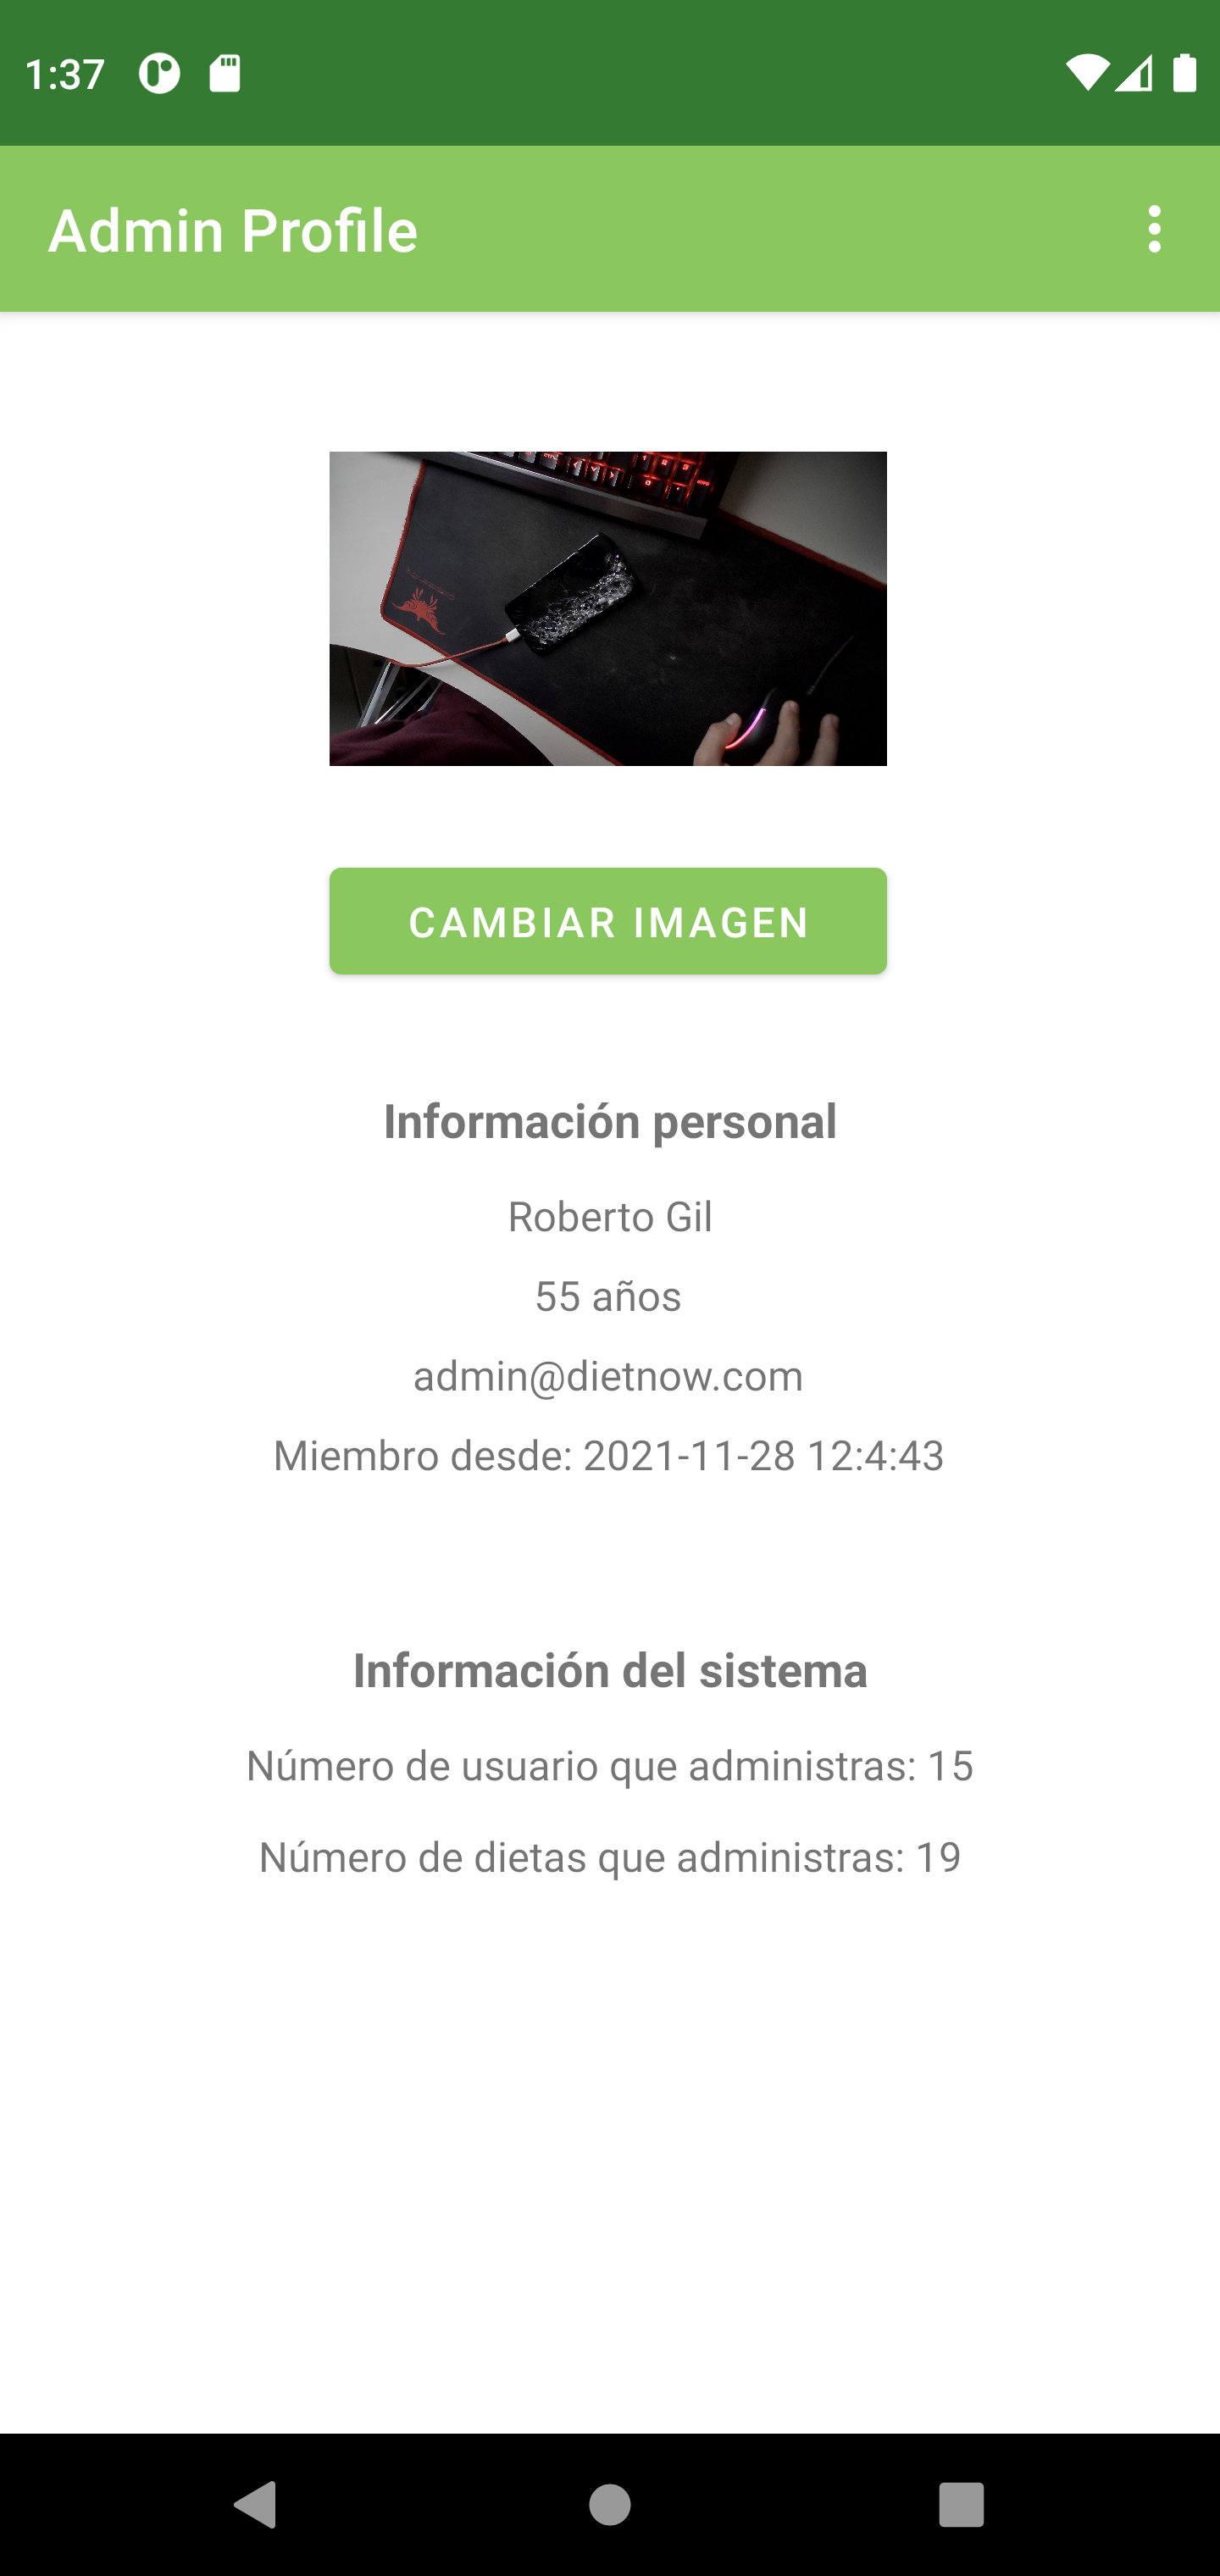
\includegraphics[width=0.4\textwidth]{Images/Annexes/adminProfile.png}}
    \subfigure{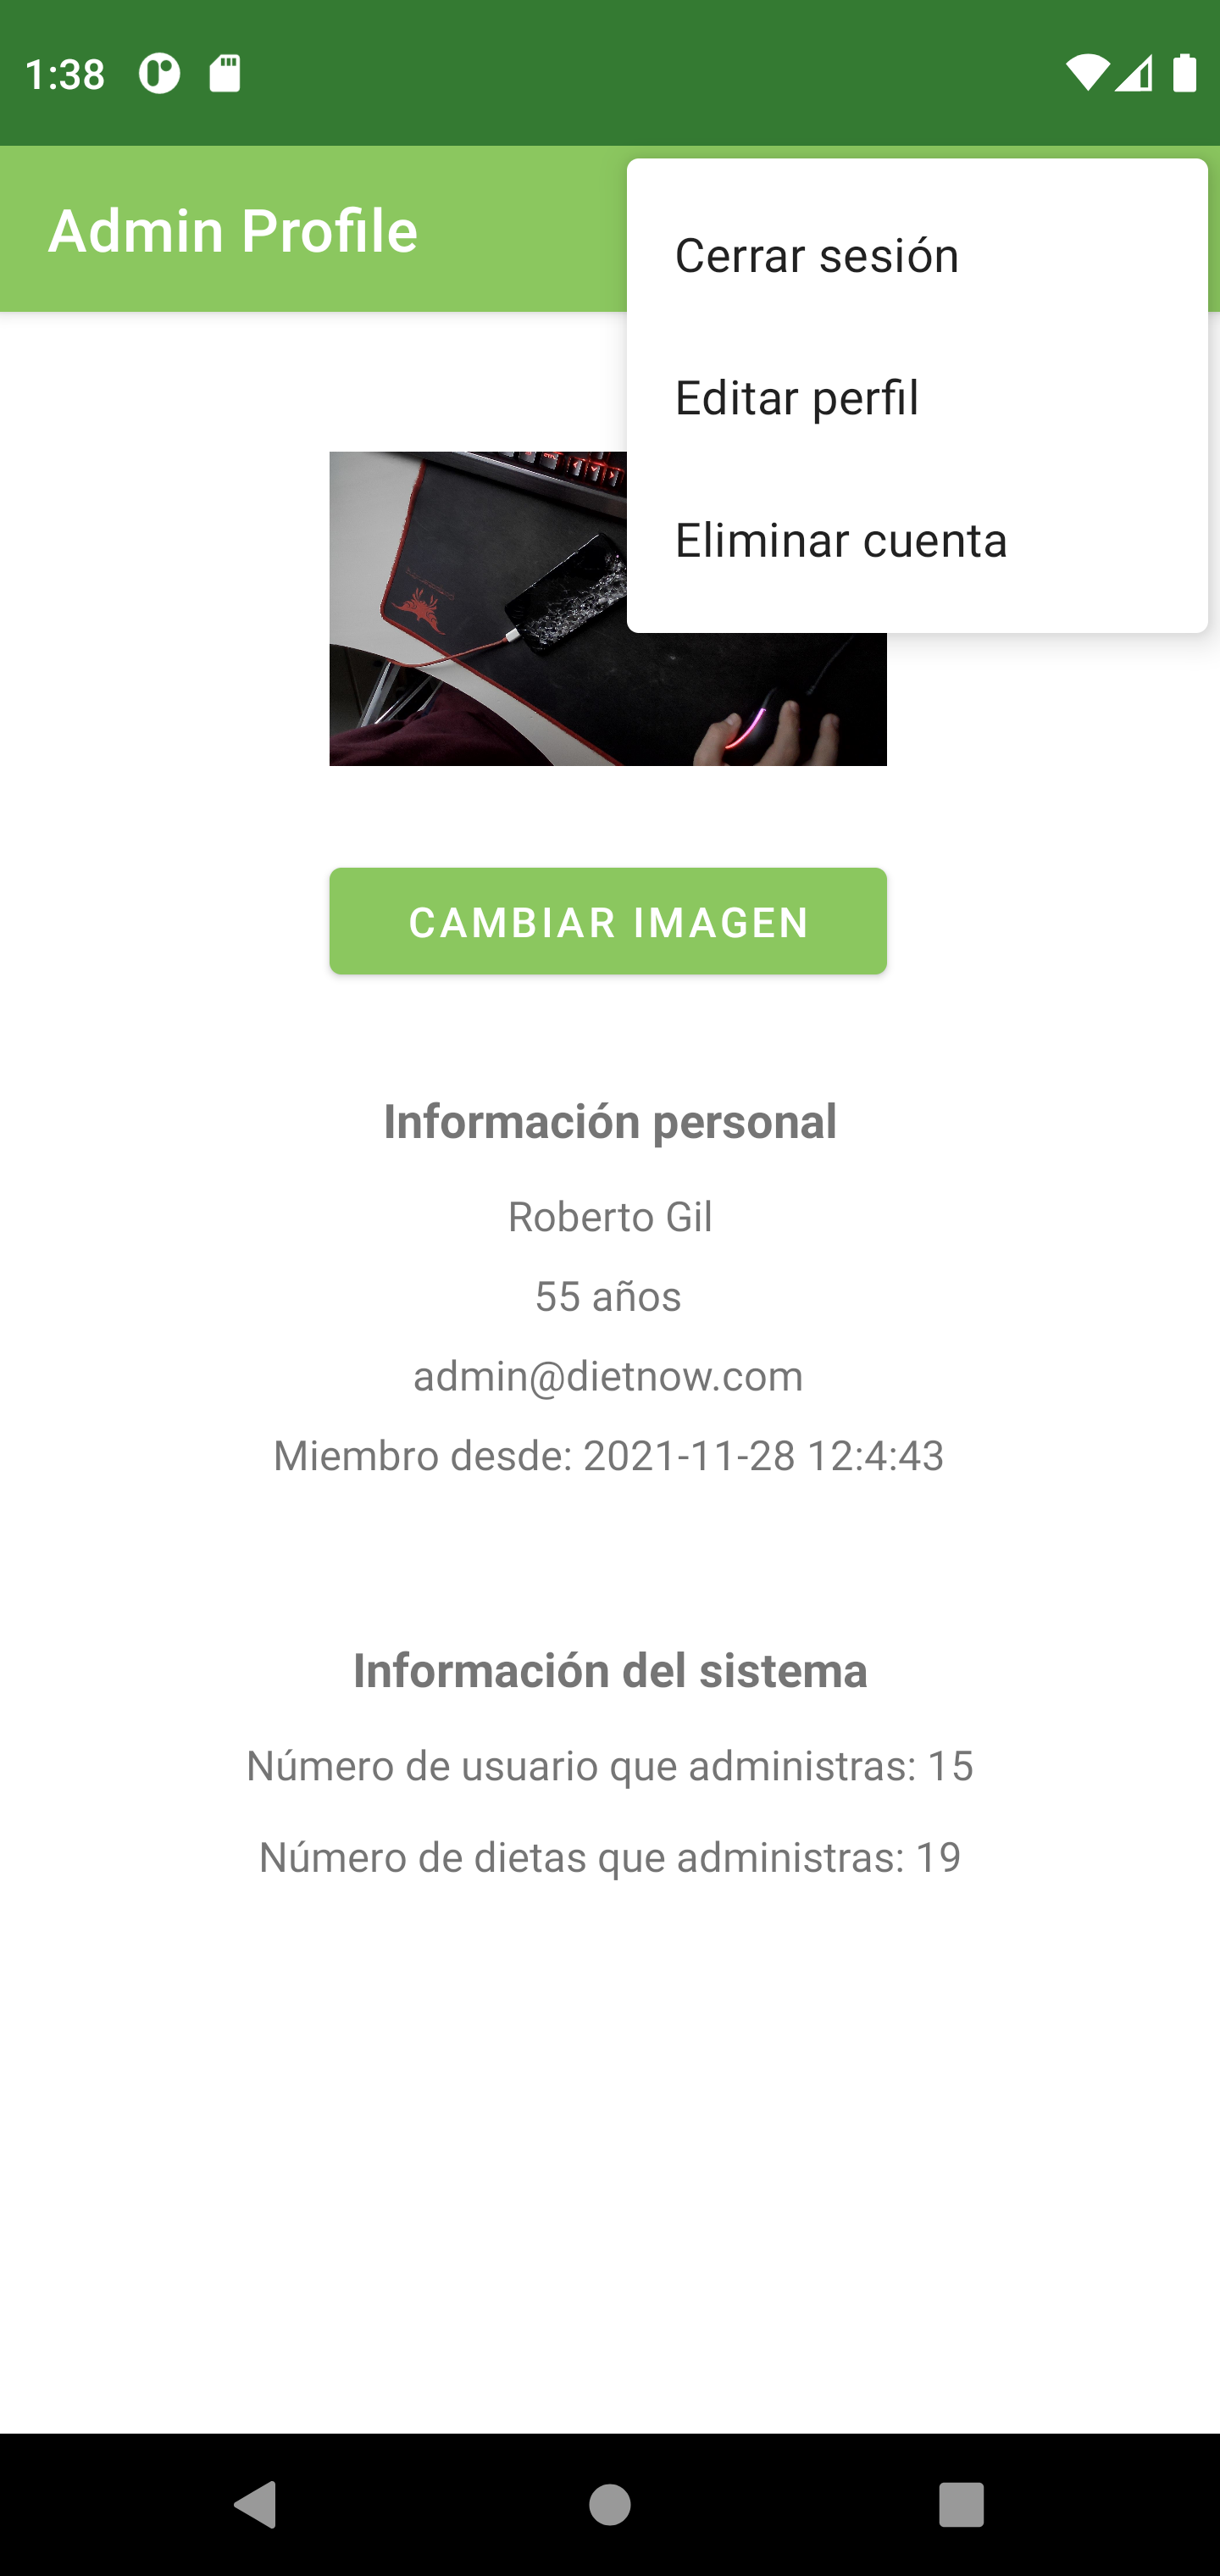
\includegraphics[width=0.4\textwidth]{Images/Annexes/adminProfile2.png}}
    \caption{Vista de ver perfil de un administrador}
    \label{fig:admin_profile}
\end{figure}